\documentclass[12pt,a4paper,notitlepage]{article}
\usepackage[utf8]{inputenc}
\usepackage[english]{babel}
\usepackage[T1]{fontenc}
\usepackage[affil-it]{authblk}
\usepackage[backend=biber,
			style=authoryear-icomp,
			sortlocale=de_DE,
			natbib=true,
			isbn=false,
			doi=false,
			bibstyle=authoryear,
			]{biblatex}
\usepackage{eurosym}
\usepackage{enumitem}
\usepackage{url}
\usepackage{blindtext}
\usepackage{hyperref}
\usepackage{breakurl}
\usepackage{amsmath}
\usepackage{titling}
\usepackage{amsfonts}
\usepackage{amssymb}
\usepackage{pgfplots}
\usepackage{caption}
\usepackage{subcaption}
\usepackage{graphicx}
\usepackage{dcolumn}
\usepackage{tikz-3dplot}
\usepackage{subcaption}
\usepackage{float}
\usepackage{adjustbox}
\usepackage{multirow,rotating}
\usepackage[autostyle]{csquotes}
\usepackage[toc,page]{appendix}
\usepackage{lscape}
\usepackage{sidecap}
\usepackage{todonotes}
\usepackage{booktabs}
\usepackage{multirow}
\usepackage{bm}
\usepackage{eurosym}
\usepackage{pdflscape}
\usepackage{geometry}
\geometry{a4paper,left=30mm,right=20mm, top=2cm, bottom=2cm} 

\addbibresource{Textmining.bib}
\ExecuteBibliographyOptions{maxcitenames=2,mincitenames=1}
\renewcommand*{\mkbibnamelast}[1]{\textsc{#1}}

\title{Matching agendas}
\date{\today}

\author{Franziska Löw
  \thanks{Electronic address: \texttt{loewf@hsu-hh.de}}}
\affil{Department of Industrial Economics,\\ Helmut Schmidt University,\\ Hamburg, Germany}

\begin{document}
\begin{titlepage}
	\maketitle
	\begin{abstract}
	To measure the political slant of german online newspaper the topics addressed in newspapers are compared with topics addressed in press releases of political parties. To find the latent topics in the corpus a structural topic model is conducted. 

	\end{abstract}

\end{titlepage}

\tableofcontents

\pagebreak

%------------------------------------------------%
%----------------- Begin paper -------------------%
%------------------------------------------------%

\section{Introduction}

In recent years, the media and their role in the perception and decision of individuals in the political context have been increasingly subject to criticism. Critics accuse the media of reporting biased on certain parties or political events and thus influencing the political consciousness of voters. This raises the unavoidable question of what biased reporting actually means or, on the contrary, what objective reporting is and if this is even possible. A journalist who writes an article about a certain topic puts rough facts (e.g. figures on economic indicators) into a context, such that each article is shaped by the subjectivity of this journalist. Similarly, an editor of a media outlet has to select the topics to be discussed in the medium from a large pool of reports. Thus, to a certain extent, media is always filtered by journalists' perceptions and editorial decisions. 

A legitimate question, however, could be which factors or incentives lead to the selection or deselection of certain topics. On the one hand, one could assume that editors select the topics and articles that correspond to their own political views. A profit-maximizing editor, on the other hand, would tend to adapt the selection to readers' preferences. However, in the case of public services, one would assume that the reporting reflects the mandate to contribute to the formation of individual and public opinion and to act politically and economically independently.

In order to answer these and other media-related questions in the political context, quantifying the content of media is a prerequisite. One of the key challenges is to determine the features that are used to describe media content (audio, video, text). Studies that rely on quantifying media content for their analyses use, for example, visibility (how often political actors appear in the media) or tonality (how they are evaluated). Other studies examine the topics discussed or the language used in the media, in order to identify whether political actors are able to place their own policy positions in the media. Leading studies from economic literature, for example, examine how often a newspaper quotes the same think tanks \citep{groseclose_measure_2005, lott_is_2014} or uses the same language \citep{gentzkow_media_2004} as members of Congress. 

Following this approach, the present paper compares topics discussed in media outlets with topics addressed in the press releases of the parties in the german "Bundestag", to measure the ideological content of several online news services in Germany. The dataset contains over 15.000 online news articles from seven major news provider as well as 2.666 press releases of the parties in the german "Bundestag", both dated from June 1, 2017 to March 1, 2018. As the German federal elections took place on 24th of September 2017 and the formation of the government has taken up a period of about five months, the articles considered inform their readers about both the election promises of the parties (before the election) and the coalition talks (after the election). To discover the latent topics in the corpus of text data, the structural topic model (STM) developed by \citet{roberts_model_2016} is applied. The STM is an unsupervised machine learning approach that models topics as multinomial distributions of words and documents (as a synonym for news articles) as multinomial distributions of topics, allowing the incorporation of external variables that affect both, topical content and topical prevalence. The results of the generative process of the STM are two posterior distributions: One for the topic prevalence in a document (what is the article or press release about?) and one for the content of a topic (what is the topic about?). The topic prevalence is used to estimate a slant-index by estimating the correlation between the posterior distribution of topics in press releases with the posterior distributions of topics in news articles. The resulting slant index of a newspaper is used to identify possible drivers of the differences between the media outlets: 1) the political orientation of consumers/consumer preferences, 2) current poll values, 3) differences between public or private media. 1) and 2) no evidence for causality! 

The research contribution of this paper is twofold: First, a new method for the calculation of the slant-index is presented that allows an extensive content analyses of newspaper coverage and party press releases and at the same time reduces human induced bias and makes research more traceable and comparable. In addition, a new dataset of online news is used, which has a significant relation to the current discussion of the media in the political context. 

The remaining course of the paper is as follows: The following section provides an overview of the related literature. Section \ref{ch_elections} gives an introduction to the political trends within the considered time (June 2017 to March 2018). The data used to conduct the model is described in section \ref{ch_data}. Section \ref{ch_generativeProcess} explains the generative process of the structural topic model as well as the selected parameters to run the model. The empirical analysis is conducted in section \ref{ch_regression}. 

%-------------------------------------------------------%
%----------------- Literature Review -------------------%
%-------------------------------------------------------%

\section{Literature}

This paper combines research in the field of media bias with the literature of computer-aided analysis of text data in general and topic models in particular. To put this paper into context within both research areas, this section starts with an overview of the literature on media bias, mainly limited to the economic literature and referring to related disciplines where appropriate. Subsequently, a literature overview on topic models in the relevant research areas is given. 

The concept of media bias has been investigated in different research fields in the social sciences (e.g. politics, communication research, economics), although based on different hypotheses and assumptions. The majority of this research attempts to answer one or more of the following questions: (1) Is media biased? (2) how and why does it emerge? (3) What influence does it have on (political/societal) outcomes? From an economic point of view, question (2) analyses the market dynamics that lead to a possible bias.  

The general hypothesis within economic literature is that (1) different media outlets tend to report "biased" or "slanted" \citep{groseclose_measure_2005, lott_is_2014} and that (2) media reporting about political news may have a profound influence on political outcomes \citep{gentzkow_media_2004, stromberg_radios_2004, dellavigna_fox_2006, snyder_press_2010, gentzkow_television_2006}. Basically, media bias can be influenced by the supply side and reflect the preferences of journalists \citep{baron_persistent_2006}, editors or owners \citep{besley_handcuffs_2006}. Alternatively, media distortion can also reflect the profit-maximising behaviour of news providers who are responsive to consumer preferences. In this case, the distortion would rather be initiated by the demand side \citep{mullainathan_market_2005, gentzkow_media_2006, suen_self-perpetuation_2004}. 

% 2 sided markets
Since private media outlets are almost exclusively platforms, that connect the market of advertising with the reader market, broadcasters coordinate the two sides to exploit the indirect network effects between them. Advertising-financed media generate their sales on the market side of the advertisers, who in turn are attracted by the readers as potential customers. \citet{anderson_media_2006} argue, that competition for viewers of the demographics most desired by advertisers implies that programming choices will be biased towards the tastes of those with such demographics. However, \citet{gentzkow_what_2010} find that media outlets respond strongly to consumer preferences for like-minded news, which account for 20 percent of the variation in measured slant in their sample of U.S. daily newspapers.

% ---- Is media biased? ---- %
In order to answer the question whether the media is biased, the preliminary question of what media bias means has to be answered. In order to arrive at a better operational definition of bias, some scholars argue that an objective news report is a neutral or balanced report, thus one where all sides are equally represented according to some kind of benchmark for balance or neutrality \citep{eberl_one_2017}. 

% ---- What is media bias? How to measure political content? ---- %

%-- umschreiben! (zu doll von Hansen geklaut)
The major empirical challenge for the analysis of media content, and one I address head on in this paper, is to convert the raw text into meaningful quantities which can be systematically analysed. 
%--

Some approaches focus on the quantitative visibility from a political entity, e.g. how often this entity is mentioned in the article. The frequency of mentioning or mere visibility is then used as an indicator of a party's media coverage \citep{oegema_personalization_2009, eberl_one_2017, junque_de_fortuny_evaluating_2014}. Although this approach analyses the visibility of political actors, it says nothing about the way in which they are covered. The concept of valence framing suggests that public awareness of parties is affected depending on whether they are highlighted with positive or negative aspects in the media \citep{de_vreese_valenced_2006, hurtikova_importance_2017}. To take into account this effect, sentiment analysis is a commonly used approach to measure how parties are discussed in media. To measure tonality in a text, studies differ between manually coded data \citep{eberl_one_2017, dewenter_can_2018} and dictionary-based analysis \citep{junque_de_fortuny_media_2012}. To conduct the latter, a lists of words (dictionary) associated with a given emotion, such as negativity is pre-defined by the analyst. The document is then deconstructed into individual words and the frequencies of words contained in a given dictionary are calculated. \citet{junque_de_fortuny_media_2012} count the sentiment words in a window of two sentences before and after the mention of a political party and assuming uniformity of sentiment distribution among parties to measure the bias.\footnote{A similar approach for target identification with a 10-word window is used in \citet{balahur_sentiment_2013}} 

A further approach to quantifying media content in terms of political content is the evaluation of domain-specific language. \citet{groseclose_measure_2005} count the times that particular media outlet cites various think tanks and policy groups, and then compare this with the times that members of Congress cite the same groups. Similarly \citet{gentzkow_what_2010} define a set of all phrases used by members of Congress in the 2005 Congressional Record, and identify those that are used much more frequently by one party than another. In both cases, news articles are scanned for the previously defined language. News providers who quote think tanks more frequently or use sentences used by one party rather than another have a bias toward that party. 

In addition to domain-specific language, topics can also be used as an indicator of political content, following the assumption that parties want the media agenda to be congruent with their own agenda to define the issue-based criteria on which they will be evaluated by voters. \citet{eberl_one_2017} compares topics in press releases of political parties with topics in news agencies in order to find out which media cover the topics addressed by the parties. 

%-- umschreiben! (zu doll von Hansen geklaut)
 The main methodological contribution in this paper is to use computational linguistics, and particularly the combination of topic modelling and dictionary methods, in order to examine the content of what central banks are trying to communicate to the markets and the public.

The first obvious advantage of the use of automated techniques rather than a purely narrative approach to study the statements is scalability without concerns about consistency of the application of the method. With automated methods it is then easy to extend the sample to include more recent data, other sources of communication such as FOMC speeches, or to extend it to other central banks.

In terms of the computational approaches, I use a structural topic model (STM) and dictionary methods to extract the content of online news articles of seven major news provider and press releases of the parties in the German Bundestag. 
%--

% -----  STM --------
The STM developed by \citet{roberts_model_2016} is a recent extension of the standard topic modelling technique, labeled as latent Dirichlet allocation (LDA), which refers to the Bayesian model in \citet{blei_latent_2003} that treats each word in a topic and each topic in a document as generated from a Dirichlet - distributed prior.\footnote{See also \citet{griffiths_probabilistic_2002}, \citet{griffiths_finding_2004} and \citet{hofmann_probabilistic_1999}. \citet{pritchard_inference_2000} introduced the same model in genetics for factorizing gene expression as a function of latent populations.} Since its introduction into text analysis, LDA has become hugely popular and especially useful in political science.\footnote{see \citet{blei_probabilistic_2012}, \citet{grimmer_text_2013} and \citet{wiedmann_text_2016} for an overview in social science and \citet{gentzkow_text_2017} give an overview of text mining applications in economics.} \citet{wiedmann_text_2016} uses topic model methods on large amounts of news articles from two german newspapers published between 1959 and 2011, to reveal how democratic demarcation was performed in Germany over the past six decades. \citet{paul_cross-collection_2009} compares editorial differences between media sources, using cross-collection latent Dirichlet allocation (ccLDA), an LDA-based approach that incorporates differences in document metadata. They use a dataset of 623 news articles from August 2008 from two American media outlets - msnbc.com and foxnews.com - to compare how they discuss topics. Reviewing the top words of the word-topic distribution, they find some content differences between the two media sources under review.

Furthermore, the model has been applied to multiple academic fields: \citet{roberts_structural_2014} uses STM to analyze open-ended responses from surveys and experiments, \citet{farrell_corporate_2016} applies the model to scientific texts on climate change, revealing links between corporate funding and the framing of scientific studies. \citet{mishler_using_2015} show that "STM can be used to detect significant events such as the downing of Malaysia Air Flight 17" when applied to twitter data. Another study shows how STM can be used to explore the main international development topics of countries'€™ annual statements in the UN General Debate and examine the country-specific drivers of international development rhetoric \citep{baturo_what_2017}. \citet{mueller_reading_2016} use newspaper text to predict armed conflicts in different regions. They use the estimated topic shares in linear fixed effects regression to forecast conflict out-of-sample. \citet{roberts_navigating_2016} use STM to examine the role of partisanship in topical coverage using a corpus of 13,246 posts that were written for 6 political blogs during the course of the 2008 U.S. presidential election. With the aim of revealing the effect of partisan membership on topic prevalence, each blog is assigned to be either liberal or conservative. To explore the differences between the two, they look at the expected proportion of topics and examine the posts most associated with a respective topic. This approach is similar to \citet{roberts_model_2016}. 

The main contribution of this paper relative to the above mentioned research work is that I combine the effect of topic correlation \citep{eberl_one_2017} and sentiment analysis \citep{dewenter_can_2018, junque_de_fortuny_evaluating_2014, eberl_one_2017} to estimate the slant index of media. I also apply different tools from computational linguistics (both STM for topic modelling and dictionary methods to measure sentiment).

The remainder of the paper proceeds as follows... 

% -------------------------
% Background Bundestagswahl
% -------------------------
\section{Background information}\label{ch_elections}

\subsection{The political situation in Germany (June 2017 - March 2018)}

The articles analyzed in this paper cover a period from June 1, 2017 to March 1, 2018 and thus cover both the most important election campaign topics for the Bundestag elections on September 24, 2017 and the process of forming a government that lasted until February 2018. After four years in a grand coalition with the Social Democrats (SPD), German Chancellor Angela Merkel, member of the conservative party CDU/CSU (also known as Union), ran for re-election. The SPD nominated Martin Schulz as their candidate. 

On the right side of the political spectrum, AfD (alternative for Germany) managed to be elected to the German Bundestag for the first time in 2017. The political debate about the high refugee numbers of the past years brought a political upswing to the AfD, which used the dissatisfaction of parts of the population to raise its own profile. In the course of the reporting on the federal elections, leading party members of the AfD as well as party supporters repeatedly accused the mass media of reporting unilaterally and intentionally presenting the AfD badly.

After the election, the formation of a government was difficult due to the large number of parties elected to the Bundestag and the considerable loss of votes by the major parties CDU/CSU and SPD. Since all parties rejected a coalition with the AfD, numerically only two coalitions with an absolute parliamentary majority were possible: a grand coalition ("GroKo" - from the German word Groߟe Koalition) of CDU/CSU and SPD, and a Jamaica coalition (coalition of CDU/CSU, FDP (economic liberal party) and B90/Die Grünen (Bündnis 90/Die Grünen, green party)). The grand coalition was initially rejected by the SPD. The four-week exploratory talks on the possible formation of a Jamaica coalition officially failed on November 19, 2017 after the FDP announced its withdrawal from the negotiations. FDP party leader Christian Lindner said that there had been no trust between the parties during the negotiations. The main points of contention were climate and refugee policy. CDU and CSU regretted this result, while B90/Die Grünen sharply criticized the liberals'€™ withdrawal. The then Green leader Cem Özdemir accused the FDP of lacking the will to reach an agreement.

After the failure of the Jamaica coalition talks, a possible re-election or a minority government as alternatives were discussed in the media before the SPD decided to hold coalition talks with the CDU/CSU. This led to great resistance from the party base, which called for a party-internal referendum on a grand coalition. After the party members voted in favor of the grand coalition, a government was formed 171 days after the federal elections. 

Figure \ref{fig_polls} shows that support for the two major popular parties has been declining in recent months since August 2017, with the CDU/CSU again showing positive survey results since November 2017.\footnote{For each party the survey results of the seven major institutes are considered. To calculate a smooth line for each party on each day, the moving average within 15 days (7 before the day, 7 after the day, and the day itself) is estimated. The data source is https://www.wahlrecht.de/.} However, the poll results of the SPD have been falling since March 2017. At the same time, the AfD in particular has been recording increasingly positive survey results since June 2017.  

\begin{figure}[H]
\begin{center}
	\caption{Election Polls}
	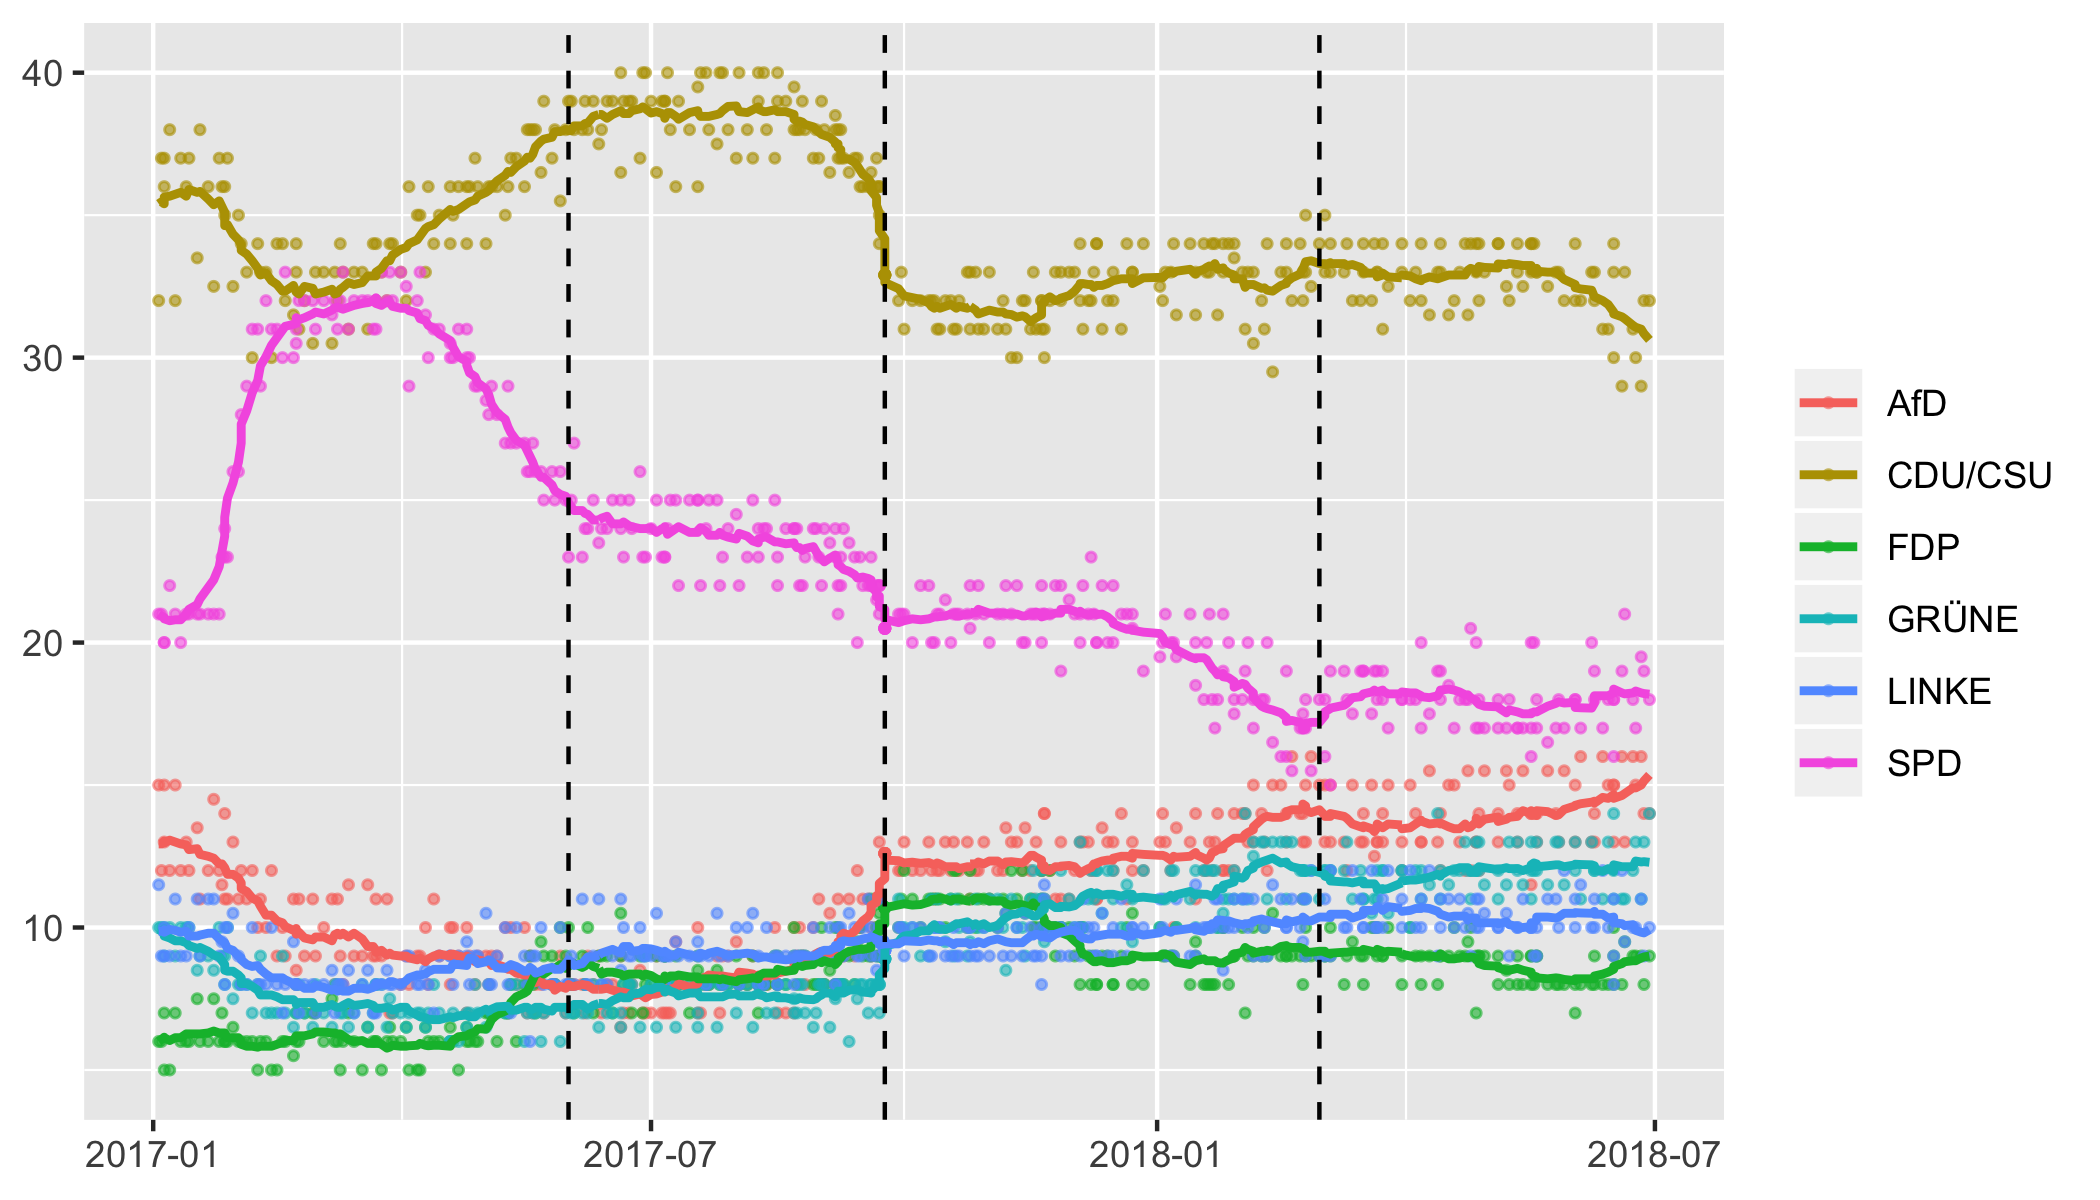
\includegraphics[width=0.9\textwidth]{../figs/polldata}
	\label{fig_polls}
	\end{center}
\end{figure}

\subsection{German online news market}

The analysis performed in this paper is based on the news articles of the following news websites: Bild.de, DIE WELT, FOCUS ONLINE, SPIEGEL ONLINE, stern.de, ZEIT ONLINE, Tagesschau.de. As can be seen from  Figure \ref{fig_visits}, these media outlets are among the top 30 German online news providers in the period under review in terms of visits.\footnote{The term visit is used to describe the call to a website by a visitor. The visit begins as soon as a user generates a page impression (PI) within an offer and each additional PI, which the user generates within the offer, belongs to this visit.}. Of the selected websites only Tagesschau.de belongs to the public broadcasting and is financed thus by coercive fees - the remaining websites belong to privately managed media houses. The main source of income for private media is digital advertising, even though paid content is playing an increasingly important role. However, according to a survey on digital news by the Reuters Institute \citep{newman_reuters_2018} only 8\% of respondents pay for online news. The online survey for German data was undertaken between 19th - 22nd January 2018 by the Hans Bredow Institute\footnote{https://www.hans-bredow-institut.de/de/projekte/reuters-institute-digital-news-survey} with a total sample size of 2038 adults (aged 18+) who access news once a month or more. Among other questions, participants were asked which news sources they use to access news online.\footnote{The exact question was: "Which of the following brands have you used to access news online in the last week (via websites, apps, social media, and other forms of Internet access)? Please select all that apply"} The results displayed in Figure \ref{fig_reuters1} indicate that the media used for the analysis play a relevant role in their consumption.

\begin{figure}[H]
	\begin{center}
	\caption{Selected news brands}
		\begin{subfigure}[normla]{0.49\textwidth}
			\caption{Total visits in million (Jan 2018)}
			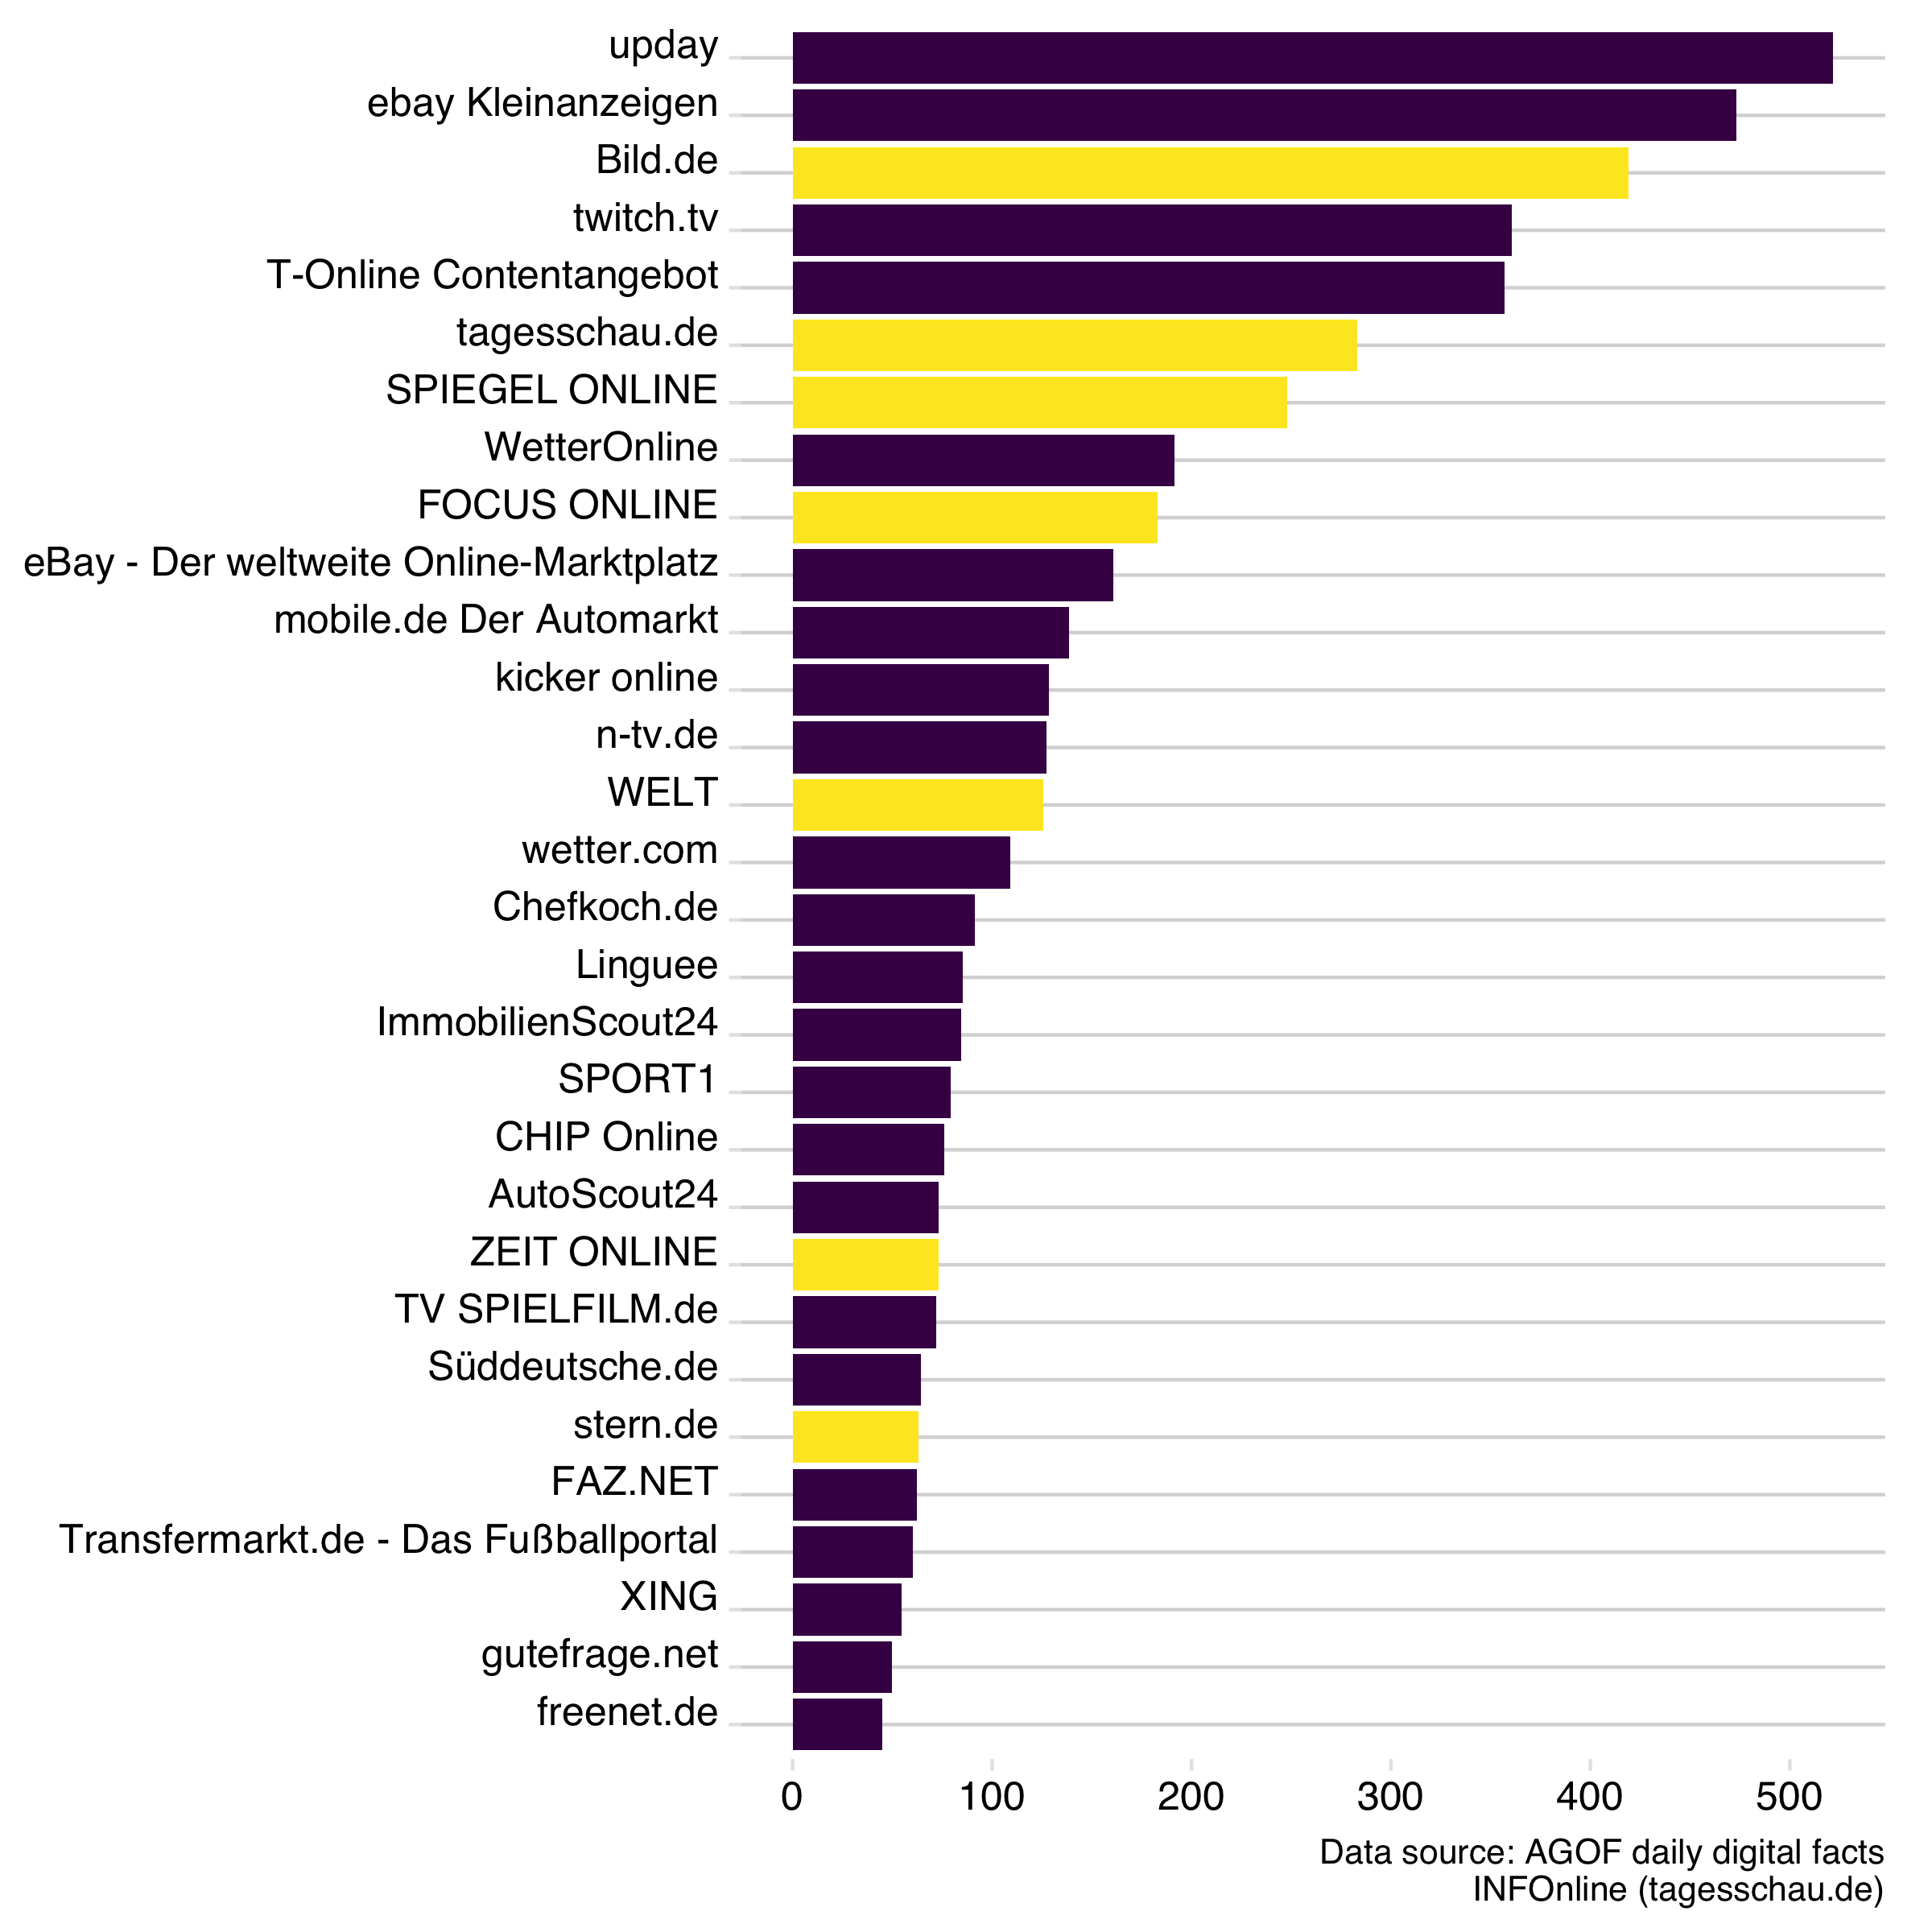
\includegraphics[width=\textwidth]{../figs/visits}
			\label{fig_visits}
		\end{subfigure}
		\begin{subfigure}[normla]{0.49\textwidth}
			\caption{Use of a brand to access news online}
			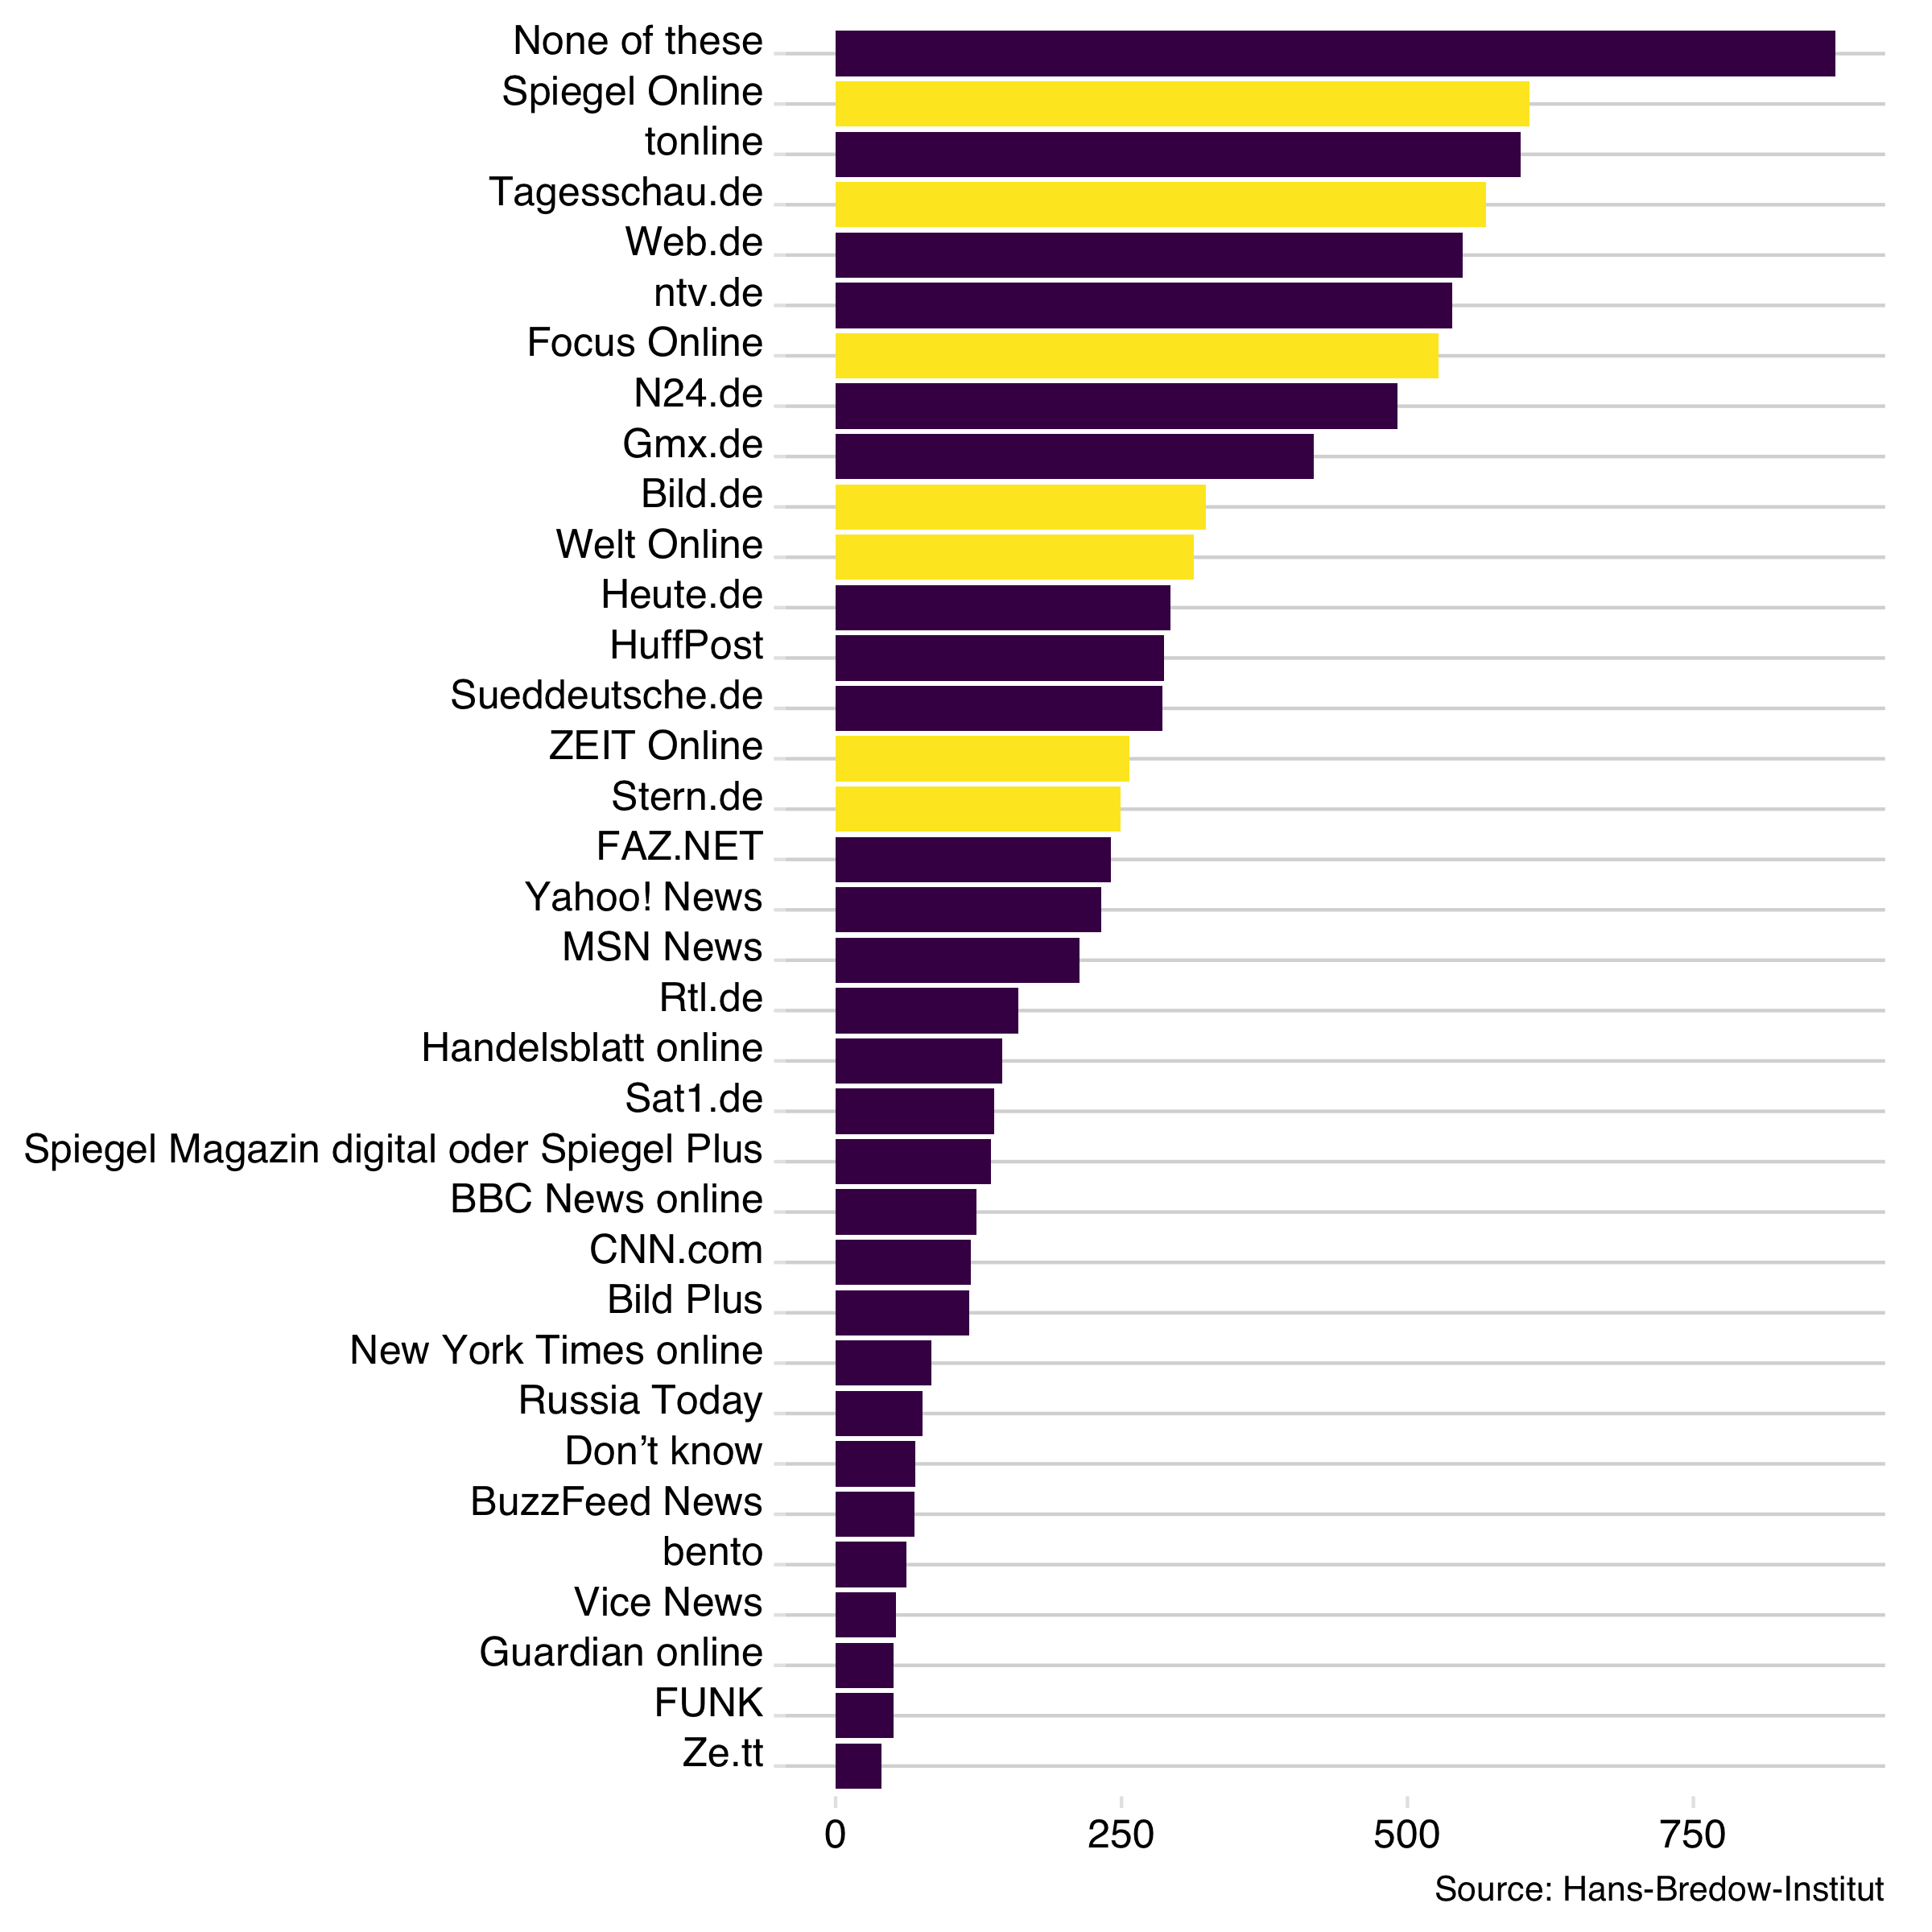
\includegraphics[width=\textwidth]{../figs/reuters1}
			\label{fig_reuters1}
		\end{subfigure}
	\end{center}
\end{figure}

In addition to media consumption, the participants of the survey on digital news were asked where they would rank themselves on a political scale defined by "left", "center" and "right".\footnote{The exact question was: Some people talk about 'left', 'right' and 'centre' to describe parties and politicians. (Generally socialist parties would be considered ‘left wing’ whilst conservative parties would be considered ‘right wing’). With this in mind, where would you place yourself on the following scale?} Figure \ref{fig_reuters2} shows that a large proportion of the respondents place themselves in the political centre (30\%) or slightly to the right (18.7\%) or the left (22.5\%) of the center. Only a small part would consider themselves to be fairly or very right (6.1\%) or left (8.3\%) of the political spectrum.

\begin{figure}[H]
\begin{center}
	\caption{Political orientation }
	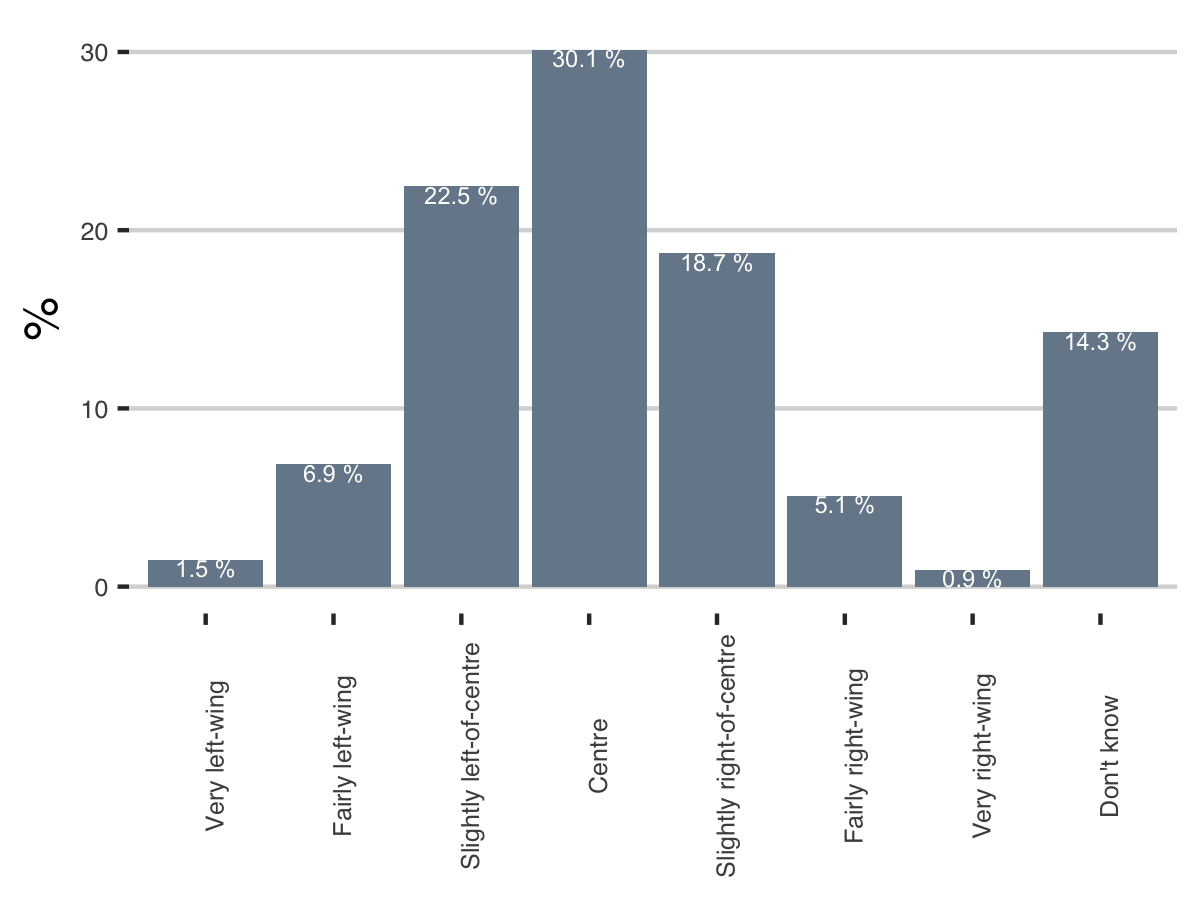
\includegraphics[width=0.5\textwidth]{../figs/reuters2}
	\label{fig_reuters2}
	\end{center}
\end{figure}

Combining both the political orientation and the brand preferences can give an indication about the political orientation of the consumers of a specific medium. Thus, for example, it is possible to answer the question of how many percent of the respondents, who stated that they consume stern.de, classify themselves as rather left of the political spectrum. To calculate this value, the absolute values for each medium-political orientation combination in Figure \ref{fig_reuters3} was divided by the total number of respondents, who consume a specific medium. As the results show, the majority of consumers of ZEIT Online and Spiegel Online place themselves rather on the left, while the opposite is true for Focus Online, Welt Online and Bild.de. Consumers of Tagesschau.de and stern.de would rather place themselves in the center of the political spectrum. 

\begin{figure}[H]
\begin{center}
	\caption{Political orientation }
	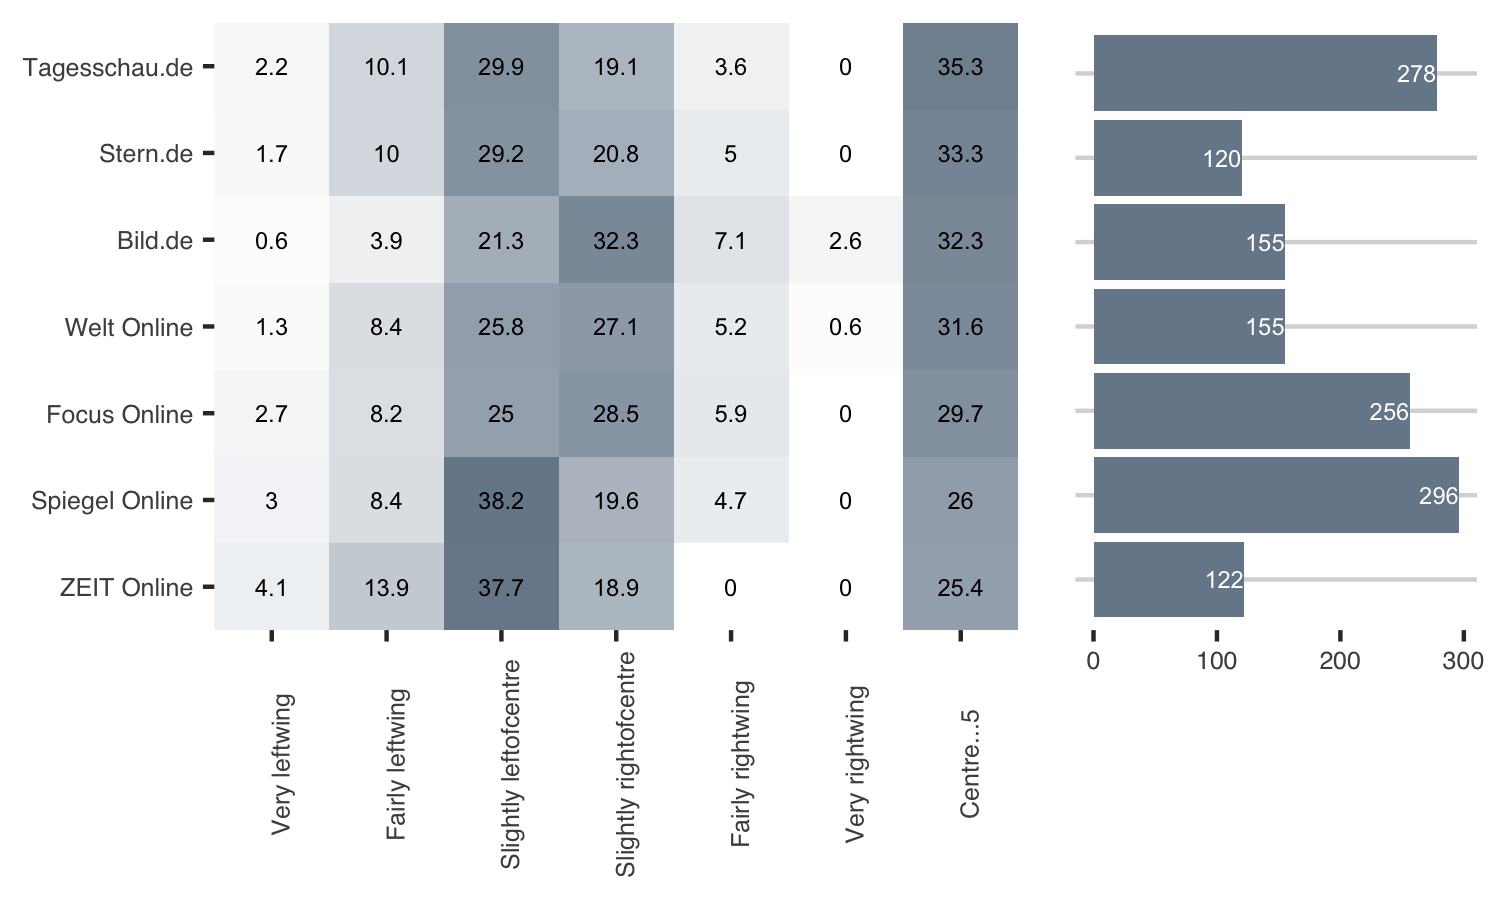
\includegraphics[width=.9\textwidth]{../figs/reuters3}
	\label{fig_reuters3}
	\end{center}
\end{figure}

Based on the finding from \citet{gentzkow_what_2010} that readers prefer like-minded news and that firms respond strongly to consumer preferences, the hypothesis can be made that media reporting of ZEIT Online and Spiegel Online tends to be left biased, while Focus Online and Welt Online are expected to be more biased to the right. However, \citet{anderson_media_2006} argue, that competition for viewers of the demographics most desired by advertisers implies that programming choices will be biased towards the tastes of those with such demographics. This effect would tend to lead news providers to report similarly as they compete for the same customers on the advertising market.

In contrast to the other providers, tagesschau.de is financed by compulsory fees and has the constitutional mandate to contribute to the formation of individual and public opinion and to secure basic provision. This implies a nationwide reception of broadcasting for the general public as well as the supply of a diversified content.\footnote{The mandate of public service broadcasting is based on Art. 5 Para. 1 Sentence 2 of the German Basic Law (Grundgesetz).} This leads to the assumption that the reporting of tagessschau.de is not aligned to the market conditions of the advertising and reader market, but rather reports balanced on all parties and possible topics.


% -----
% Data
% -----
\section{Data}\label{ch_method}

To measure the slant index of a media outlet, the topics discussed in that media outlet are compared to topics discussed in the press releases of political parties. 

Parties want the media agenda to be congruent with their own agenda to define the issue-based criteria on which they will be evaluated by voters \citep{eberl_one_2017, brandenburg_political_2005}. Thus, I assume that parties instrumentalize their press releases in order to highlight issues that they are perceived to be competent on, that they "own" and that are important to their voters \citep{kepplinger_einfluss_2004}. Editors can select from this universe and decide which topics will be discussed in the news. In that sense the ideological content of a newspaper refers to the extent to which the topics promoted by the parties correlate with the topics discussed in the news articles. 

% Ich nehme außerdem an, dass Parteien Themen mit unterschiedlichen "Sentiment" Werten besprechen. Ich vergleiche dieses Sentiment mit dem wert der Zeitungen. 

The following section describes the data on news articles and press releases and how they have processed in order to use them as input for the model.

\subsection{Press releases}\label{ch_press}

The press releases were scraped from the publicly accessible press portals of the parties\footnote{afd.de, spd.de, die-linke.de, fdp.de, gruene.de, cdu.de} and parliamentary groups\footnote{afdbundestag.de, spdfraktion.de, die-linke.de/start/presse/aus-dem-bundestag, fdpbt.de, gruene-bundestag.de/, presseportal.de/nr/7846}. 

It should be noted that there is a legal distinction between press releases from political parties and parliamentary groups in the Bundestag, as parties are financed by membership dues, donations and campaign expenses, while parliamentary groups are financed by state funds. According to Parteigesetzt §25 (2) state funded parliamentary groups may not support parties, as there would be a disadvantaged for parties that are not in the Bundestag. However, since it is difficult to draw the line between the activity of parliamentary groups and election campaign assistance \citep{kepplinger_einfluss_2004}, I assume that parliamentary groups intervene in the public perception of this party with their press releases, which is why both the press releases of the federal party and the parliamentary groups are included.

Articles with less than 50 words, as well as articles about party internal elections, were filtered out resulting in a record of 2666 press releases. Figure \ref{fig_press} displays the number of press releases for each party and Figure \ref{fig_press_textlength} shows the text length of those articles. Overall, DIE LINKE has published the most press releases, B90/Die Grünen the fewest. Looking at the number of words, it is noticeable that the FDP publishes press releases that are significantly longer compared to the other parties.

\begin{figure}[H]
	\begin{center}
	\caption{Press releases}
		\begin{subfigure}[normla]{0.39\textwidth}
			\caption{Count}
			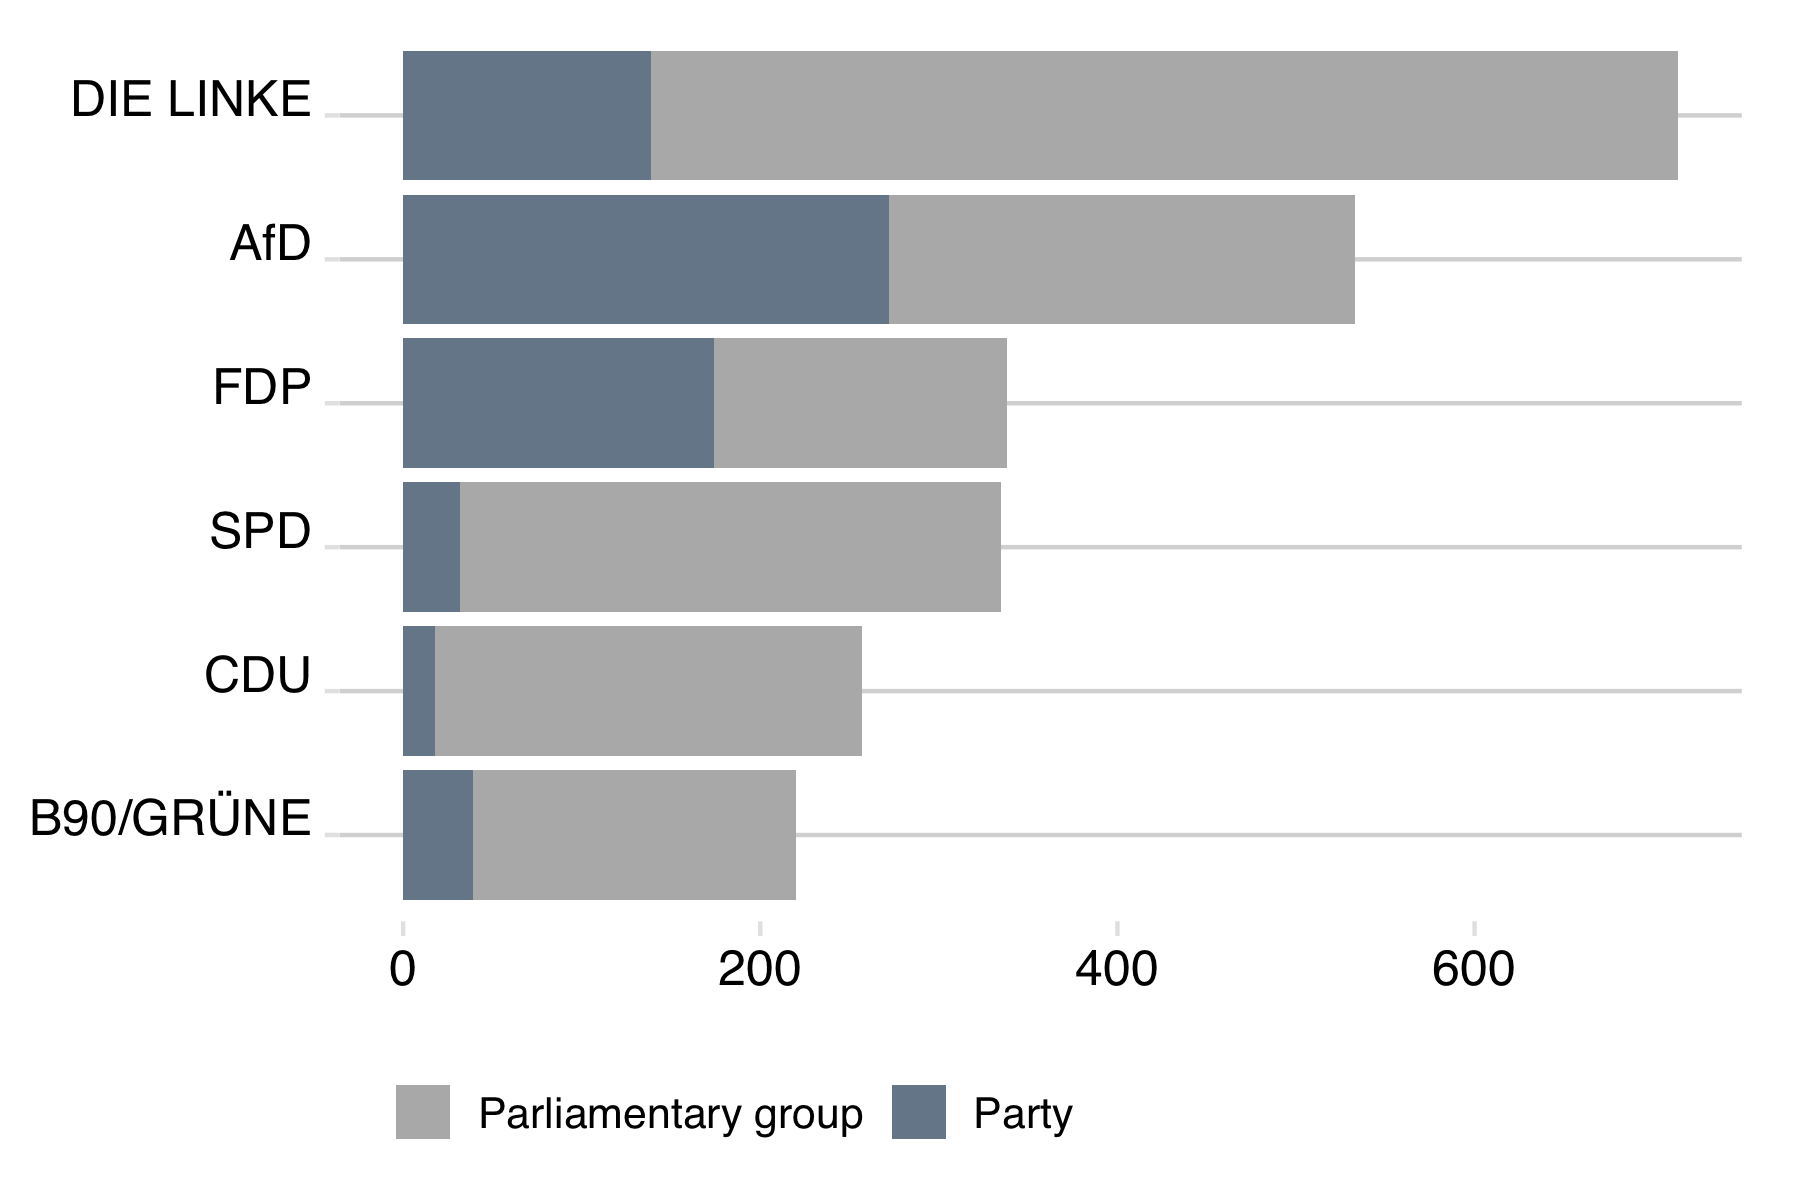
\includegraphics[width=\textwidth]{../figs/press_releases}
			\label{fig_press}
		\end{subfigure}
		\begin{subfigure}[normla]{0.59\textwidth}
			\caption{Text length}
			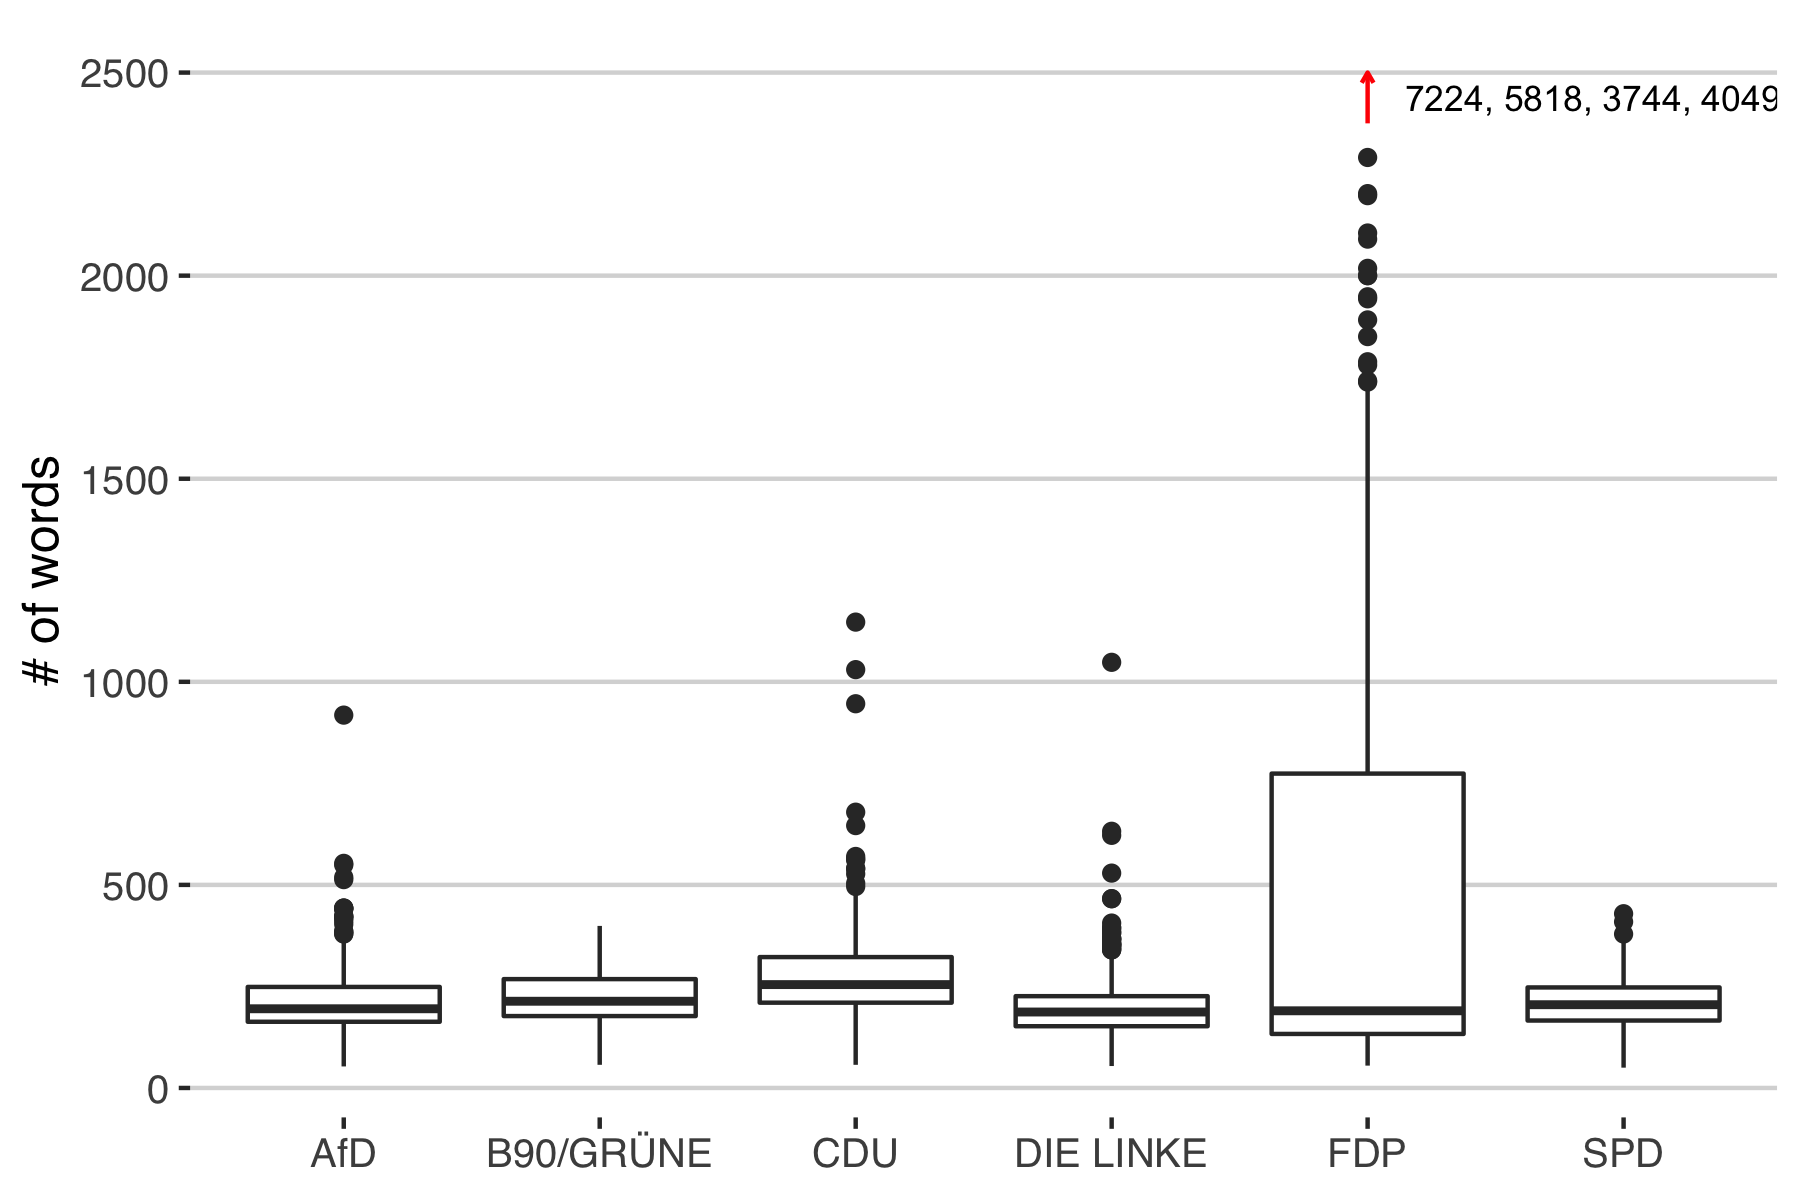
\includegraphics[width=\textwidth]{../figs/press_releases_textlength}
			\label{fig_press_textlength}
		\end{subfigure}
	\end{center}
\end{figure}


\subsection{News articles}\label{ch_news}

%% latex table generated in R 3.5.1 by xtable 1.8-3 package
% Sun Nov 11 21:36:13 2018
\begin{table}[ht]
\centering
\begin{tabular}{lrrr}
  \hline
medium & total\_articles & share & visits \\ 
  \hline
Bild.de & 3828 & 0.28 & 156867922 \\ 
  DIE WELT & 18663 & 0.14 & 52962285 \\ 
  FOCUS Online & 9235 & 0.22 & 68730873 \\ 
  SPIEGEL ONLINE & 5590 & 0.31 & 96139323 \\ 
  stern.de & 15804 & 0.15 & 18192672 \\ 
  tagesschau.de & 2261 & 0.41 & 75400000 \\ 
  ZEIT ONLINE & 5467 & 0.23 & 30600773 \\ 
   \hline
\end{tabular}
\caption{News sources used for the analysis} 
\end{table}


The data on news articles includes online articles from seven German news providers about domestic politics\footnote{Bild.de, DIE WELT, FOCUS ONLINE, SPIEGEL ONLINE, stern.de, ZEIT ONLINE, Tagesschau.de} dated from June 1, 2017 to March 1, 2018. First all online articles from the corresponding news websites are scraped using the Webhose.io API.\footnote{For more information see https://docs.webhose.io/v1.0/docs/getting-started. The scraping code was written in Python and can be made available on request.} In order to limit the analysis to articles on domestic politics, the articles are filtered using the url of the article. For example, the URL \textit{http://www.spiegel.de/politik/deutschland/christian-lindner-ukraine-kritisiert-fdp-chef-scharf-der-morgen-live-a-1161196.html} indicates that this article belongs thematically to 'politics' and 'deutschland' (Germany). After further cleaning processes (e.g. articles that only contain video content) the total sample size was 15,135. As shown in Figure \ref{fig_news_count} most articles were published by "Die Welt" and "tagesschau.de" has the smallest number of articles. Also in terms of text length is DIE WELT on top and tagesschau.de at the bottom. 

\begin{figure}[H]
	\begin{center}
	\caption{News articles}
		\begin{subfigure}[normla]{0.39\textwidth}
			\caption{Count}
			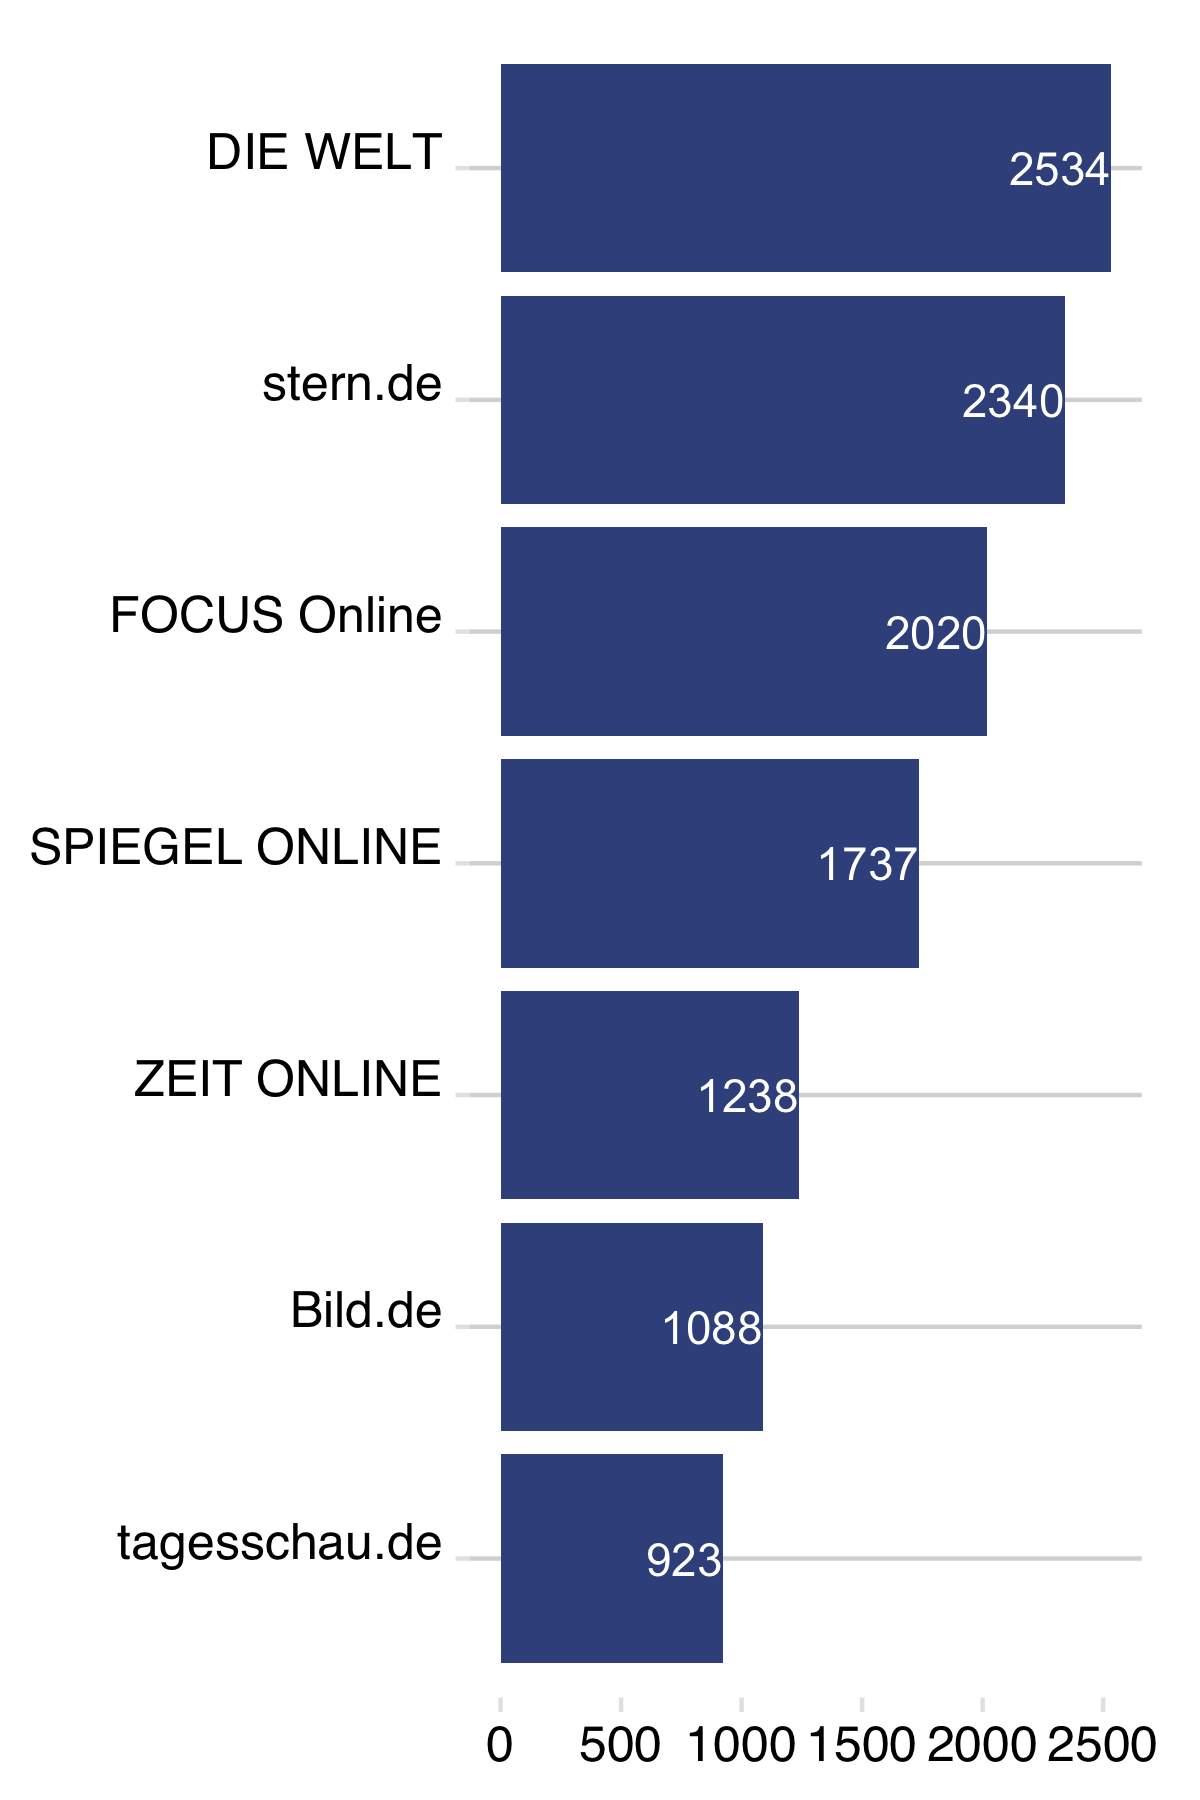
\includegraphics[width=\textwidth]{../figs/article_sum.png}
			\label{fig_news_count}
		\end{subfigure}
		\begin{subfigure}[normla]{0.59\textwidth}
			\caption{Text length}
			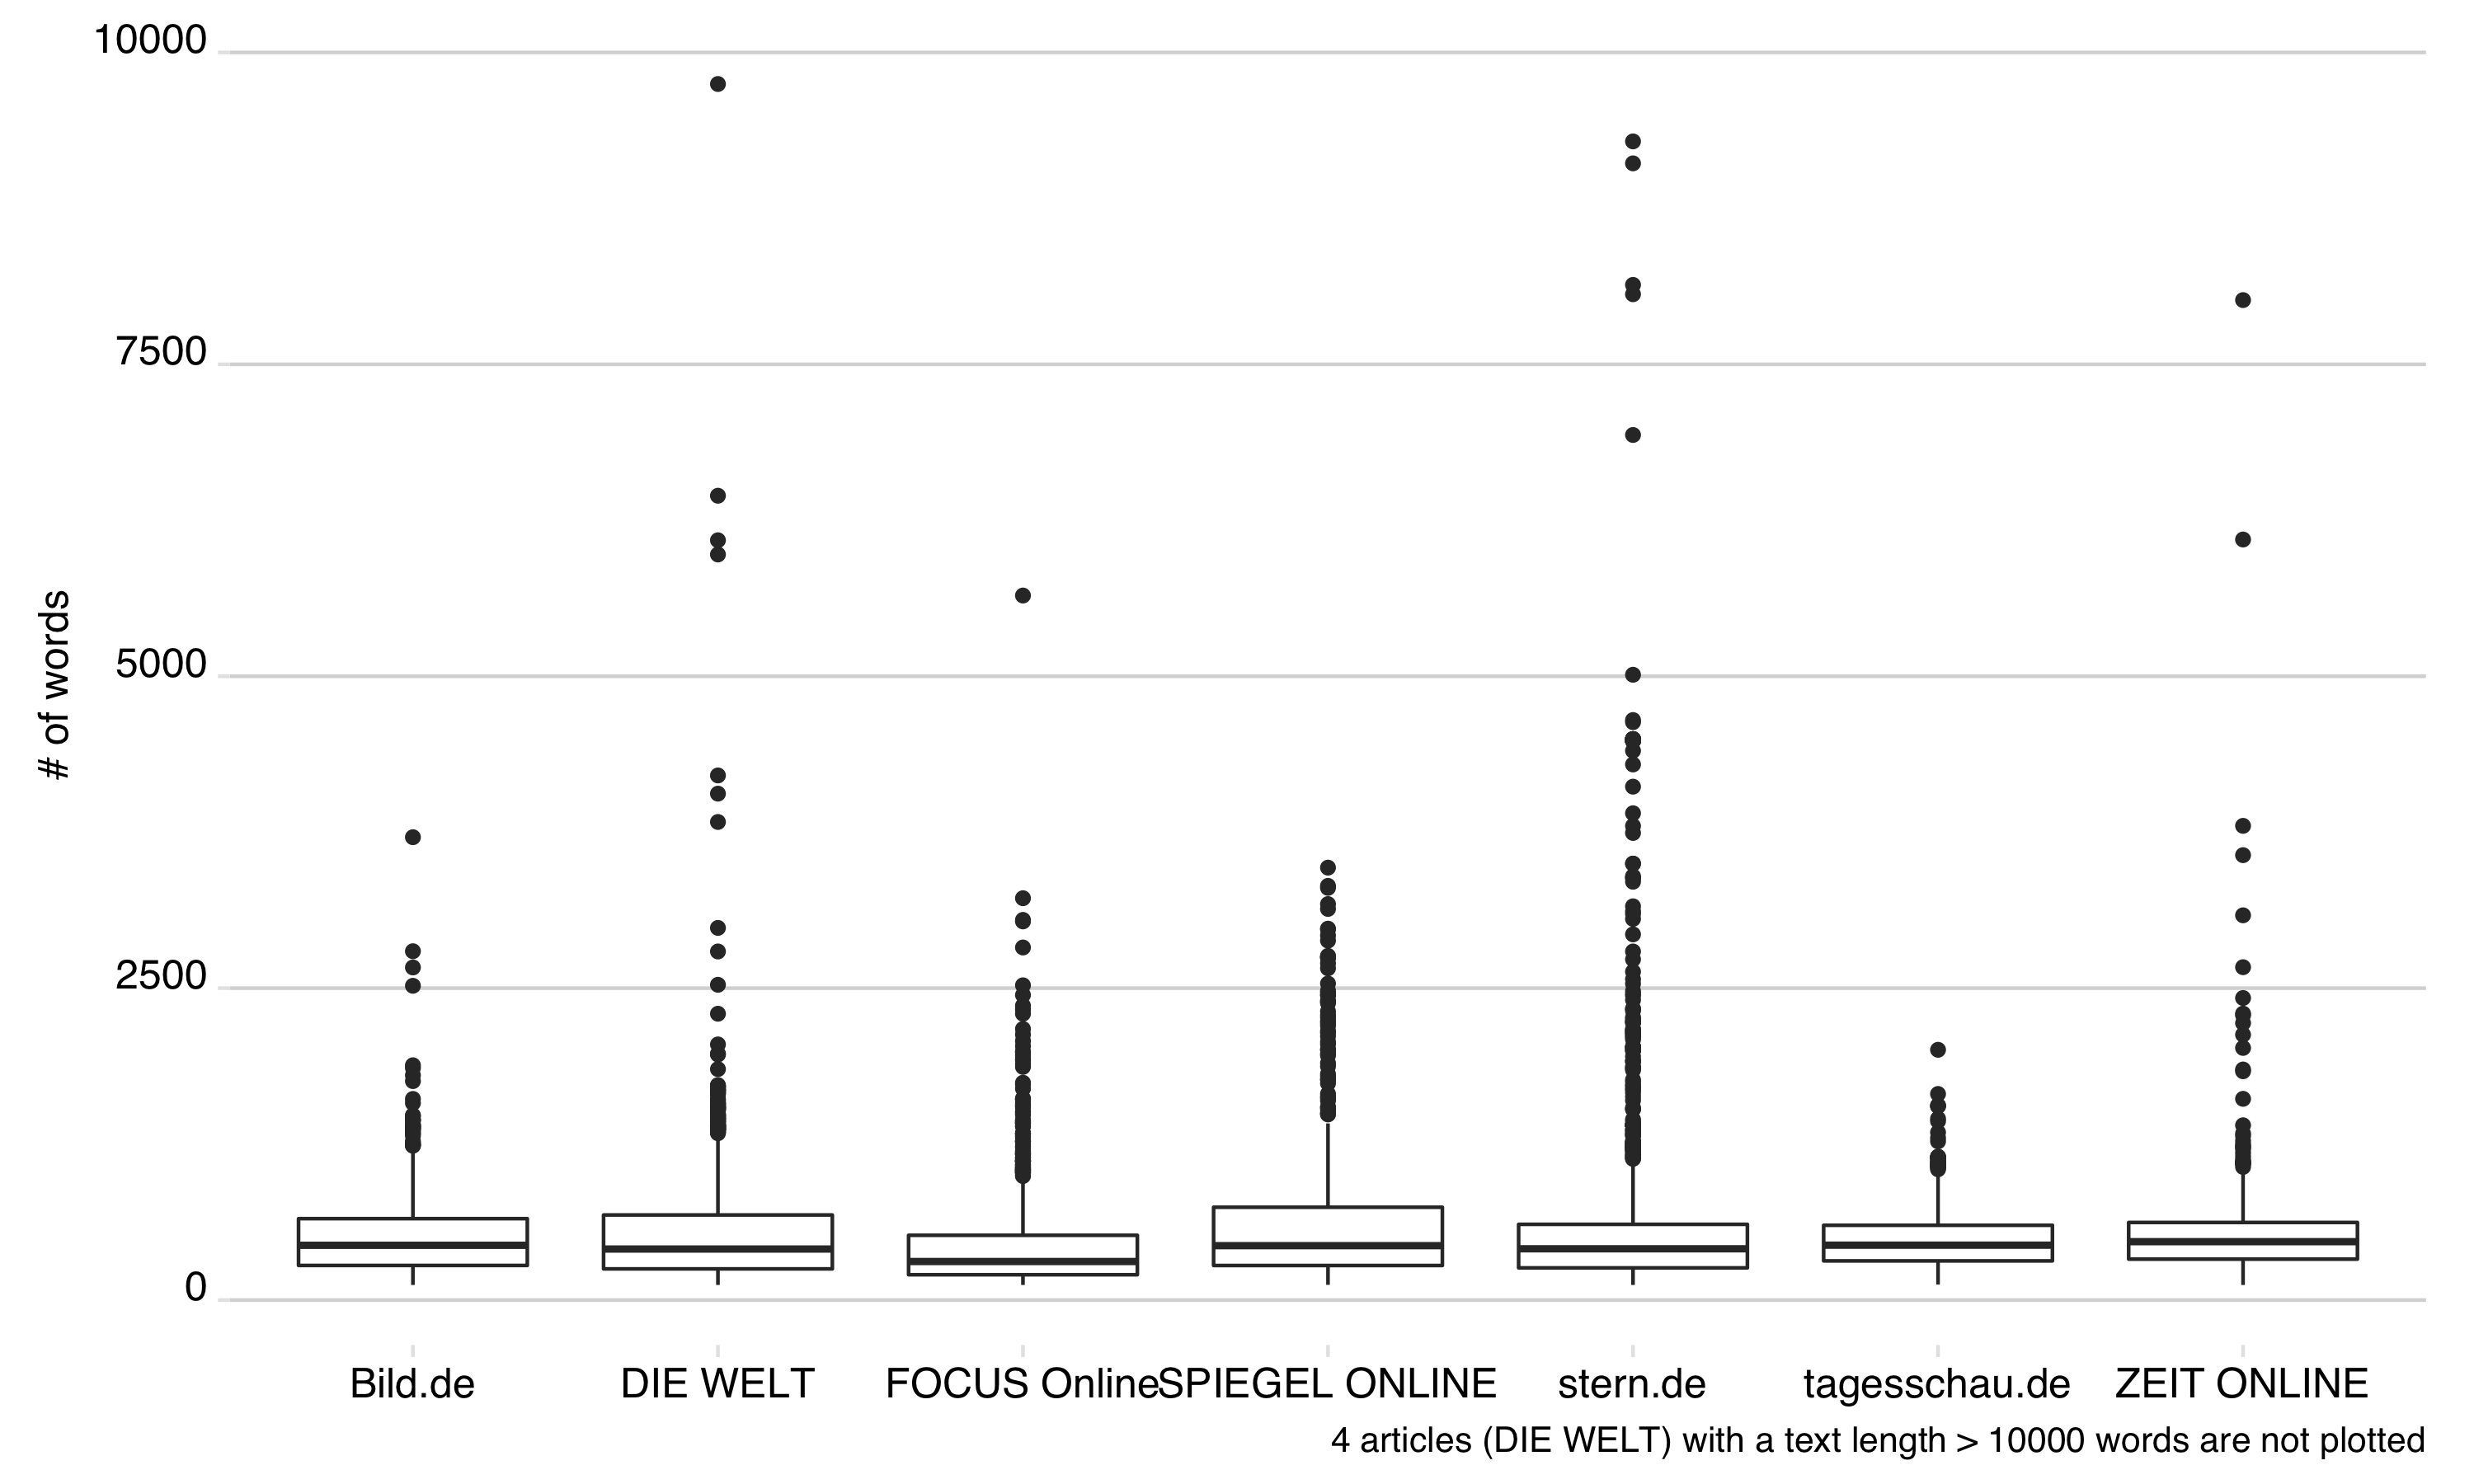
\includegraphics[width=\textwidth]{../figs/news_releases_textlength}
			\label{fig_length}
		\end{subfigure}
	\end{center}
\end{figure}

In order to get a deeper understanding of the extent to which the newspapers report about parties, the visibility of the individual parties in the news articles can be considered \citep{eberl_one_2017, junque_de_fortuny_media_2012, dalessio_media_2000}. The visibility of a party in a newspaper is defined as the number of news articles published by the newspaper on that party (e.g. articles that mention the name of the party), normalised on the total amount of articles by that newspaper in the corpus. A party is treated as visible in an article if the party itself is mentioned in an article (if an article contains the word "SPD", "CDU"/"CSU/Union","FDP","Grüne","AfD" or "Linke"). Obviously, due to their political or social relevance, not all parties receive the same amount of attention in the media. Thus, Figure \ref{fig_vis_absolute} shows that the major popular parties CDU and SPD are mentioned most frequently among all news providers, in contrast to the other parties. However, these external factors should influence all media outlets equally. To show the relative visibility of a party on a medium, the values are rescaled on an interval between 0 and 1 displayed in Figure \ref{fig_vis_relative}. 

- Bei Zeit online haben alle Parteien am meisten Sichtbarkeit / bei tagesschau.de am wenigsten
- Insgesamt scheint die Sichtbarkeit gleichmäßig verteilt zu sein, größere Unterschiede sind erkennbar bei Focus (wenig Grüne, mehr AfD) und Bild (weniger Linke, mehr FDP).

\begin{figure}[H]
	\begin{center}
	\caption{Visibility}
		\begin{subfigure}[normla]{0.42\textwidth}
			\caption{absolute values}
			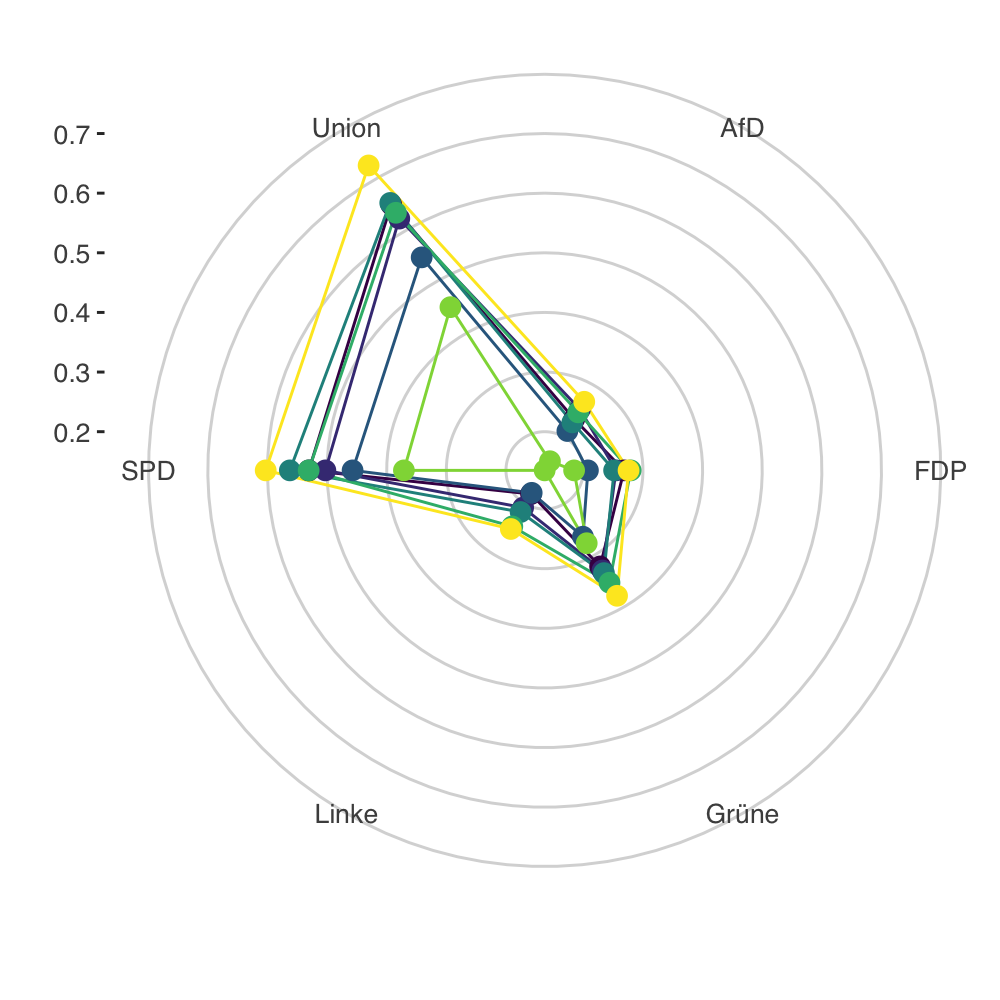
\includegraphics[width=\textwidth]{../figs/radar_vis}
			\label{fig_vis_absolute}
		\end{subfigure}
		\begin{subfigure}[normla]{0.52\textwidth}
			\caption{relative values}
			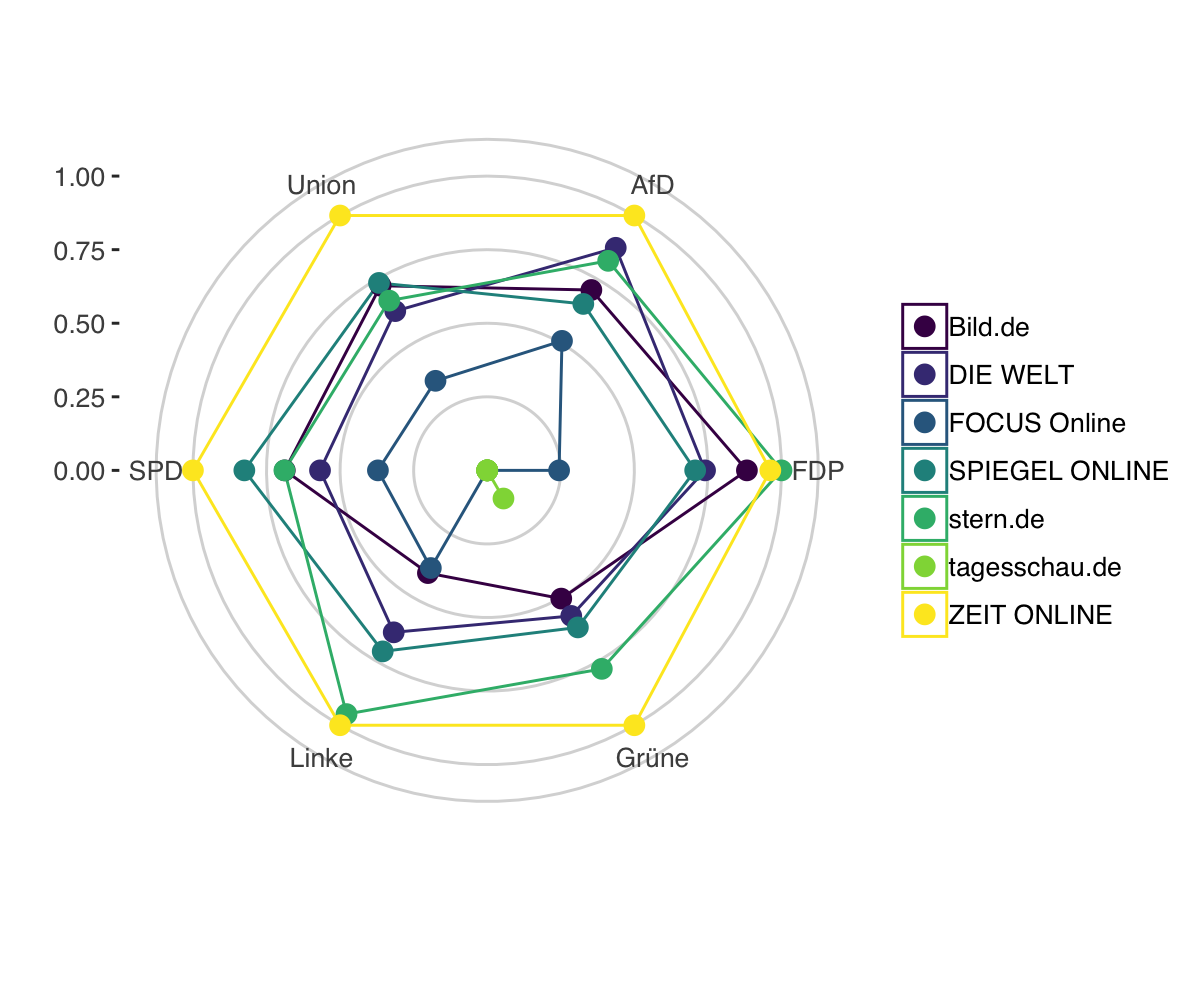
\includegraphics[width=\textwidth]{../figs/radar_vis_rescaled}
			\label{fig_vis_relative}
		\end{subfigure}
	\end{center}
\end{figure}

\subsection{Data preparation}

To use text as data for statistical analysis, different pre-processing steps have to be conducted. In fact, in order to use text as data and reduce the dimensionality to avoid unnecessary computational complexity and overfitting, pre-processsing the text is a central task in text mining \citep{gentzkow_text_2017, bholat_text_2015}. Intuitively the term frequency (tf) of a word is a measure of how important that word may be for the understanding of the text. To visualize these terms, word clouds are a commonly used technique in text mining as they translate the tf into the size of the term in the cloud. As can be seen in Figure \ref{fig_wordcloud1}, problems arise with words that are highly frequent. For example "die", or "der (eng. "the"), "und" (eng. "and"), and "ist" (eng. "is") are extremely common but unrelated to the quantity of interest. These terms, often called stop words \citep{gentzkow_text_2017}, are important to the grammatical structure of a text, but typically don't add any additional meaning and can therefore be neglected. 

To remove distorting words, the pre-defined stop word list from the Snowball project\footnote{http://snowball.tartarus.org/algorithms/german/stop.txt} is used together with a customized, domain-specific list of stop-words. Additionally punctuation character (e.g. ., ,, !, ?, etc.) and all numbers are removed from the data. A next step to reduce the dimensionality of text data is to apply an adequate stemming technique. Stemming is a process by which different morphological variants of a word are traced back to their common root. For example, "voting" and "vote" would be treated as two instances of the same token after the stemming process. There are many different techniques for the stemming process. I apply the widely used Porter-Stemmer algorithm, which is based on a set of shortening rules that are applied to a word until it has a minimum number of syllables.\footnote{https://tartarus.org/martin/PorterStemmer/} After completing these steps 63,360 unique terms were left in the vocabulary. The word clouds in Figure \ref{fig_wordcloud2} represent the most frequent words after pre-processing the text data. It becomes evident that the words "SPD", "CDU" and "AfD" among others seems to be highly frequent.  

\begin{figure}[H]
	\begin{center}
	\caption{Wordclouds}
		\begin{subfigure}[normla]{0.49\textwidth}
			\caption{before pre-processing}
			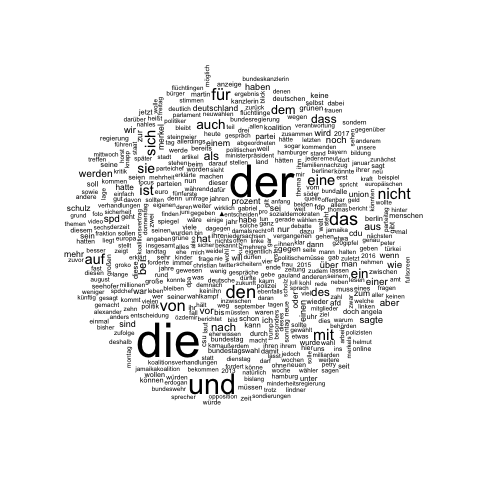
\includegraphics[width=\textwidth]{../figs/wordcloud}
			\label{fig_wordcloud1}
		\end{subfigure}
		\begin{subfigure}[normla]{0.49\textwidth}
			\caption{after pre-processing}
			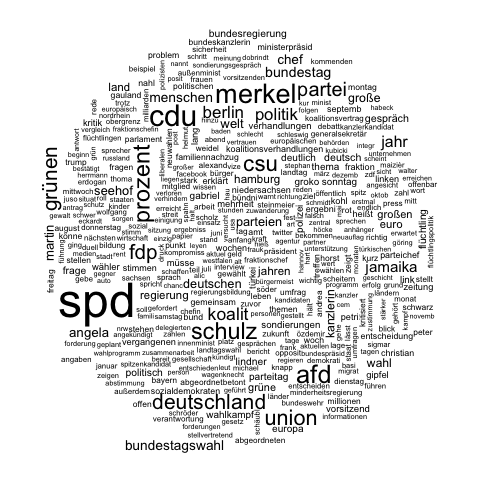
\includegraphics[width=\textwidth]{../figs/wordcloud_cleaned}
			\label{fig_wordcloud2}
		\end{subfigure}
	\end{center}
\end{figure}

% -------------------------
% Term-frequency by source
% -------------------------

\begin{figure}[H]
	\begin{center}
	\caption{Term frequency}
		\begin{subfigure}[normla]{0.57\textwidth}
			\caption{News articles}
			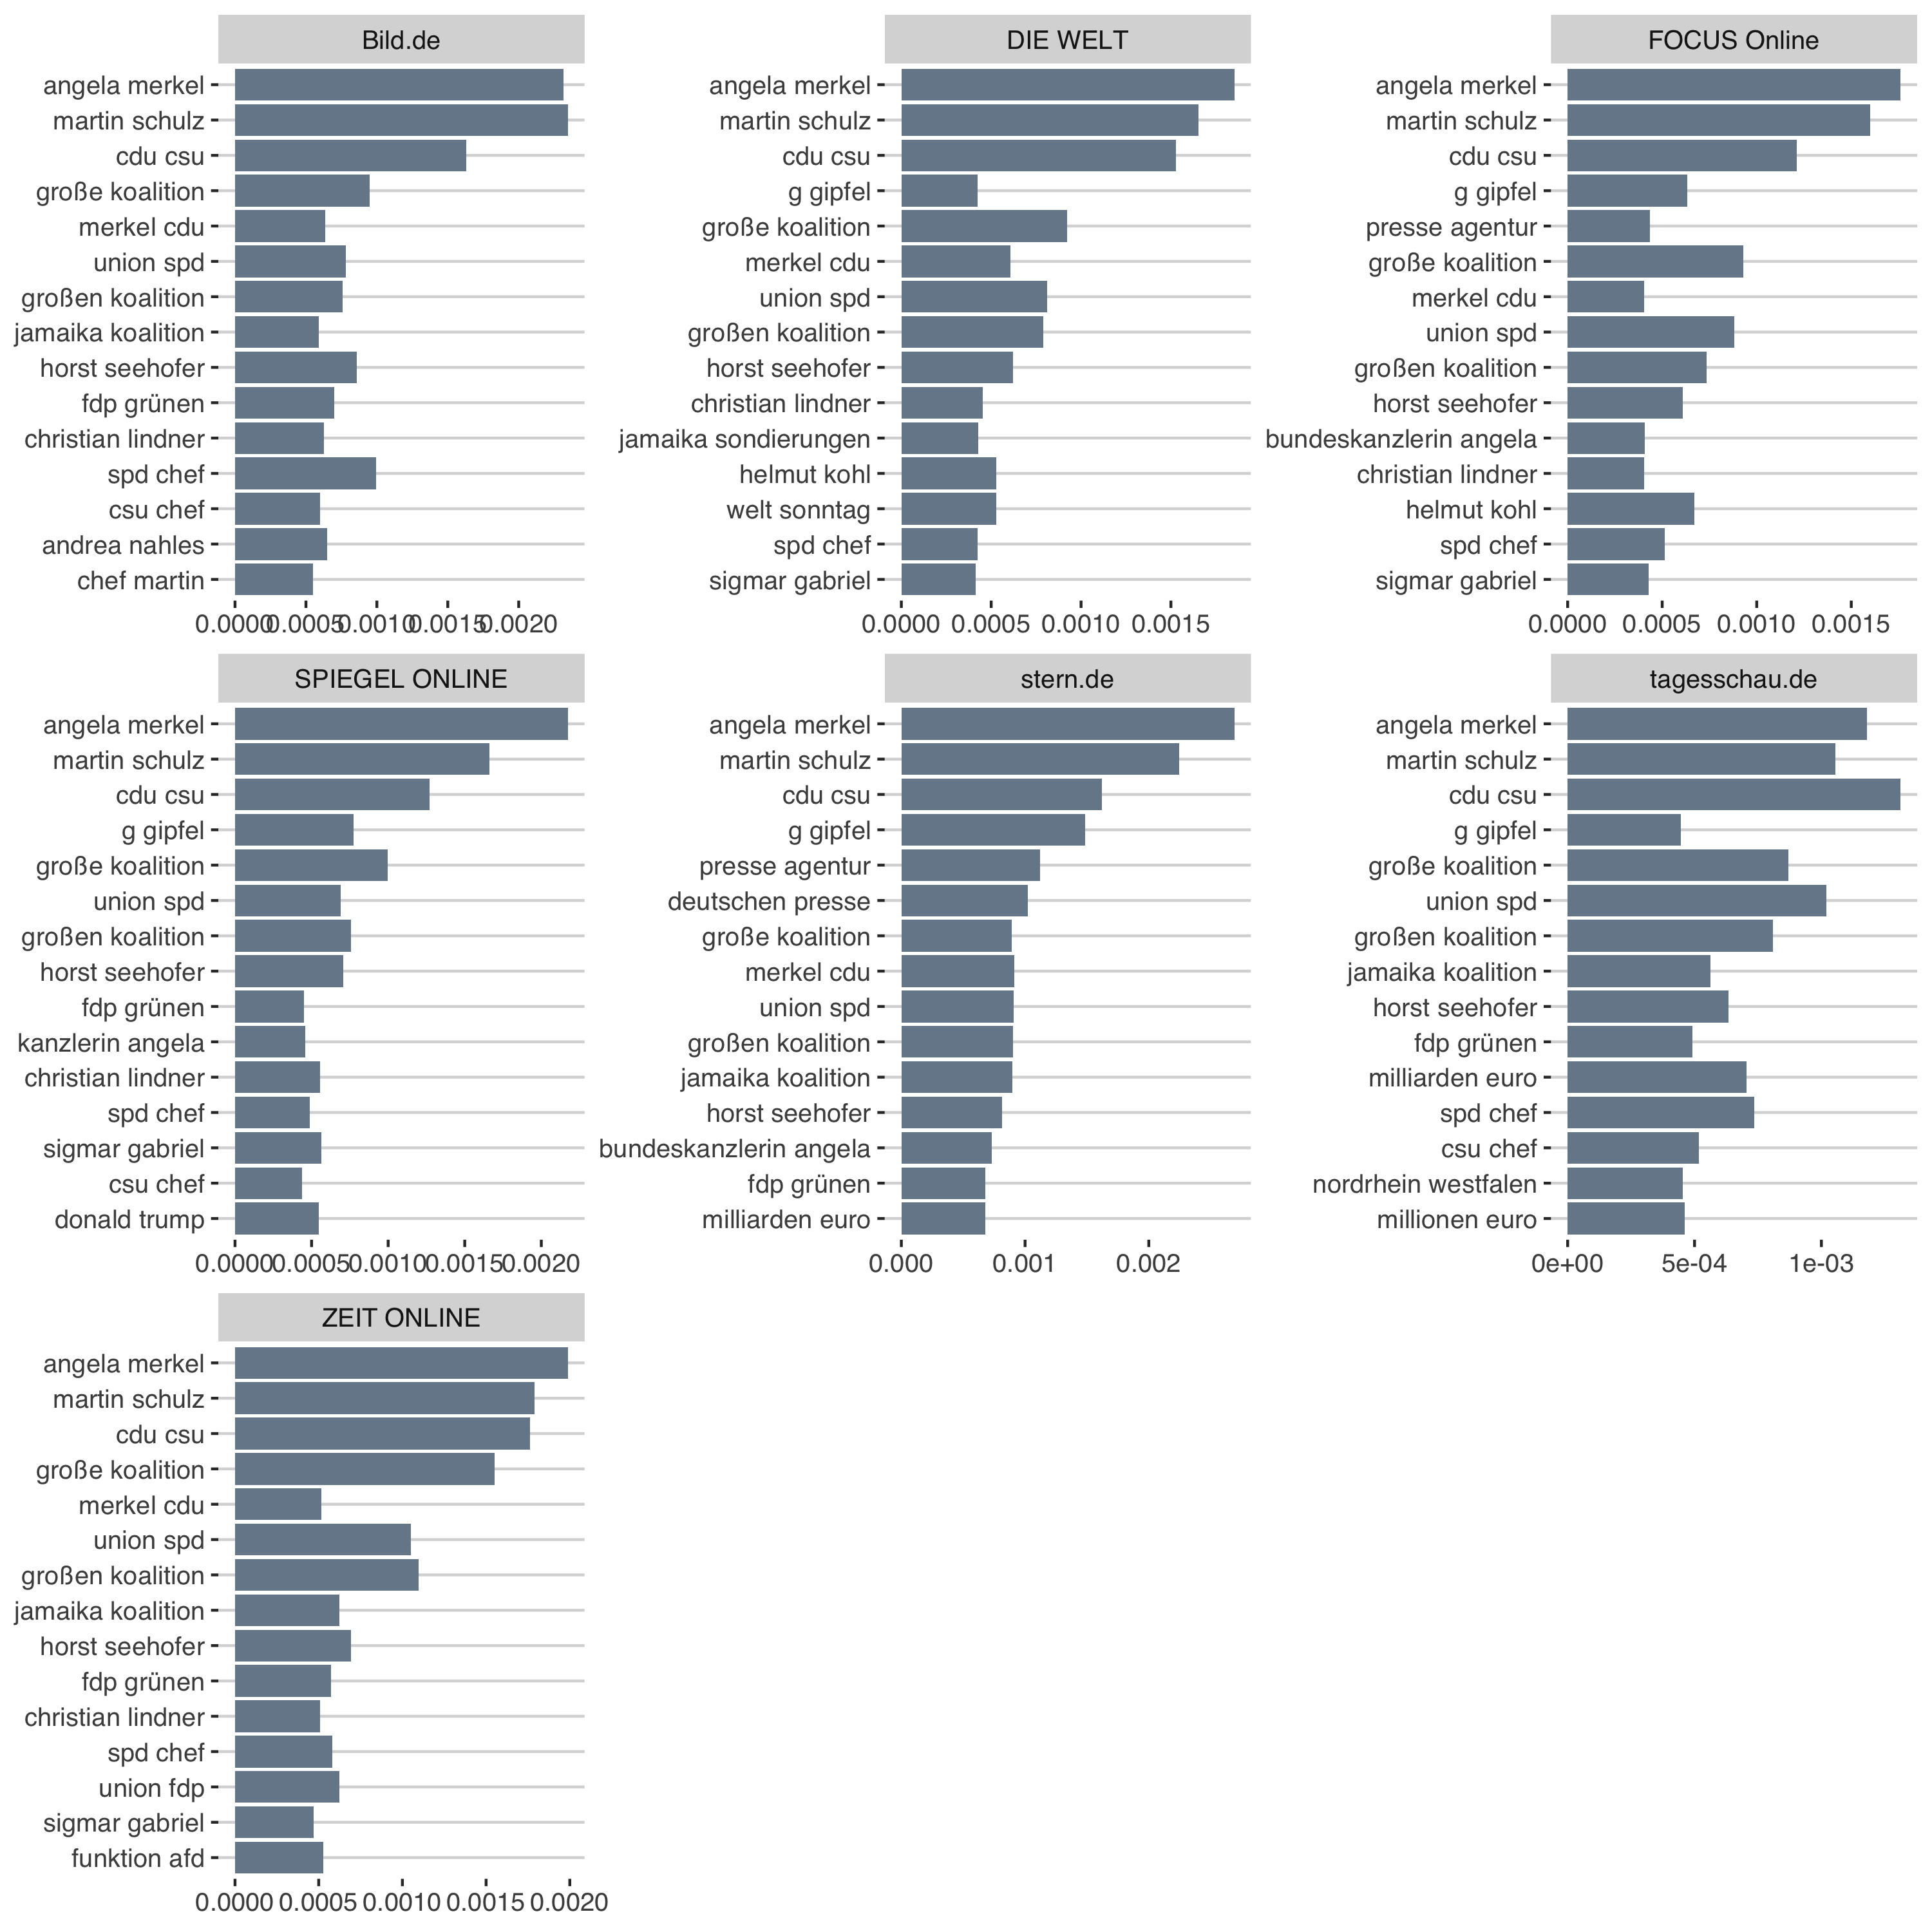
\includegraphics[width=\textwidth]{../figs/tf_bigrams_news}
			\label{fig_tf_news}
		\end{subfigure}
		\begin{subfigure}[normla]{0.38\textwidth}
			\caption{Press releases}
			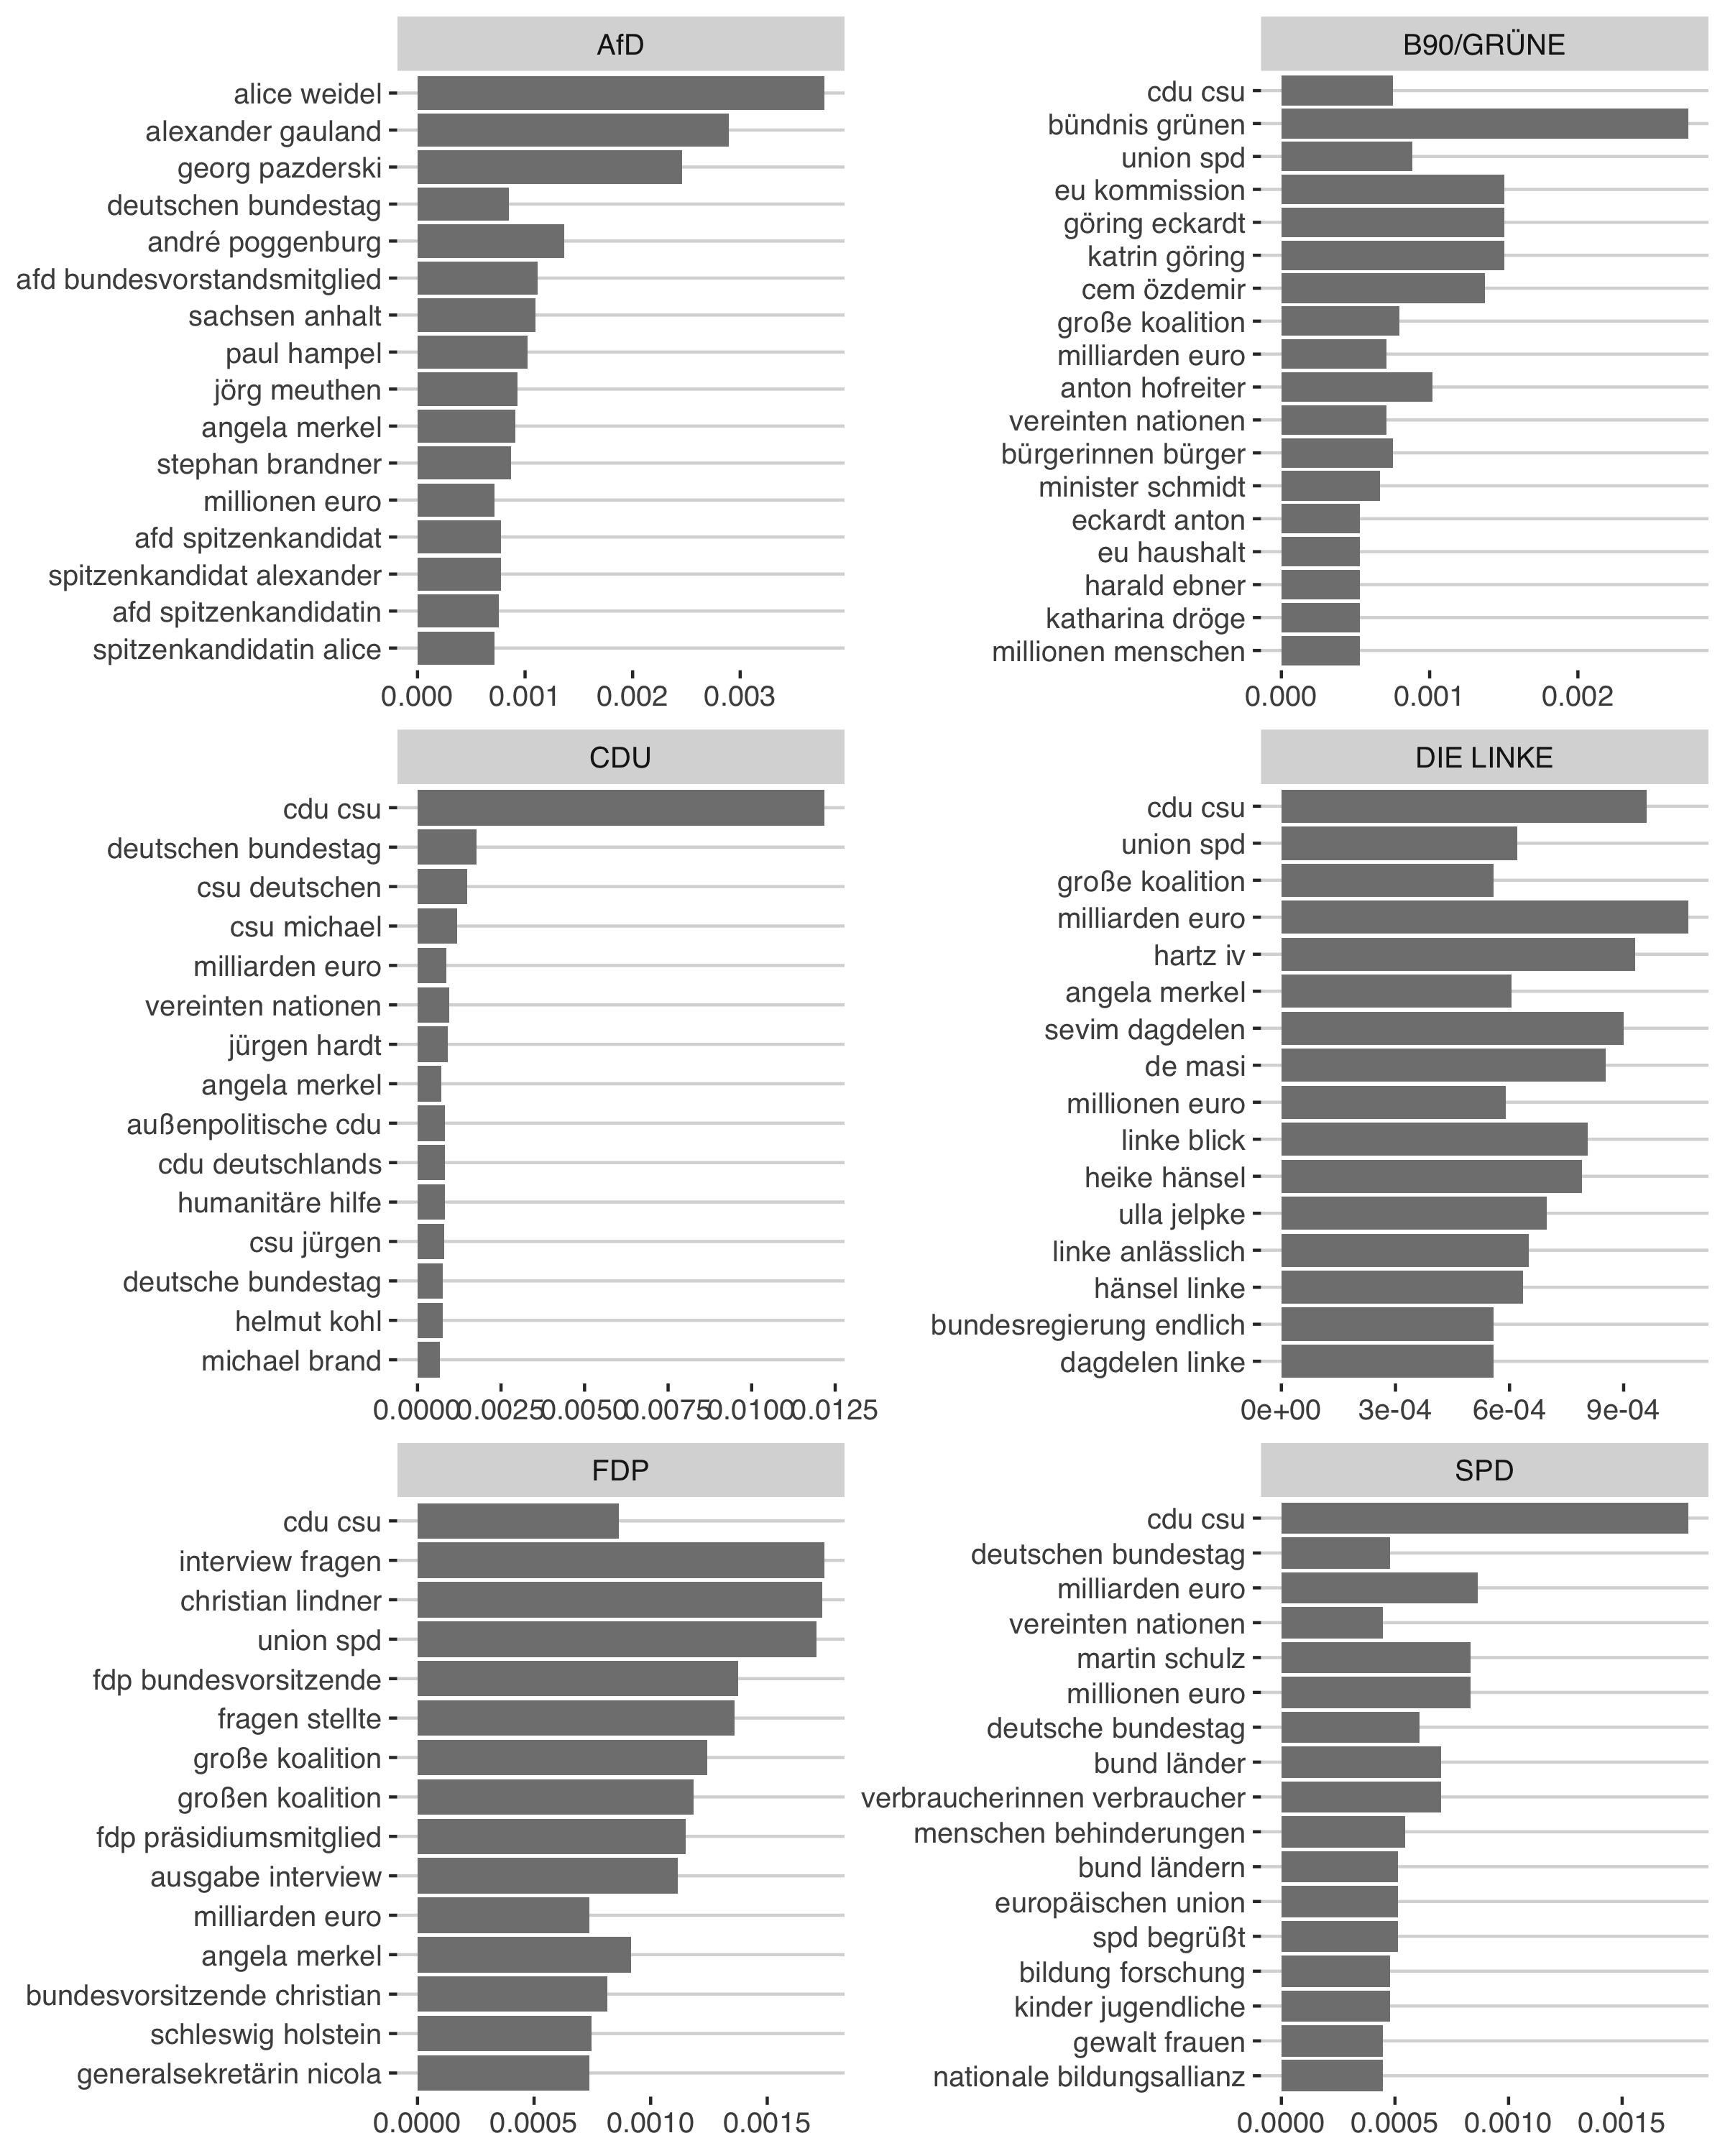
\includegraphics[width=\textwidth]{../figs/tf_bigrams_press}
			\label{fig_tf_press}
		\end{subfigure}
	\end{center}
\end{figure}

Figure \ref{fig_tf_news} and \ref{fig_tf_press} show the top 15 bigrams (pairs of two consecutive words) for each source in terms of frequency. While no obvious differences are visible for the news websites, the top words in the press releases make it easy to deduce the corresponding party. 

% --------------------
% Document-term-matrix
% --------------------
The next step is to divide the entire dataset into individual documents and to represent these documents as a finite list of unique terms. In this setting, each news article and each press release represents a document $d$, whereby each of these documents can be assigned to a news website or a party. The sum of all documents forms what is called the corpus. For each document $d \in \lbrace 1,...,D \rbrace$ the number of occurrences of term $v$ in document $d$ is computed, in order to obtain the count $x_{d,v}$, where each unique term in the corpus is indexed by some $v \in \lbrace 1,...,V \rbrace$ and where $V$ is the number of unique terms. The $D$ x $V$ matrix $\boldsymbol{X}$ of all such counts is called the document-term matrix. Each row in this matrix represents a document, where each entry in this row counts the occurrences of a unique term in that document. This representation is often referred to as the bag of words model \citep{gentzkow_text_2017}, since the order in which words are used within a document is disregarded.

\section{Measuring slant-index}\label{ch_method}

To discover the latent topics in the corpus of press releases (2.666) (see Section \ref{ch_press}) and news articles (15.135) (see Section \ref{ch_news}), a structural topic model (STM) developed by \citet{roberts_model_2016} is applied. The STM is an unsupervised machine learning approach that models topics as multinomial distributions of words (topical content) and documents as multinomial distributions of topics (topical prevalence of a document), allowing to incorporate external variables that effect both, topical content and topical prevalence. I estimate a model in which the source\footnote{Bild.de, DIE WELT, FOCUS ONLINE, SPIEGEL ONLINE, stern.de, ZEIT ONLINE, Tagesschau.de, CDU/CSU, SPD, AfD, FDP, B90/Die Grünen, DIE LINKE} of the document is included as a control for the topical prevalence, e.g. I assume that the possibility that a topic appears in a document depends on the source. Additionally, the type of source\footnote{press release or news article} is included as a control for the topical content, e.g. I assume that words used to describe the same topics differ between press releases and news articles. The results of the generative process of the STM are two posterior distributions: One for the topic prevalence in a document (what is the article or press release about?) and one for the content of a topic (what is the topic about?). The topic prevalence is used to calculate the agenda of each source as the mean over all documents that belong to that source. Subsequently the bivariate correlations between party agendas and the mediated party agendas in the online news are estimated. These correlations represent the agenda selectivity each party experiences in each media outlet. The higher the correlation, the more congruent both agendas are.  A more formale description of this process is described in Section \ref{ch_stm} and \ref{ch_agendacorrl}. In the last step I compare the agenda selectivity of each medium with the user preferences expressed in the Reuters Institute Digital News Survey (see Section \ref{ch_readerpref}). 

\subsection{Sentiment score}

To estimate the sentiment of each document a dictionary-based method is applied with the aim to measure the tone (or sentiment) of a document. The idea of a sentiment analysis is to determine the attitude of a writer toward the overall tonality of a document. To conduct such an analysis, a lists of words (dictionary) associated with a given emotion, such as negativity is pre-defined by the analyst. The document is then deconstructed into individual words and the frequencies of words contained in a given dictionary are calculated. 

Such lexical or "bag-of-words" approaches are widely presented in the finance literature to determine the effect of central banks' monetary policy communications on asset prices and real variables (\citet{nyman_news_2018} \citet{tetlock_giving_2007}, \citet{tetlock_more_2008}). \citet{hansen_shocking_2016} use a similar approach to measure "the two Ts" (Topic and tone). They explore the effects of FOMC (Federal Open Market Committee) statements on both market and real economic variables. To understand the latent topic of a statement, they apply LDA on a corpus of 142 FOMC decision statements split into sentences. They then measure how the central bank is talking about that topic, using a dictionary approach. To calculate their score, they subtract the negative words from the positive words und divide this by the number of total words of the statement. A similar score is used by \citet{nyman_news_2018}, who measure the effect of narratives and sentiment of financial market text-based data on developments in the financial system. They count the number of occurrences of excitement words and anxiety words and then scale these numbers by the total text size as measured by the number of characters.

The present paper uses a dictionary that lists words associated with positive and negative polarity weighted within the interval of $[-1; 1]$. SentimentWortschatz\footnote{SentiWS for short. available here: http://wortschatz.uni-leipzig.de/de/download}, is a publicly available German-language resource for sentiment analysis, opinion mining, etc.. The current version of SentiWS (v1.8b) contains 1,650 positive and 1,818 negative words, which sum up to 15,649 positive and 15,632 negative words including their inflections, respectively. 

The sentiment score for each document $d$ is calculated  based on the weighted polarity values for a word, defined on an interval between -1 and 1. The score is then calculated from the sum of the words in a document (which can be assigned to a word from the dictionary) divided by the total number of words in that document:
 
\begin{equation}
	\text{SentScore}_d = \frac{|\text{positive polarity score}_d| - |\text{negative polarity score}_d|}{|\text{TotalWords}_d|}
\end{equation}

\subsection{Structural topic model}\label{ch_stm}

To find out the latent topics of each document, a structural topic model (STM) is estimated. In general, topic models formalize the idea that documents are formed by hidden variables (topics) that generate correlations among observed terms. They belong to the group of unsupervised generative models, meaning that the true attributes (topics) cannot be observed. The STM developed by \citet{roberts_model_2016} is a recent extension of the standard topic modelling technique, labeled as latent Dirichlet allocation (LDA), which refers to the Bayesian model in \citet{blei_latent_2003} that treats each word in a topic and each topic in a document as generated from a Dirichlet - distributed prior.\footnote{See also \citet{griffiths_probabilistic_2002}, \citet{griffiths_finding_2004} and \citet{hofmann_probabilistic_1999}}. 

 One crucial assumption to be made for such models is the number of topics ($K$) that occur over the entire corpus. The underlying idea for these models suggests that each individual topic $k$ potentially contains all of the unique terms within the vocabulary $V$ with different probability. Therefore, each topic $k$ can be represented as a probability vector $\phi_k$ over all unique terms $V$. Simultaneously, each individual document $d$ in the corpus can be represented as a probability distribution $\theta_d$ over the $K$ topics.

The difference between the widely used LDA and the STM approaches lies in how the posterior distributions ($\theta$ and $\phi$) are determined. LDA assumes that $\theta ~ \text{Dirichlet}(\alpha)$ and $\phi ~ \text{Dirichlet}(\beta)$, where $\alpha$ and $\beta$ are fitted with the model. While for STM, the prior distributions for $\theta$ and $\phi$ depend on document-level covariates (e.g. the author or date of a document). For this purpose, the the STM specifies two design matrices of covariates ($X$ and $Z$), where each line defines a vector of covariates for a specific document. In $X$, the covariates for topic prevalence are given, so that the probability of a topic for each document varies according to $X$, rather than resulting from a single common prior. The same applies to $Z$, in which the covariates for the word distribution within a topic are specified. The underlying data generating process to generate each individual word $w_{d,n}$ in a document $d$ for the $n^{th}$ word-position can be described as follows:\footnote{A more detailed description of the generative process of the STM can be found in section \ref{a_generativeProcess}}

\begin{itemize}
	\item for each document $i$, draw its distribution of topics $\theta_d$ depending on the metadata included in the model defined in $X$; 
	\item for each topic $k$, draw its distribution of words $\phi_k$ depending on the metadata included in the model defined in $Z$;
	\item for each word $n$, draw its topic $z_n$ based on $\theta_i$;
	\item for each word word $n$, draw the term distribution for the selected topic $\phi_{z_{d,n}}$.
\end{itemize}

% ----------------------
% Model Selection
% ----------------------
Inference of mixed-membership models, such as the one applied in this paper, has been a thread of research in applied statistics \citep{blei_latent_2003, erosheva_mixed-membership_2004, braun_variational_2010}. Topic models are usually imprecise as the function to be optimized has multiple modes, such that the model results can be sensitive to the starting values (e.g. the number of topics). Since an ex ante valuation of a model is hardly possible, I compute a variety of different models and compare their posterior probability. This enables me to check how results vary for different model solution \citep{roberts_navigating_2016}. I then cross-checked some subset of assigned topic distributions to evaluate whether the estimates align with the concept of interest \citep{gentzkow_text_2017}. These manual audits are applied together with numeric optimization based on the topic coherence measure suggested by \citet{mimno_optimizing_2011}. 

This process revealed that a model with 50 topics best reflects the structure in the corpus. Furthermore, the source of a document\footnote{Each party as well as each media outlet represent one source.} is used as covariate in the topic prevalence. In other words, I assume that the probability distribution of topics for a specific document is influenced by the source of that document. Additionally the type of that source (news website or party) is used as a covariate for the term frequency as I assume that the words used for the same topic differ between news articles or press releases.  


% -----------------------------
% ---- Agenda correlation -----
% -----------------------------
\subsection{Weighted topic correlation}\label{ch_agendacorrl}

The process described in \ref{ch_stm} generates two different kinds of posterior distributions that can be represented as the following matrices: 

\begin{enumerate}
	\item $\Phi_c$ is a $K$-by-$V$ matrix (where $K=$ number of topics and $V=$ vocabulary or unique terms), where the entry $\phi_{k,v,c}$ can be interpreted as the probability of observing the $v$-th word in topic $k$ for the covariate level $c$ (type of source: press release or news website). 
	\item $\Theta$ is a $D$-by-$K$ matrix (where $D=$ number of documents and $K=$ number of topics), where the entry $\theta_{d,k}$ can be interpreted as the proportion of words in document $d$ which arise from topic $k$, or rather as the probability that document $d$ deals about topic $k$. 
\end{enumerate}

To combine the sentiment value with the topic probability of each document, the sentiment score is multiplied with the $k$x$1$ vector for each document. Subsequently, to calculate the average topic sentiment for a source $s$, the mean value of all documents belonging to source $s$ is calculated. This results in a $k$x$1$ vector representing the mean distributions $\bar{ \theta_{s} }$ of this source, weighted by the sentiment scores:

\begin{equation}
	\bar{ \theta_{s} } =
	\begin{bmatrix} 
	\bar{ \theta_{1} } \\
	. \\
	. \\
	\bar{ \theta_{k} } \\
	\end{bmatrix}
\end{equation} 


On the basis of these values, the bivariate Pearson correlation coefficients are calculated for each pair of media outlet and party  on a monthly basis. The higher the correlation coefficient, the higher the slant index for a party in a media outlet.

% ---------------------- 
% ------- Results 
% ---------------------- %

\section{Results}

\subsection{Sentiment}

- Figure \ref{fig_sentiment} shows the aggregated sentiment value for each source. Dashed line shows the median value. 
- overall: all values are negative or 0 (CDU).
- parties: higher sentiment variance. DIE LINKE is most negative, CDU most positive
- media: FOCUS Online most negative, stern.de most positive. 

\begin{figure}[H]
\begin{center}
	\caption{Sentiment score }
	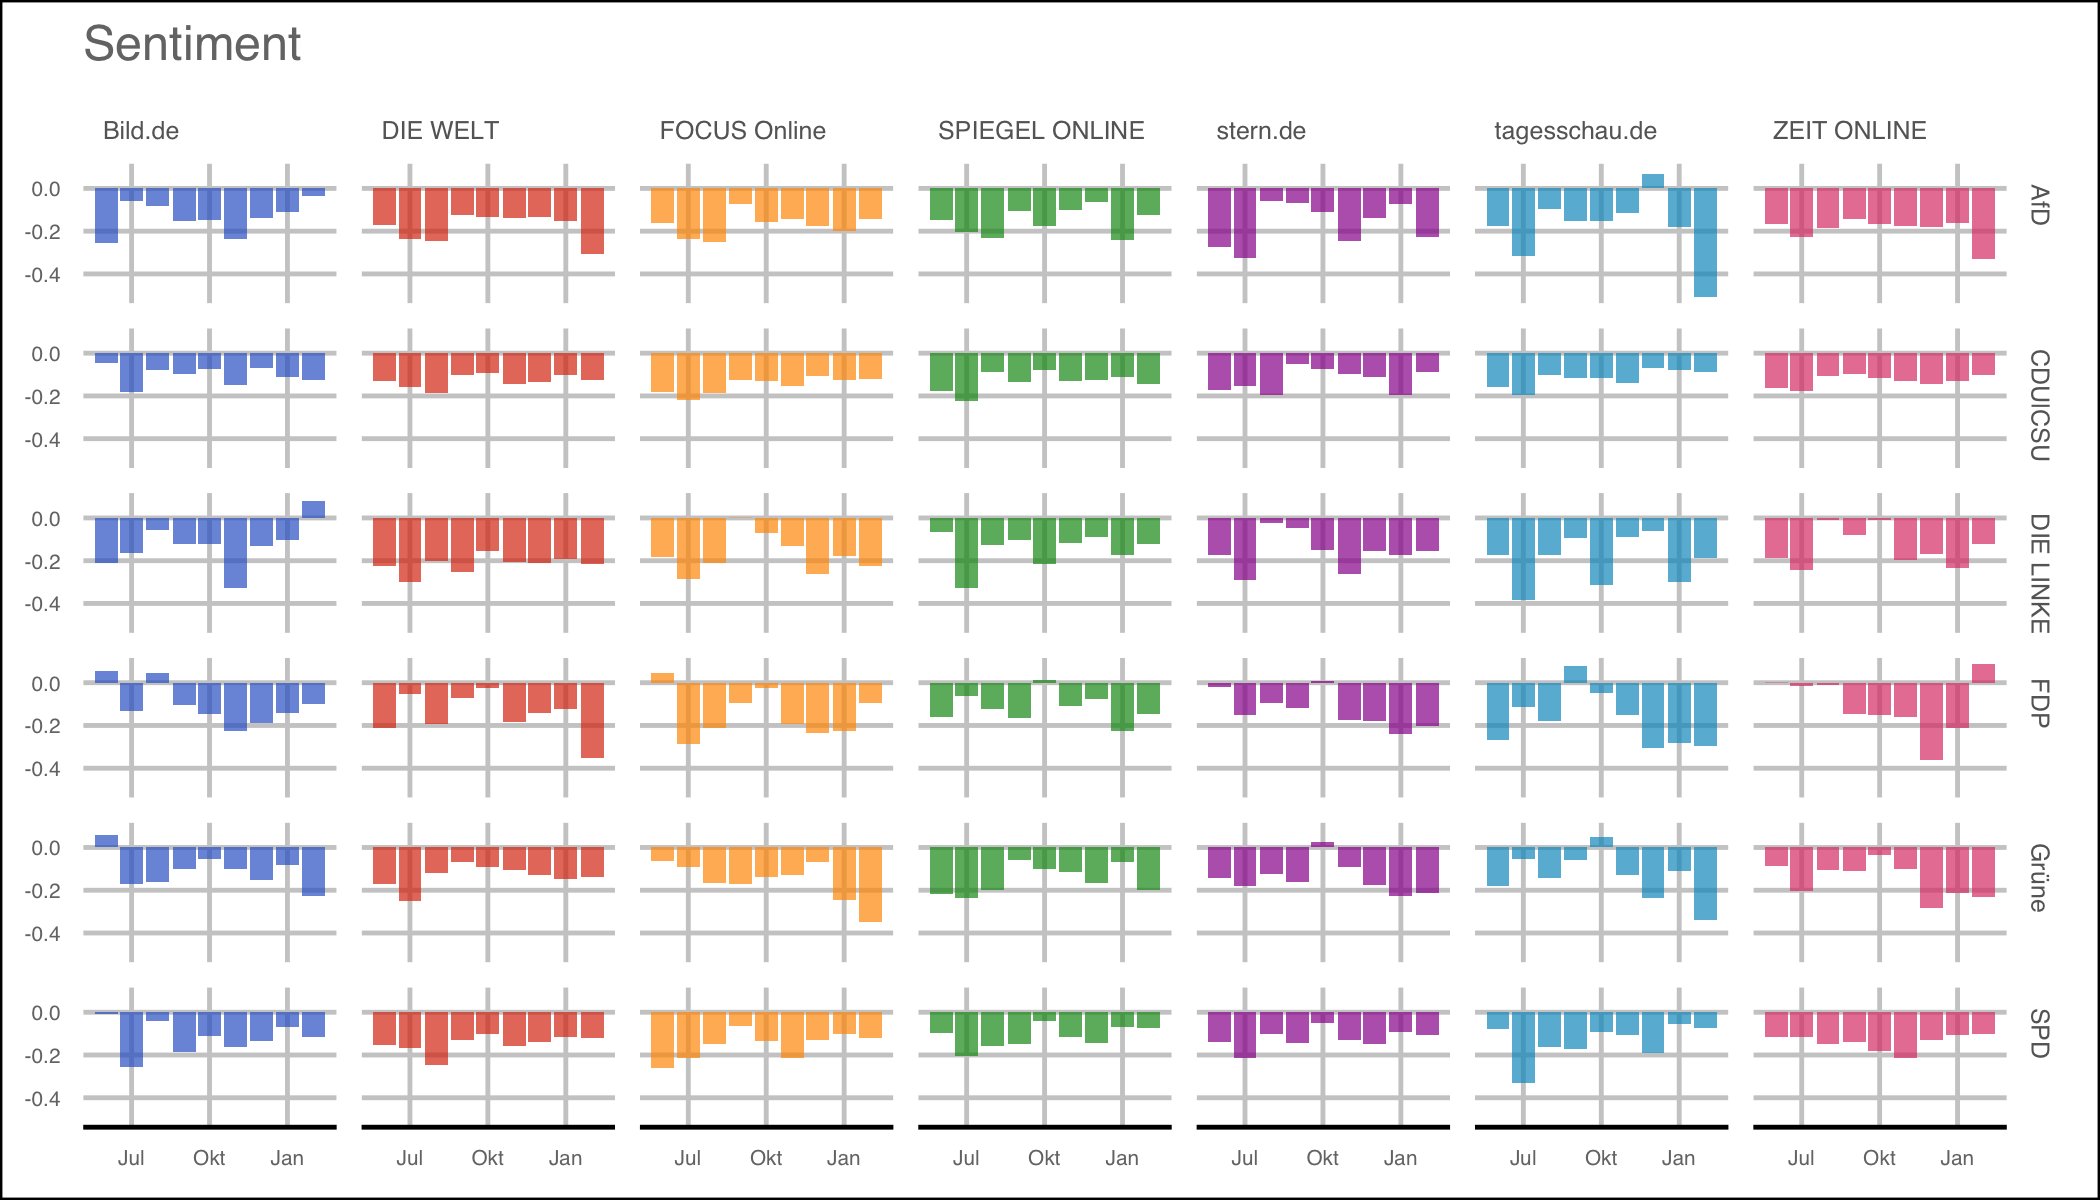
\includegraphics[width=.8\textwidth]{../figs/sentiment}
	\label{fig_sentiment}
	\end{center}
\end{figure}



\subsection{Topics} 

As stated above, the generative process of the STM results in a matrix $\Phi_c$ representing the probability of words in each topic. The most frequent words in each topic help to understand what each topic is about. Since the type of source is included as a covariate in the model specification, the result consists of two matrices (one for each covariate level $c$). It is therefore important to check the different word-distributions for each topic. The following Figure shows the 20 most frequent words for the first 3 topics separated between the covariate levels "news article" and "press release".\footnote{See \ref{a_labels} for a table of the most frequent words for each topic.}.

\begin{figure}[H]
	\caption{Most frequent terms}
	\begin{center}
		\begin{subfigure}[normla]{0.3\textwidth}
			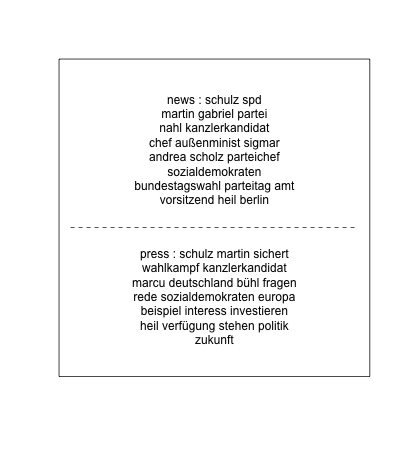
\includegraphics[width=\textwidth]{../figs/topiclabel/topic_label1}
			\caption{Topic 1}
		\end{subfigure}
		\begin{subfigure}[normla]{0.3\textwidth}
			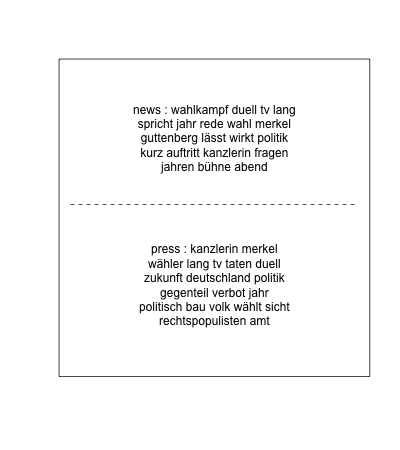
\includegraphics[width=\textwidth]{../figs/topiclabel/topic_label2}
			\caption{Topic 2}
		\end{subfigure}
		\begin{subfigure}[normla]{0.3\textwidth}
			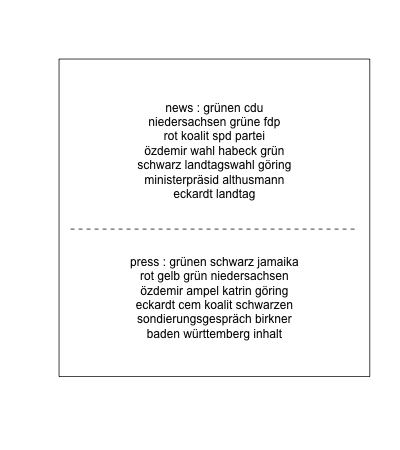
\includegraphics[width=\textwidth]{../figs/topiclabel/topic_label3}
			\caption{Topic 3}
		\end{subfigure}
	\end{center}
\end{figure}

The second posterior distribution from the STM results in a topic distribution $\theta_d$ for each document $d$ over all topics $k$.  An example of this distribution is shown in Figure \ref{fig_doc_topic_distr}.

\begin{figure}[H]
\begin{center}
	\caption{Topic frequency}
	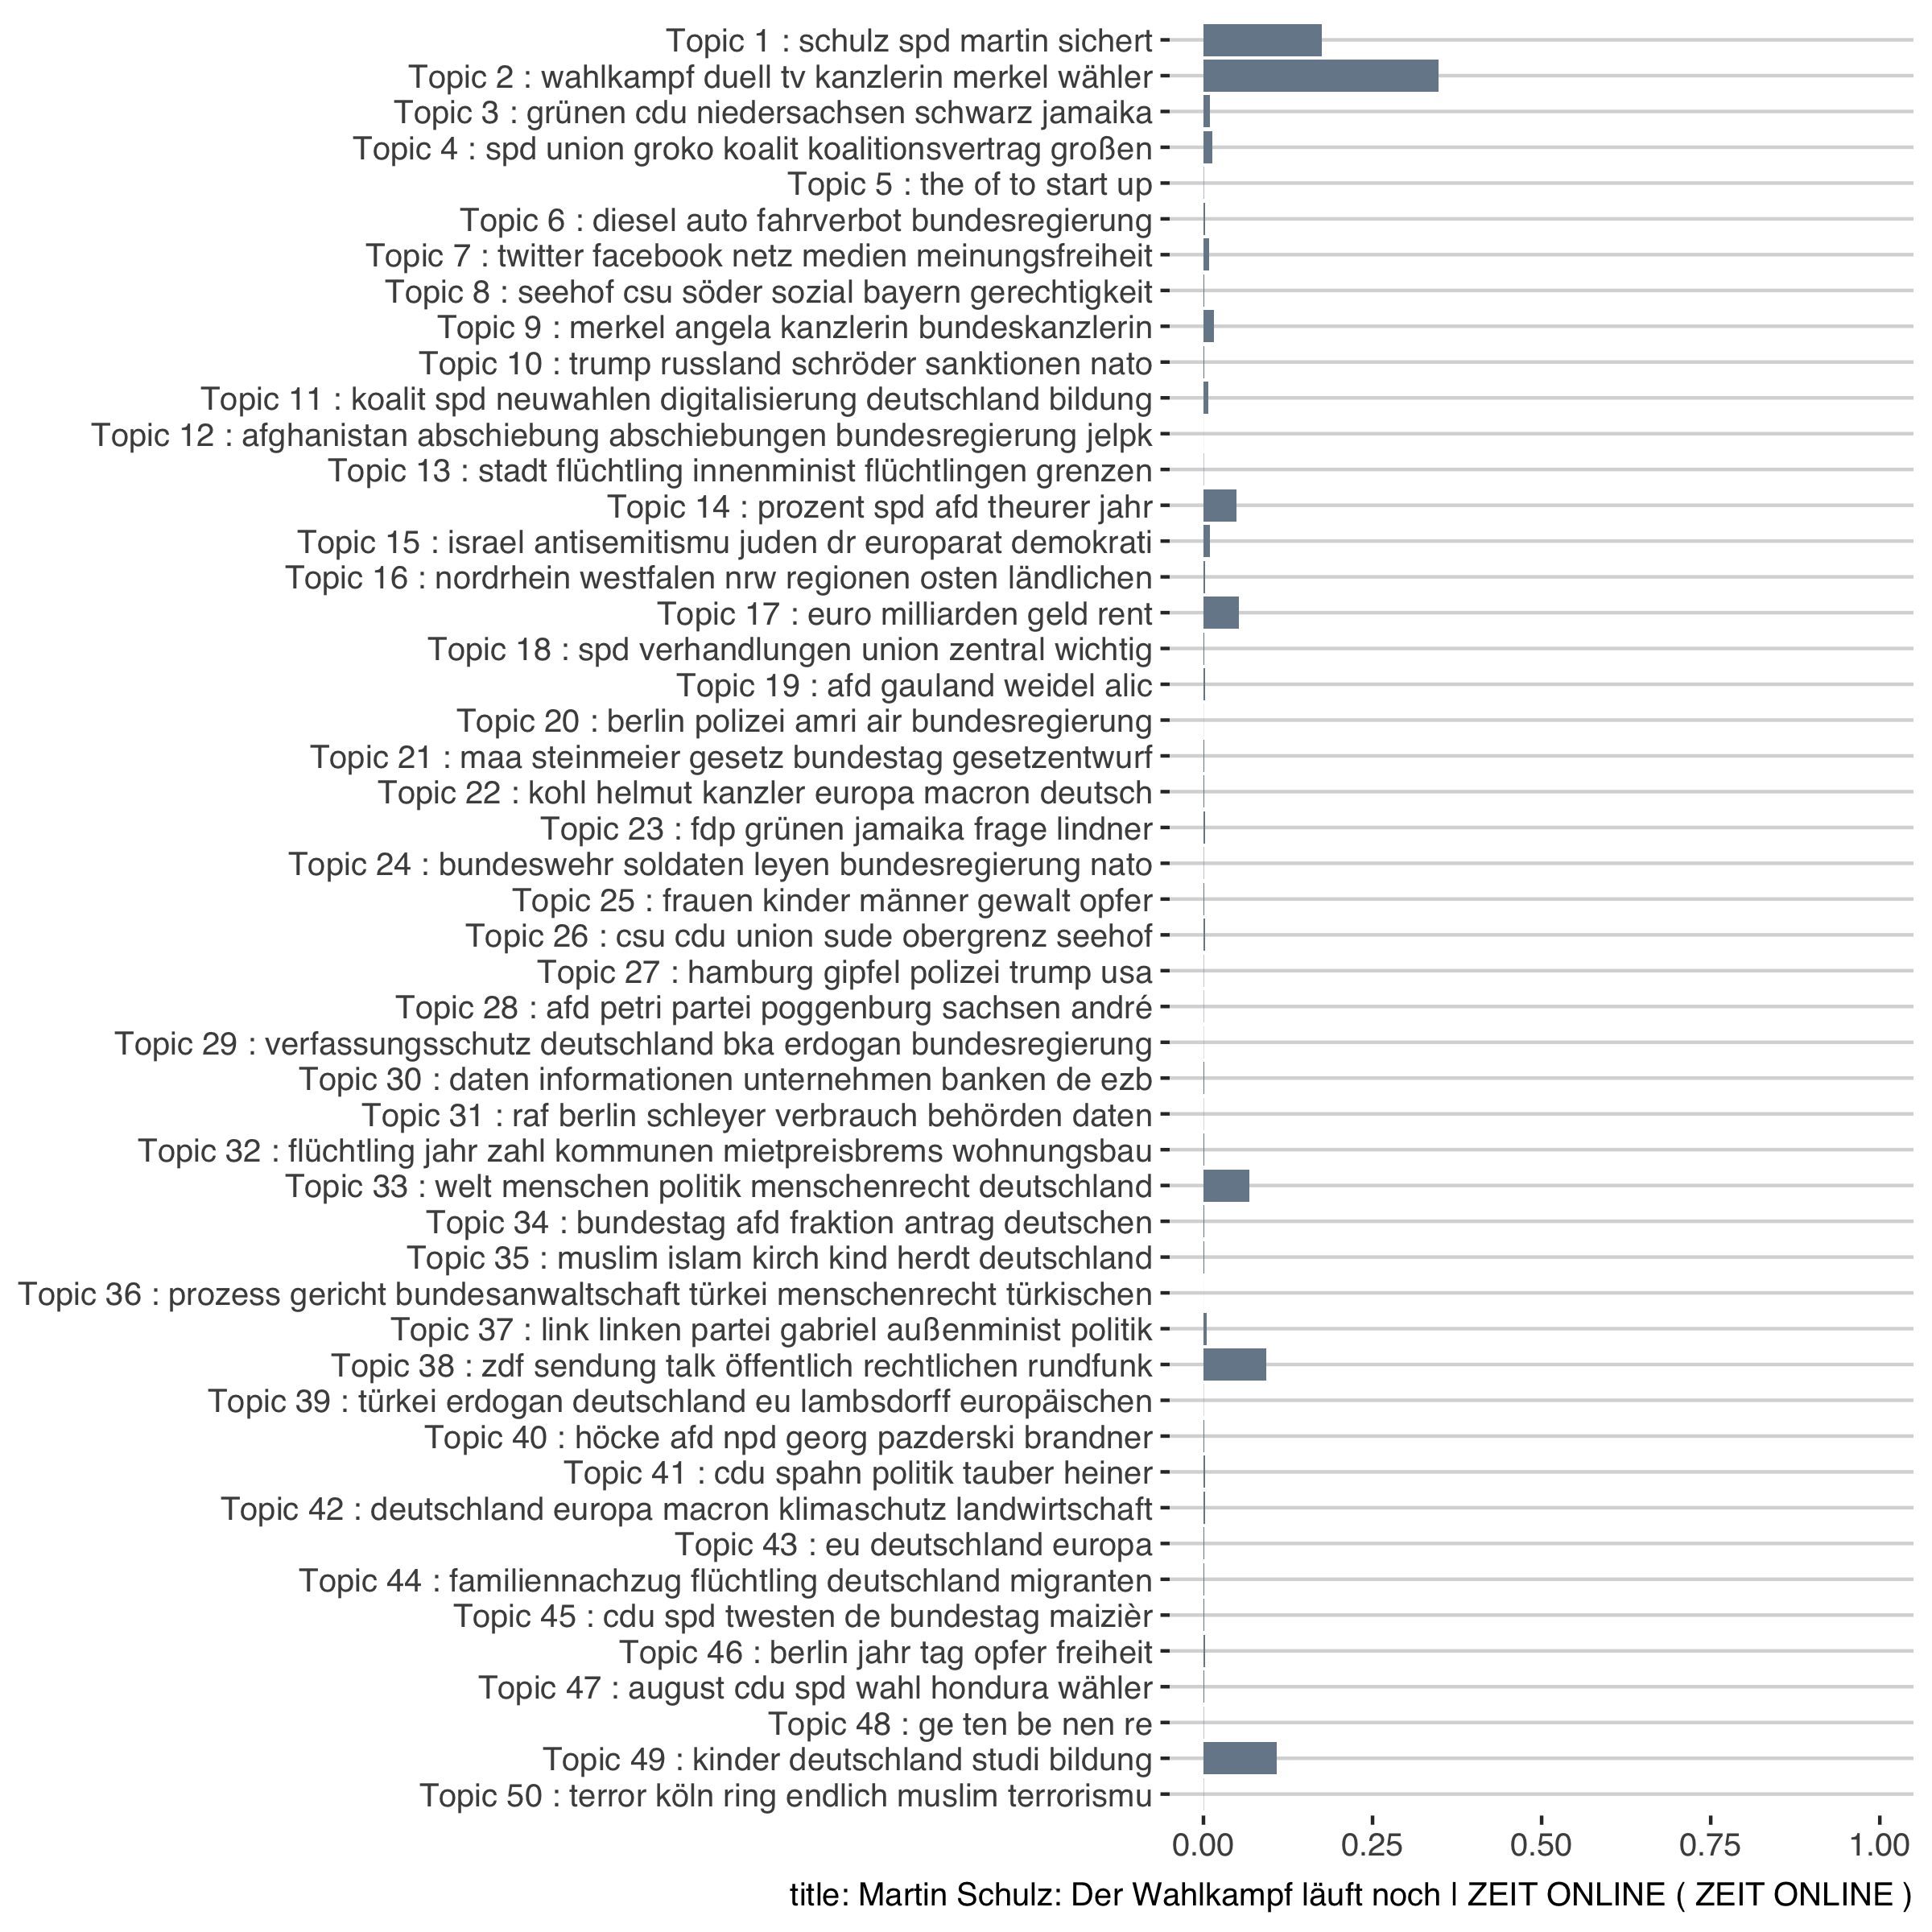
\includegraphics[width=0.6\textwidth]{../figs/doc_topic_distr}
	\label{fig_doc_topic_distr}
	\end{center}
\end{figure}

The average of each topic across all documents results in the expected probability of a topic across the whole corpus. As shown in Figure \ref{fig_expected_freq},\footnote{Results a shown in Appendix \ref{a_proportion}} topic 23 - which apparently deals with the issue of the Jamaica Coalition - is the most common topic. Topic 4, which deals with the coalition negotiations of the grand coalition ("GroKo") follows closely behind. 
%
%\begin{figure}[H]
%\begin{center}
%	\caption{Document-Topic distribution (example document) }
%	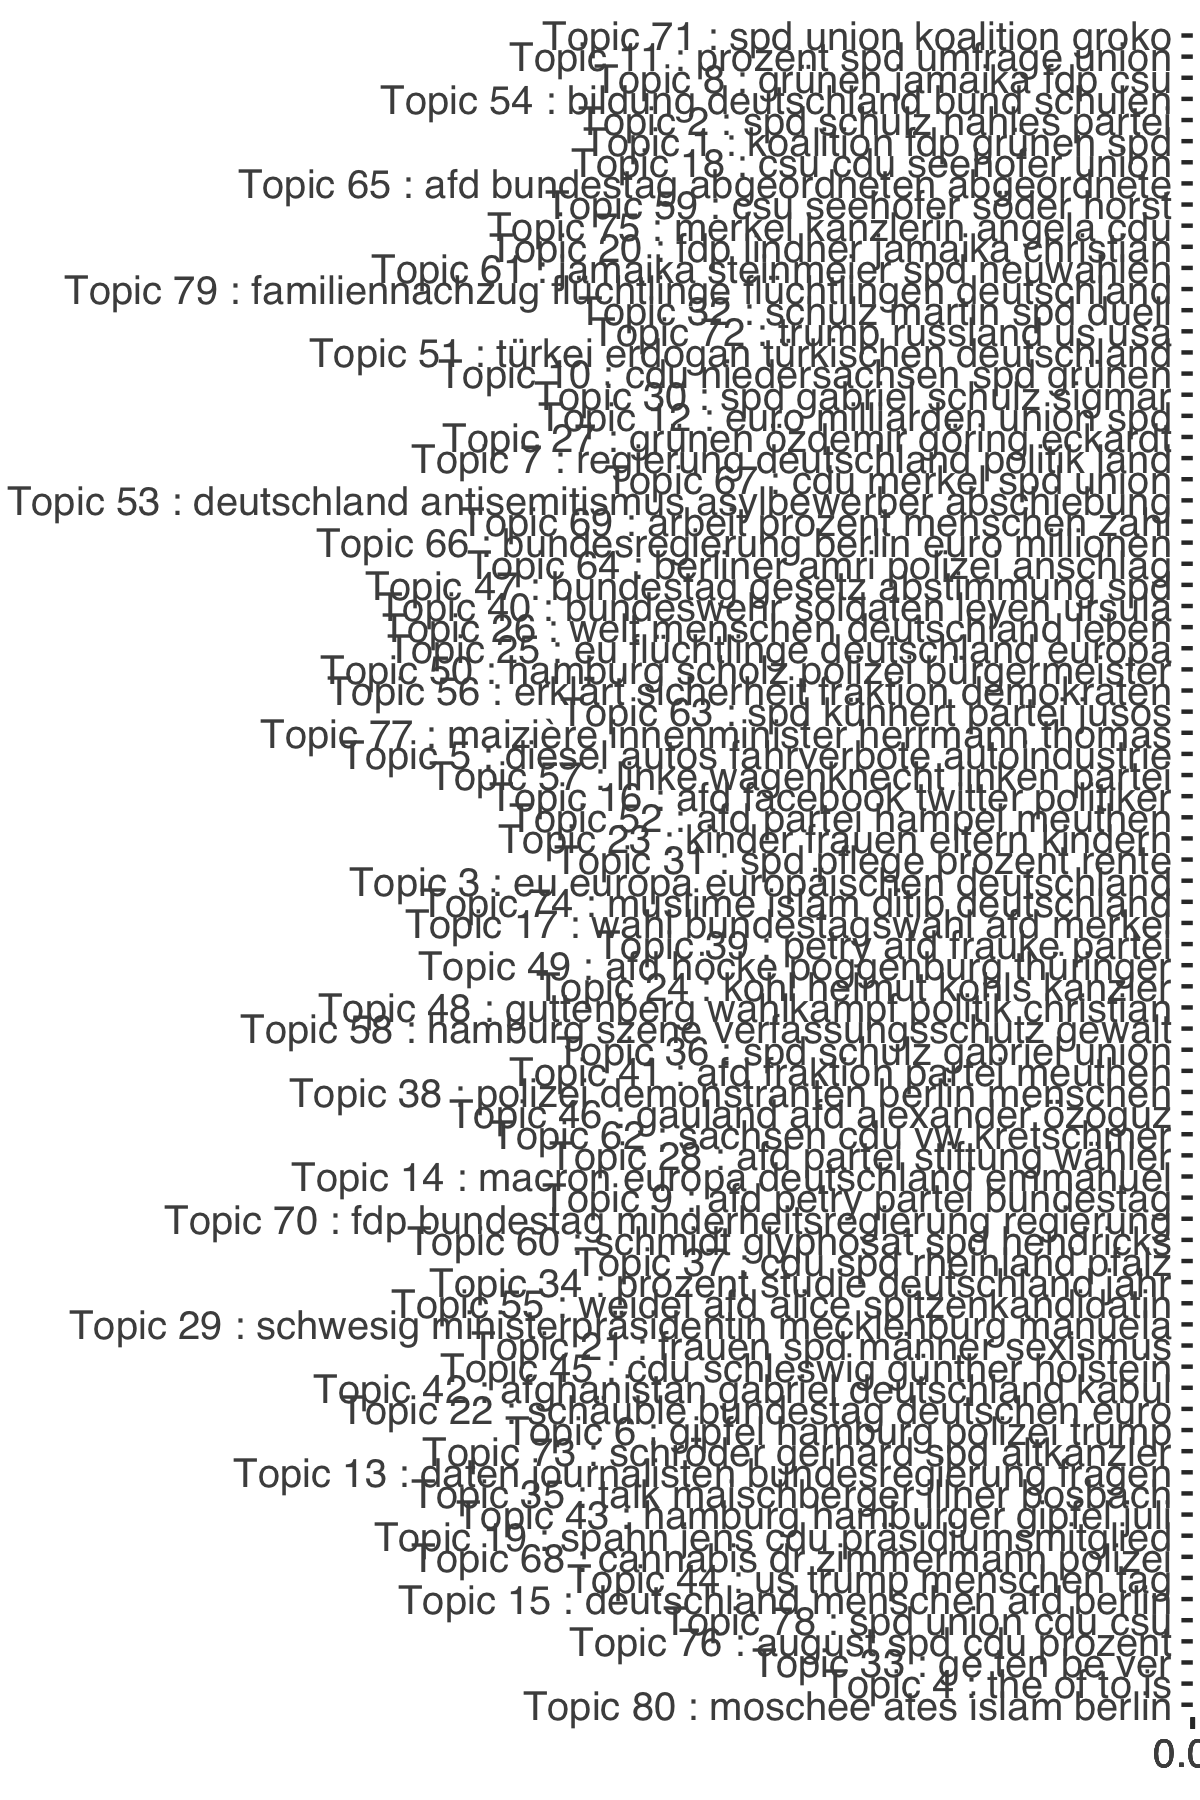
\includegraphics[width=0.8\textwidth]{../figs/topic_proportion}
%	\label{fig_expected_freq}
%	\end{center}
%\end{figure}

%------------------------------
%----- Topic proportion by type
%------------------------------

To calculate the mean topic probability for each source, the documents the average value of all documents belonging to that source is calculated. 
For each source the average distribution of each topic is calculated. 

\begin{figure}[H]
	\begin{center}
	\caption{Topic probablity}
		\begin{subfigure}[normla]{0.49\textwidth}
			\caption{Press releases}
			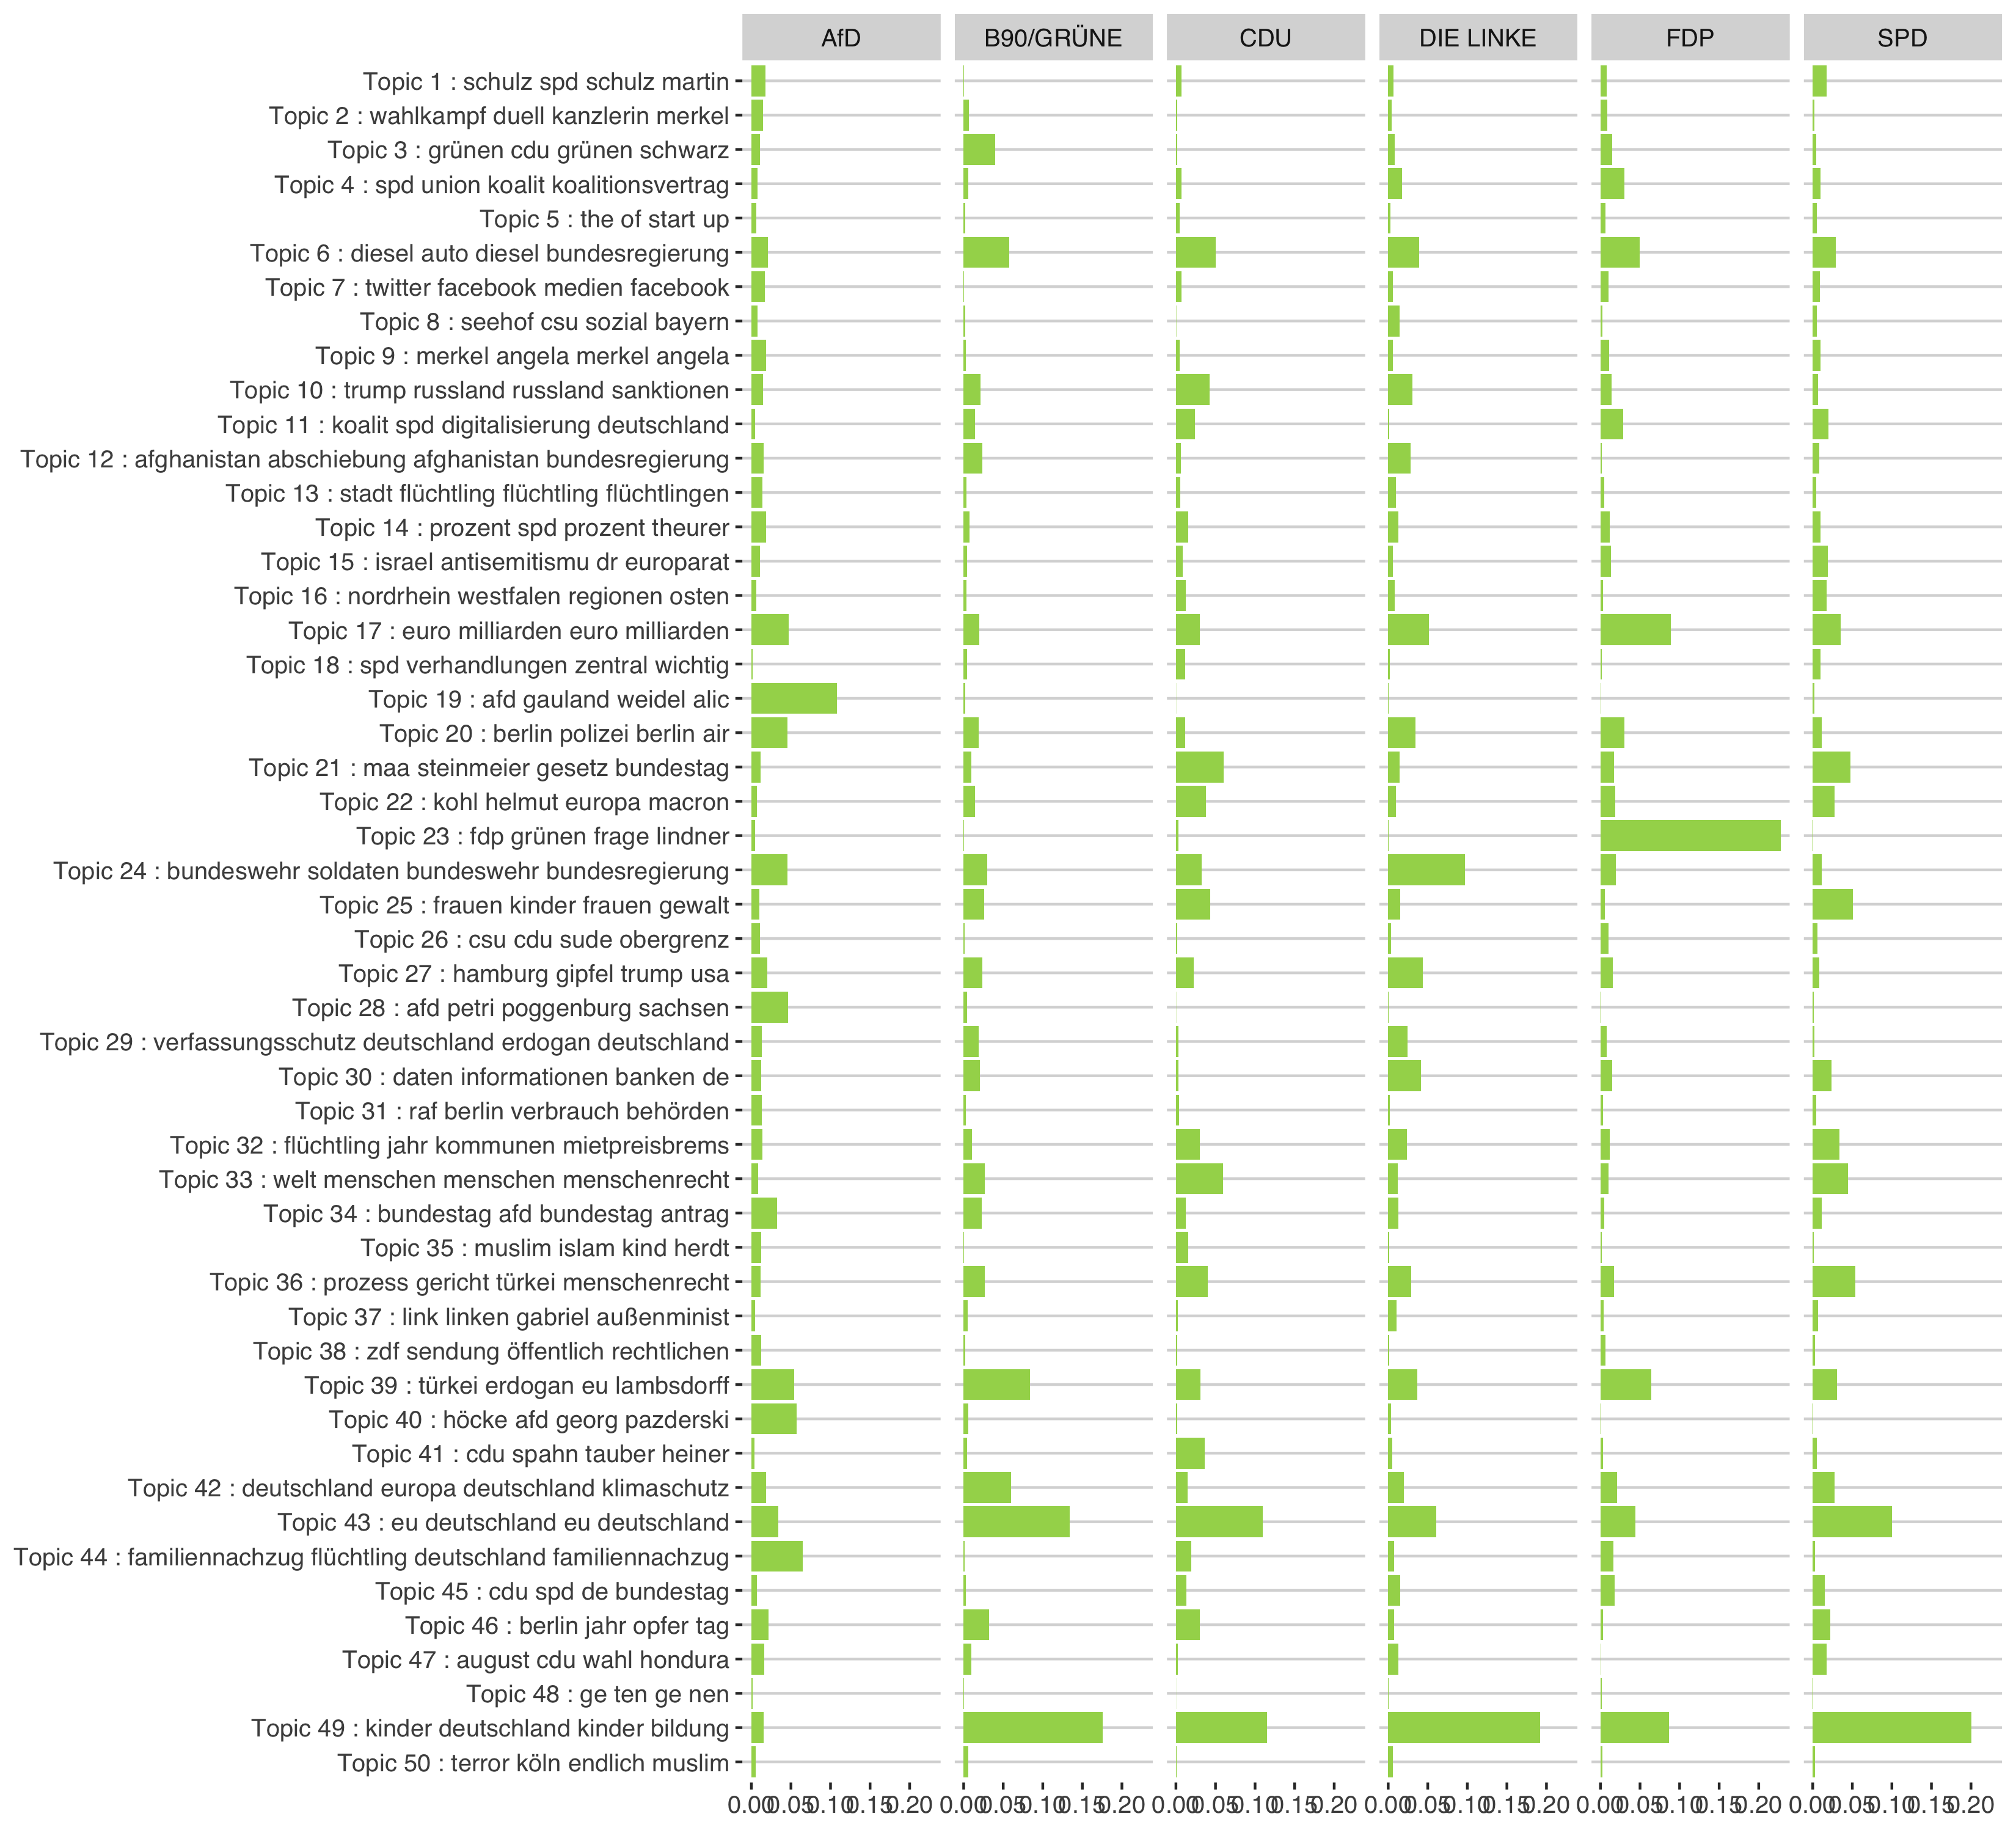
\includegraphics[width=\textwidth]{../figs/topic_proportion_press}
			\label{fig_tf_press}
		\end{subfigure}
		\begin{subfigure}[normla]{0.49\textwidth}
			\caption{News articles}
			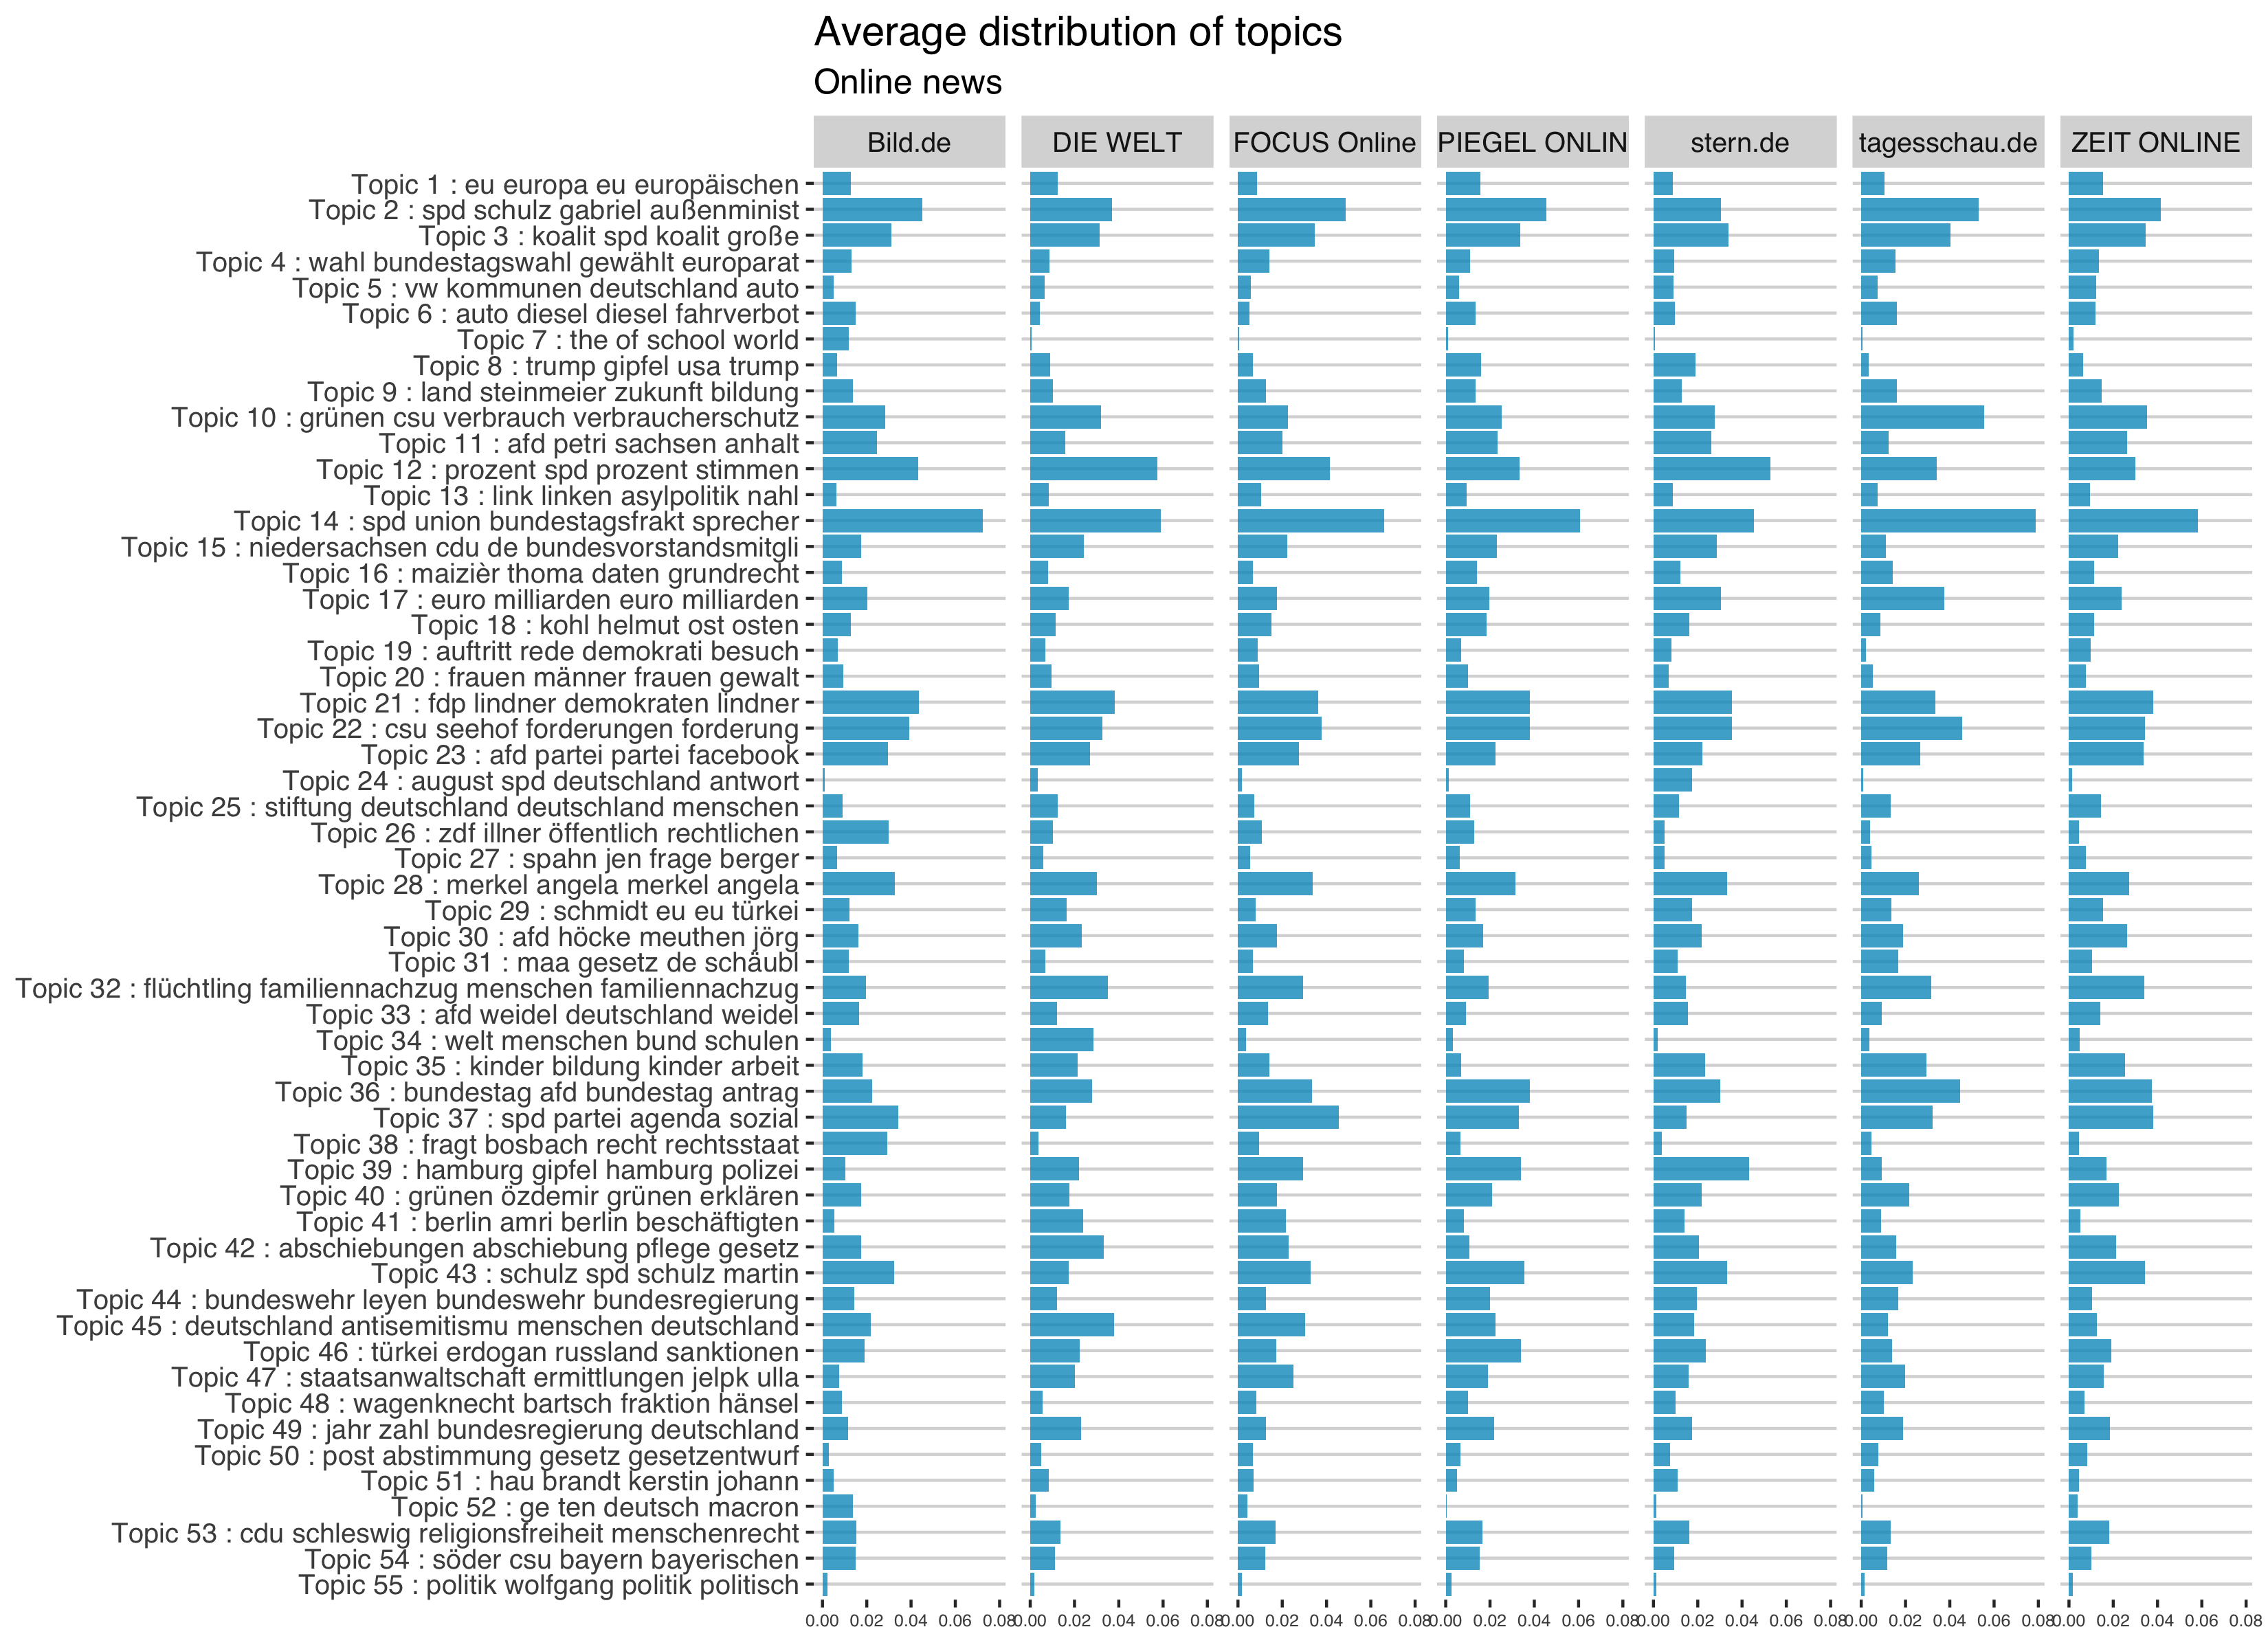
\includegraphics[width=\textwidth]{../figs/topic_proportion_news}
			\label{fig_tf_news}
		\end{subfigure}
	\end{center}
\end{figure}

% describe results !!!


\subsection{Weighted topic correlation}

First, the topic probability vector of each document is weighted by its sentiment value

\begin{figure}[H]
	\begin{center}
	\caption{Weighted topic probability}
		\begin{subfigure}[normla]{0.49\textwidth}
			\caption{Press releases}
			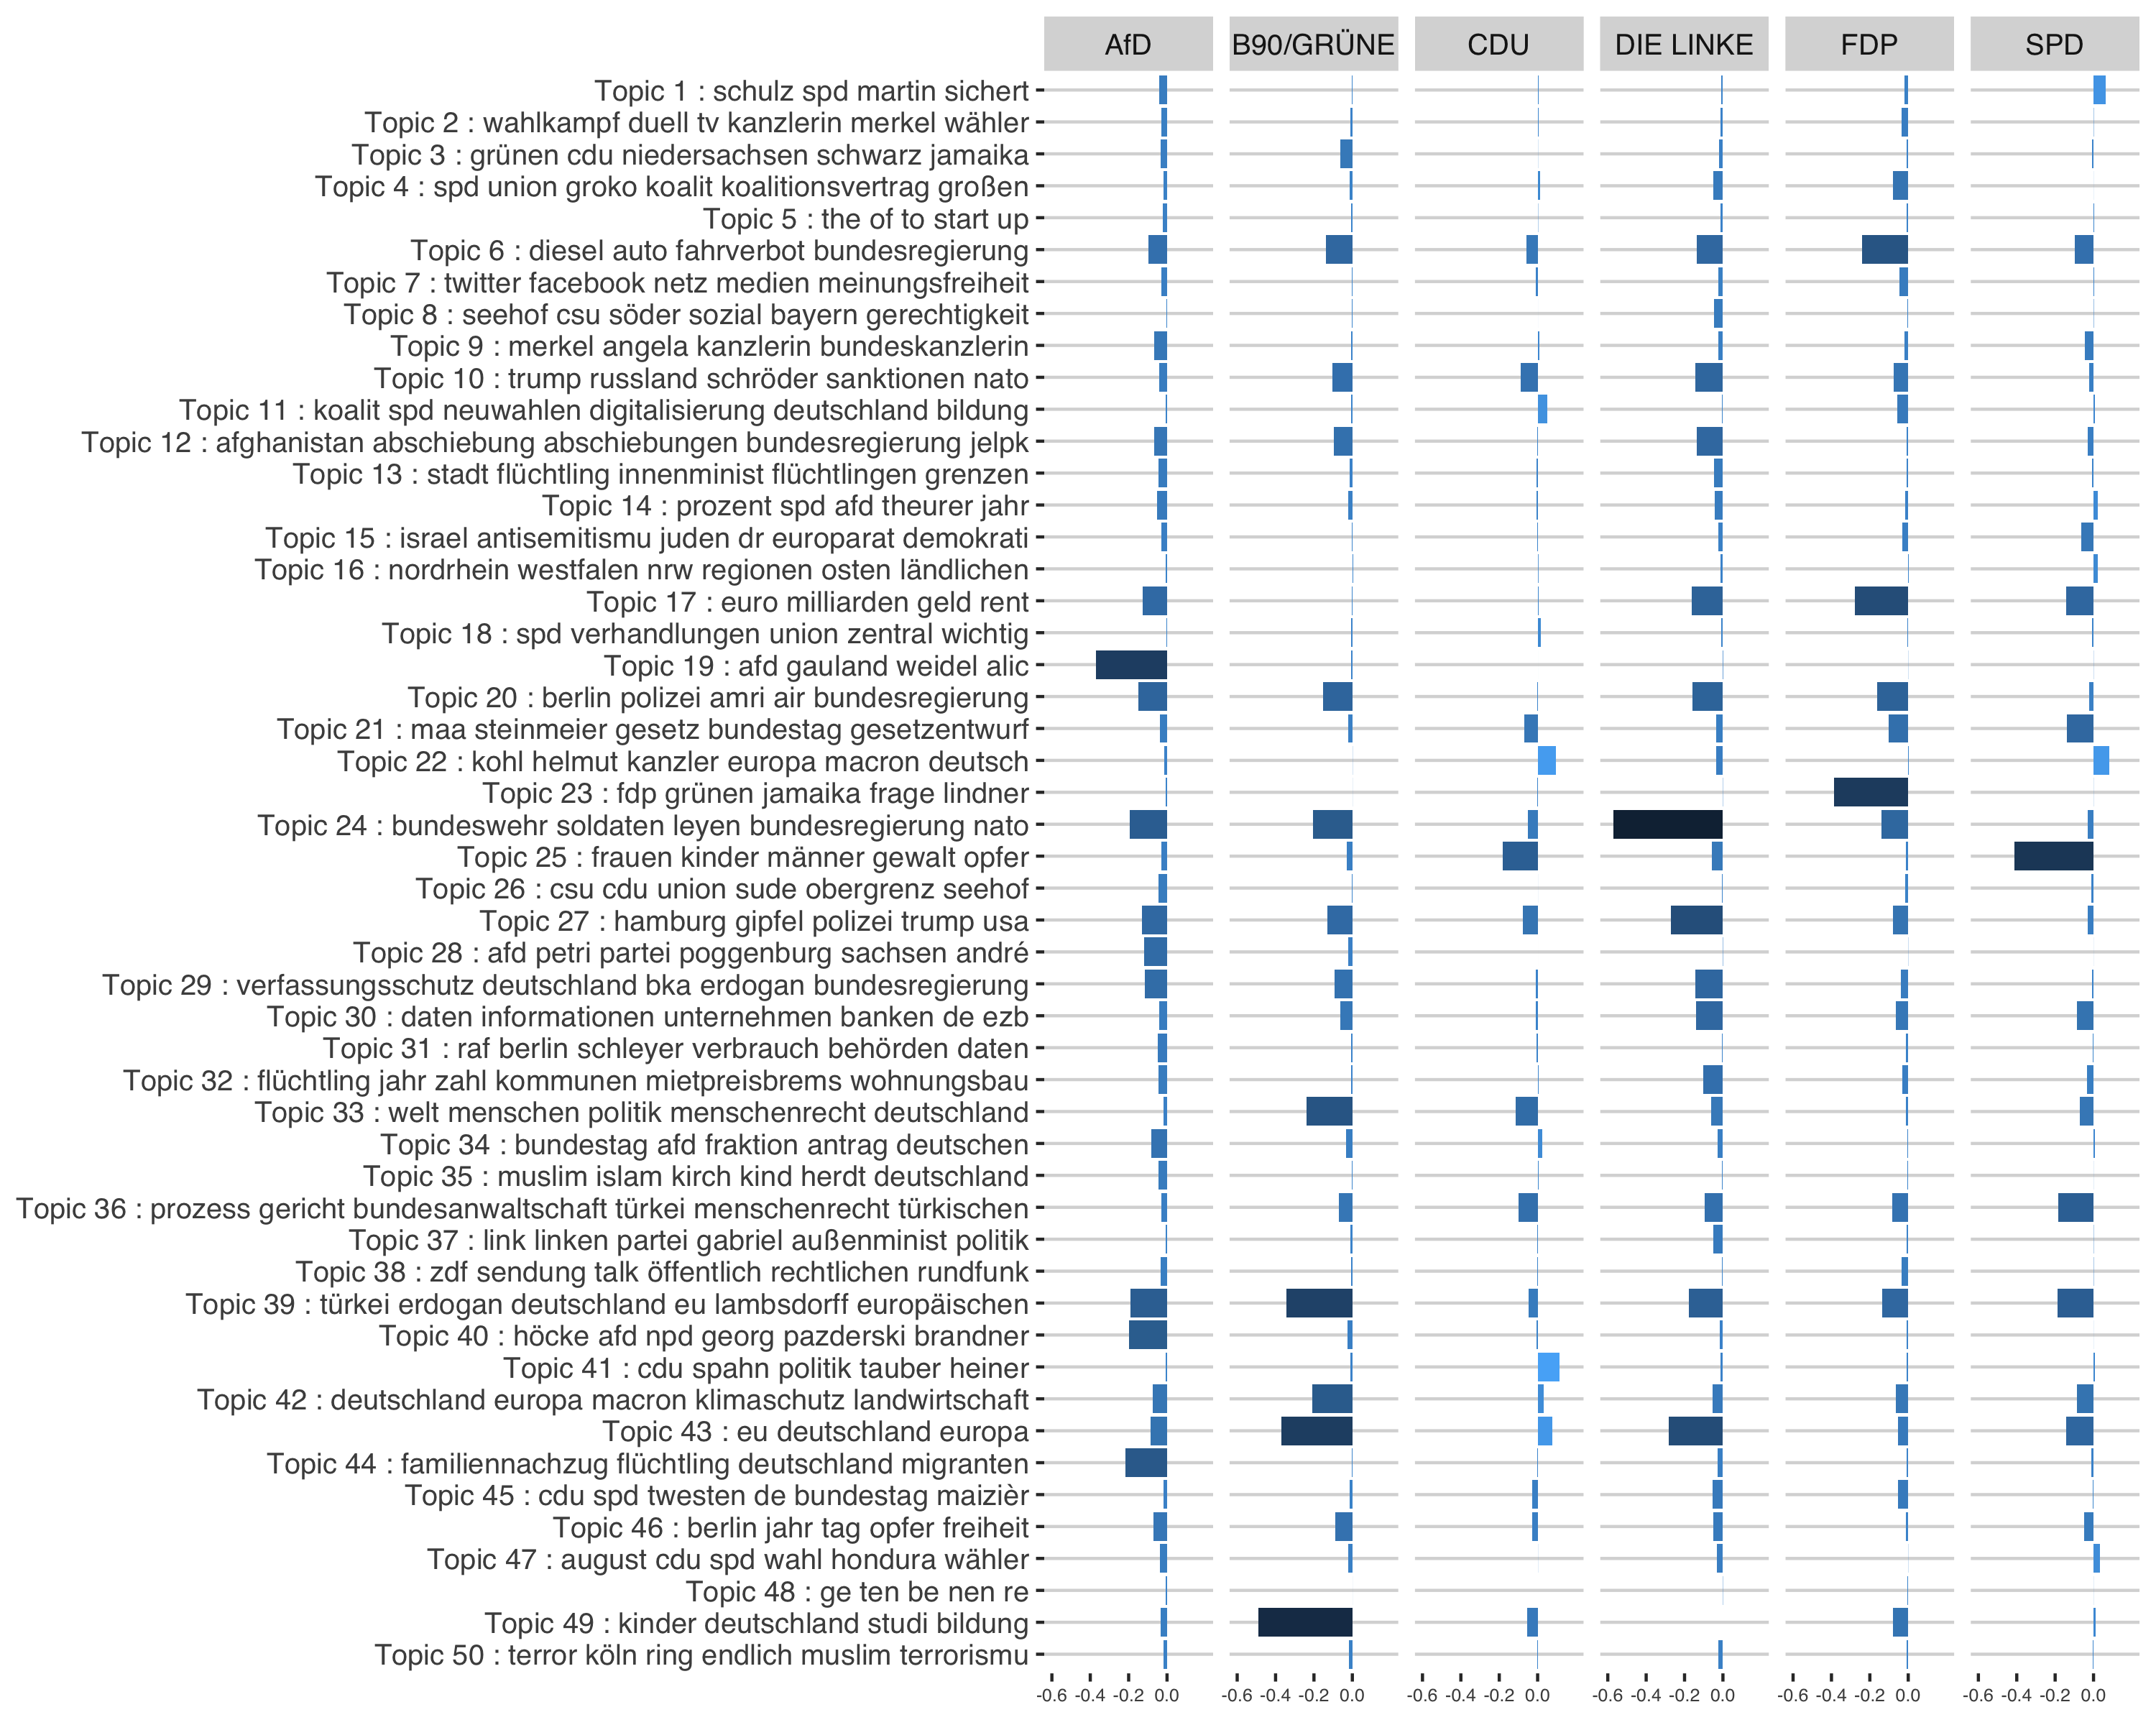
\includegraphics[width=\textwidth]{../figs/topic_sent_press}
			\label{fig_sent_press}
		\end{subfigure}
		\begin{subfigure}[normla]{0.49\textwidth}
			\caption{News articles}
			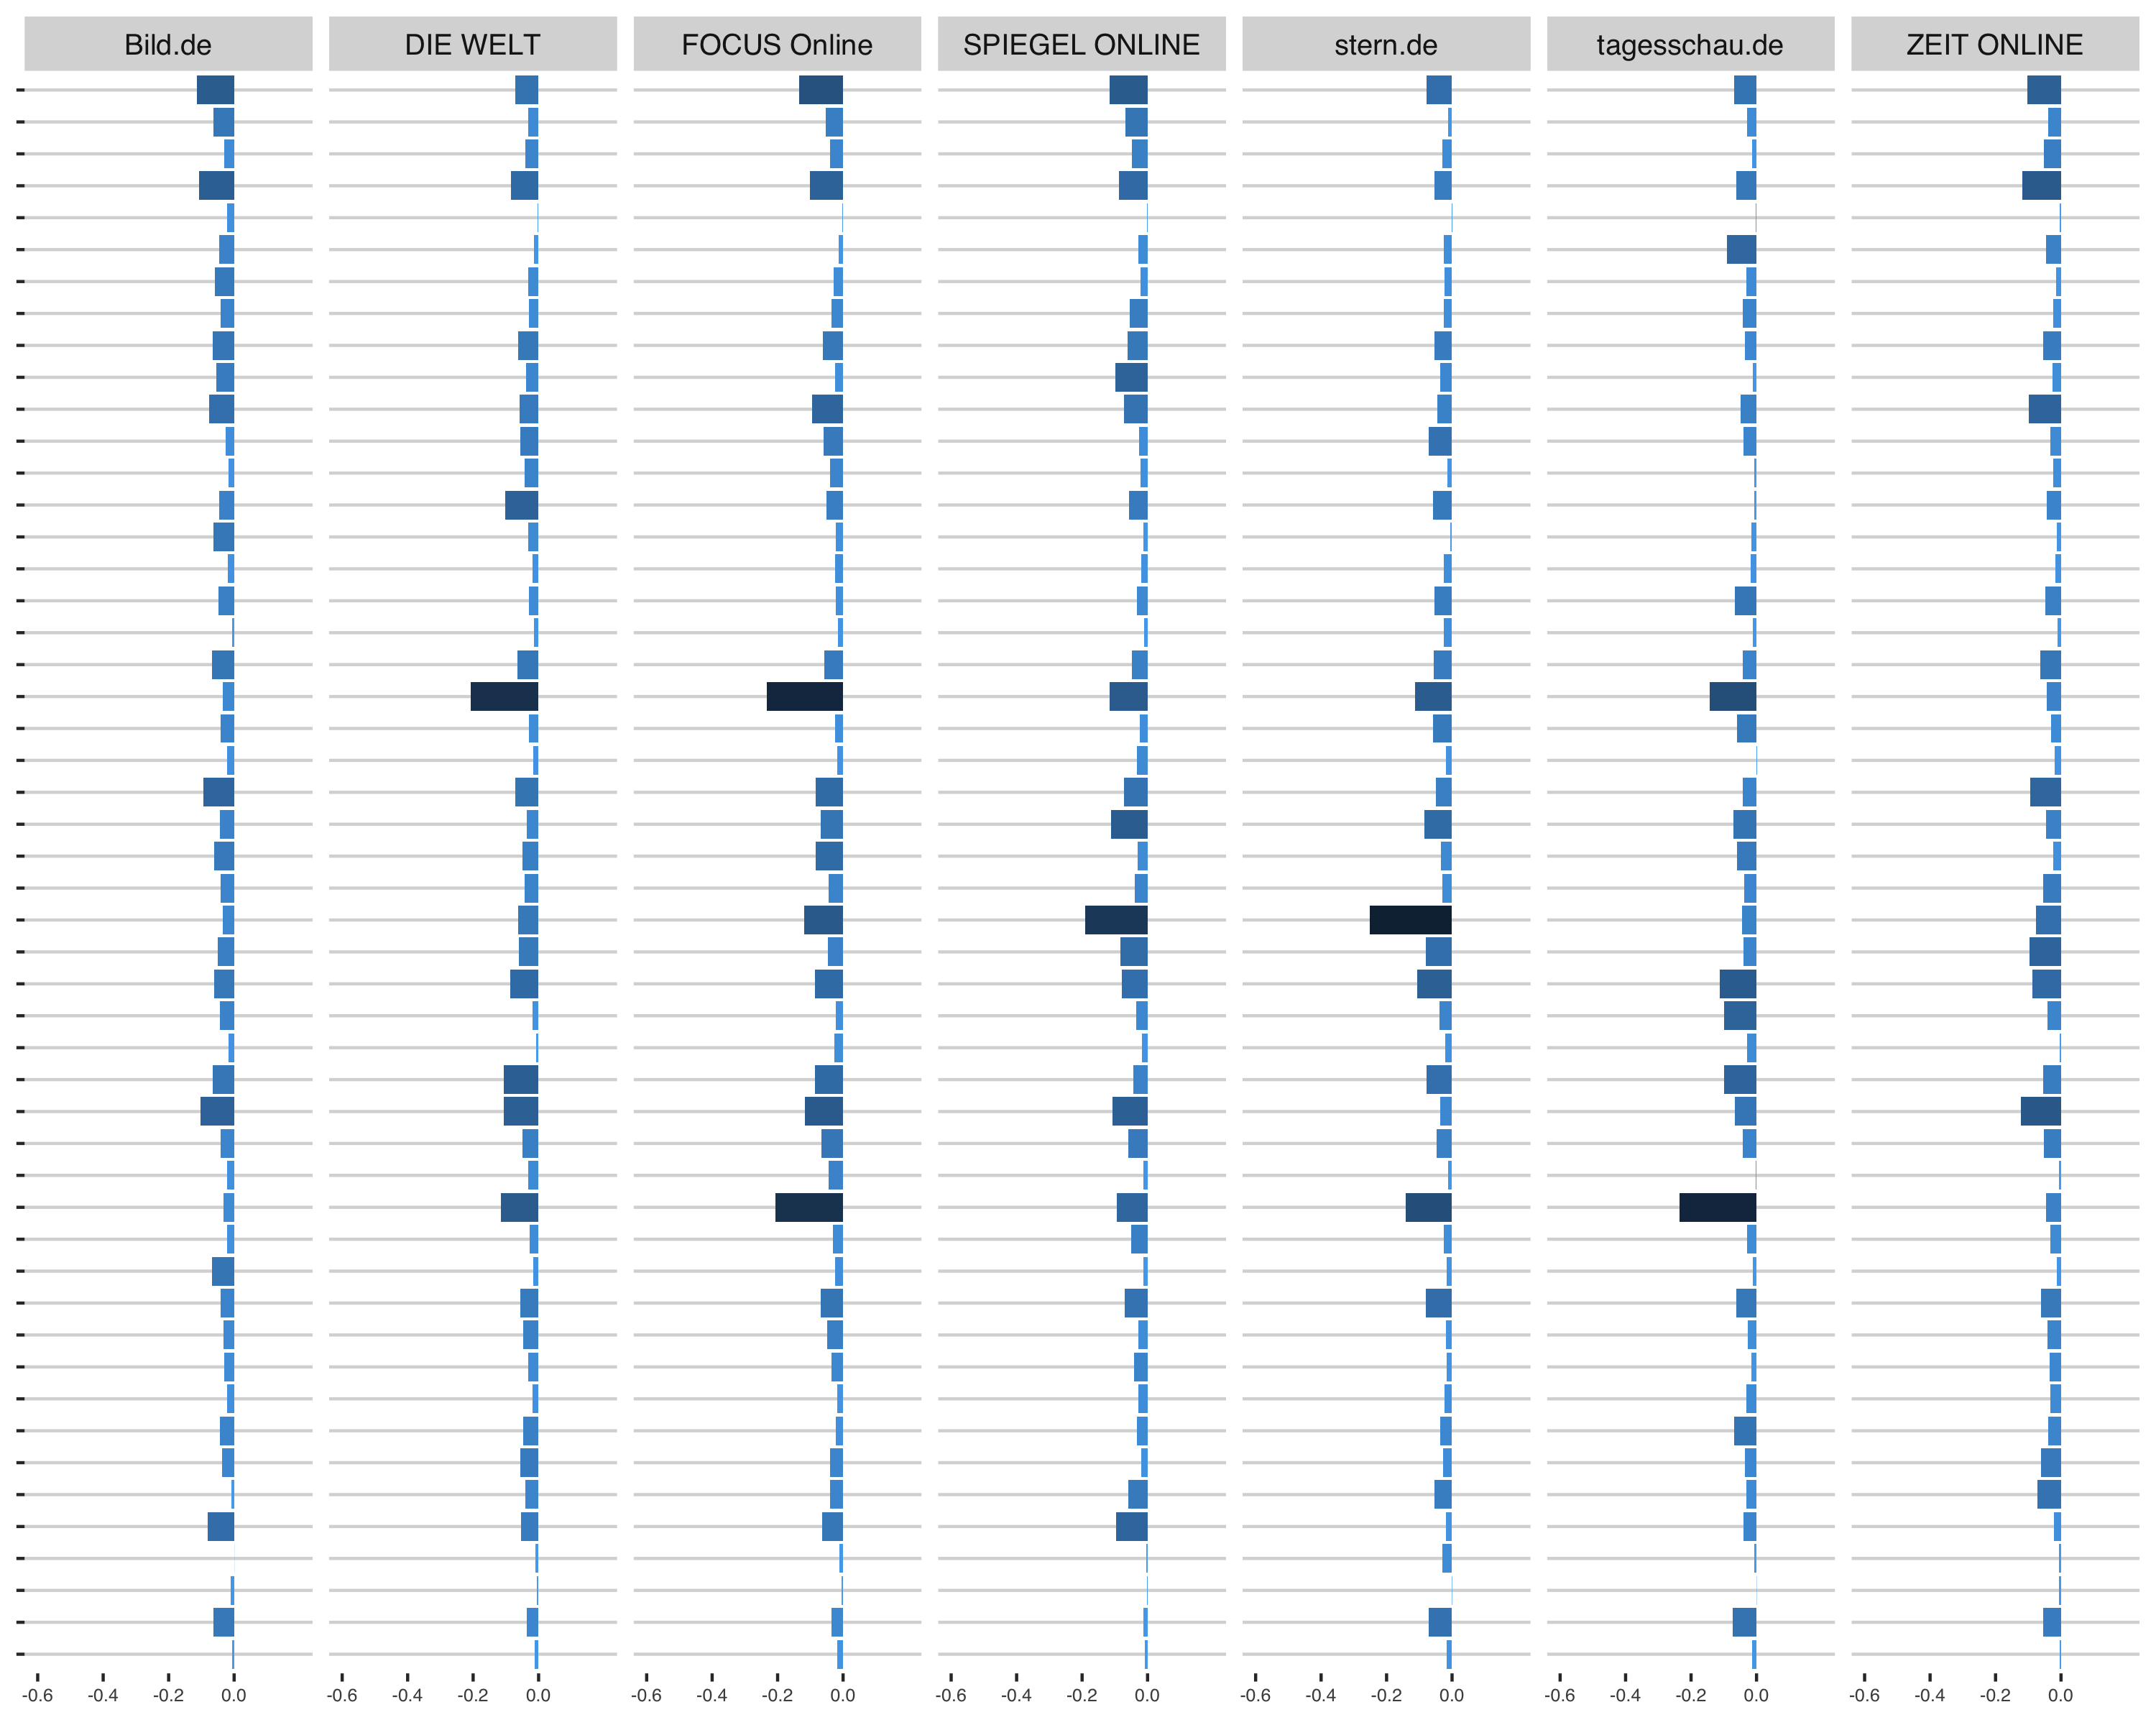
\includegraphics[width=\textwidth]{../figs/topic_sent_news}
			\label{fig_sent_news}
		\end{subfigure}
	\end{center}
\end{figure}

% describe results !!!

Subsequently, the bivariate correlations are estimated. 

\begin{figure}[H]
	\caption{Monthly topic correlation}
	\begin{center}
		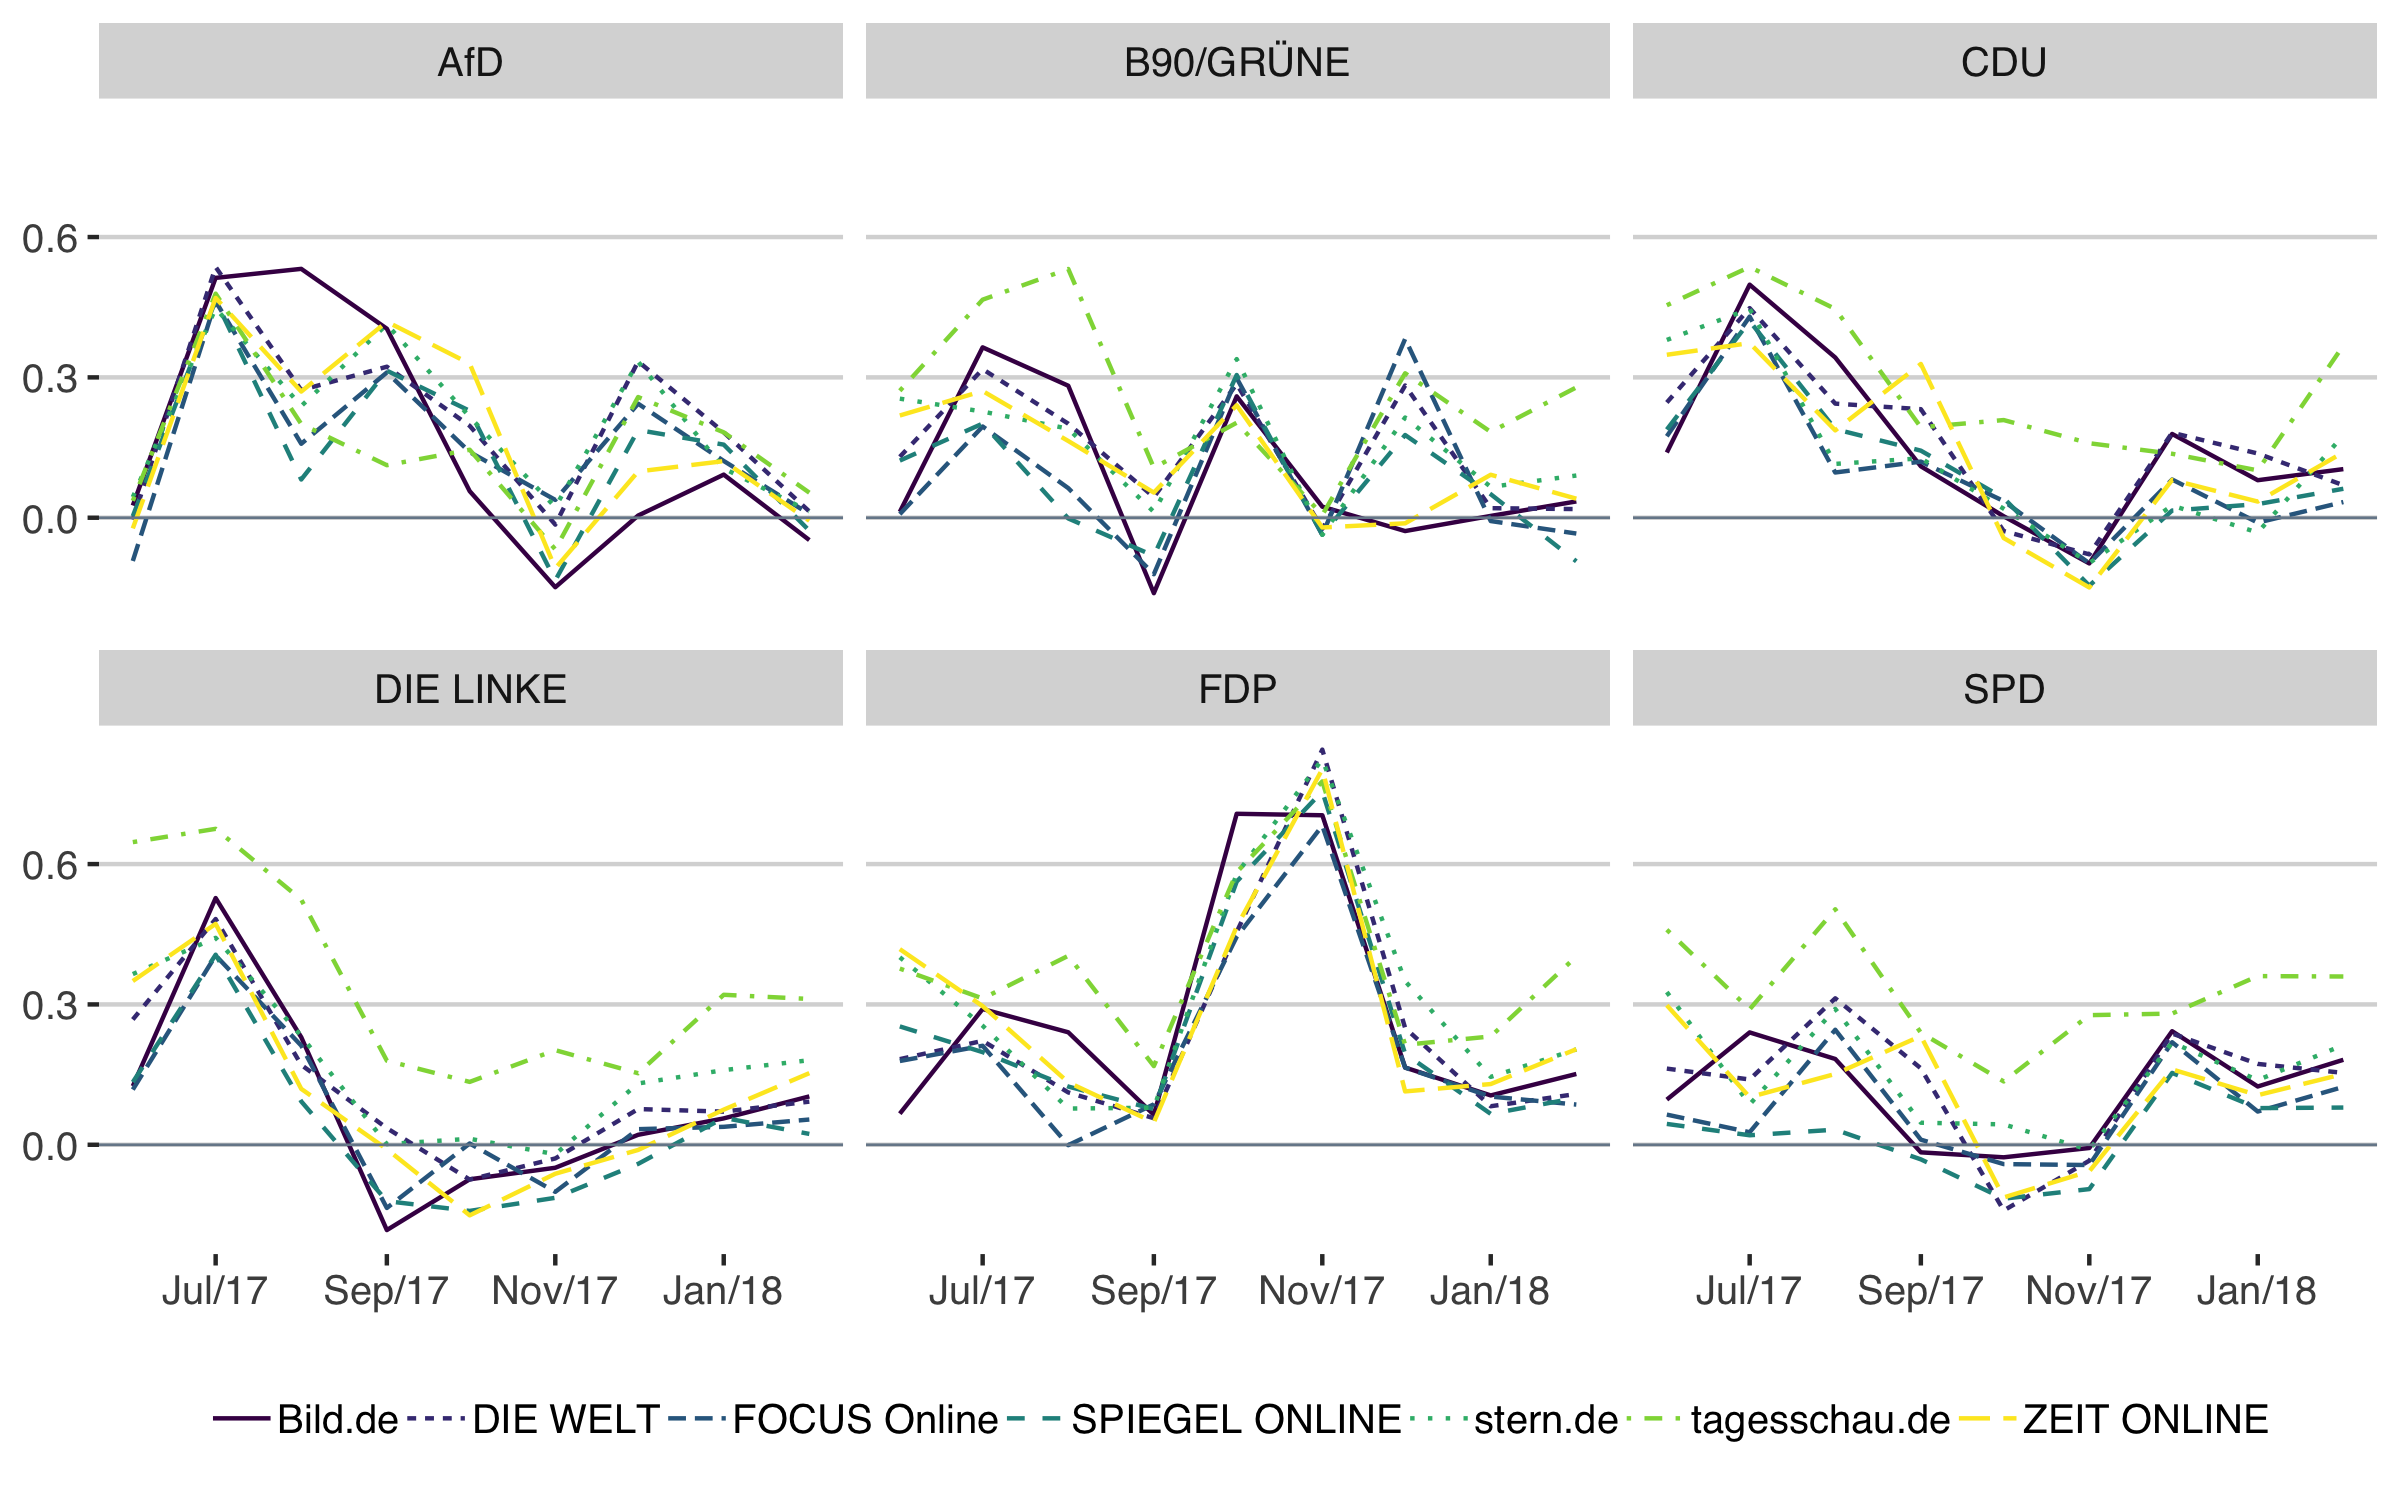
\includegraphics[width=0.7\textwidth]{../figs/corr_timeline}
	\end{center}
\end{figure}

\begin{figure}[H]
	\caption{Topic correlation}
	\begin{center}
		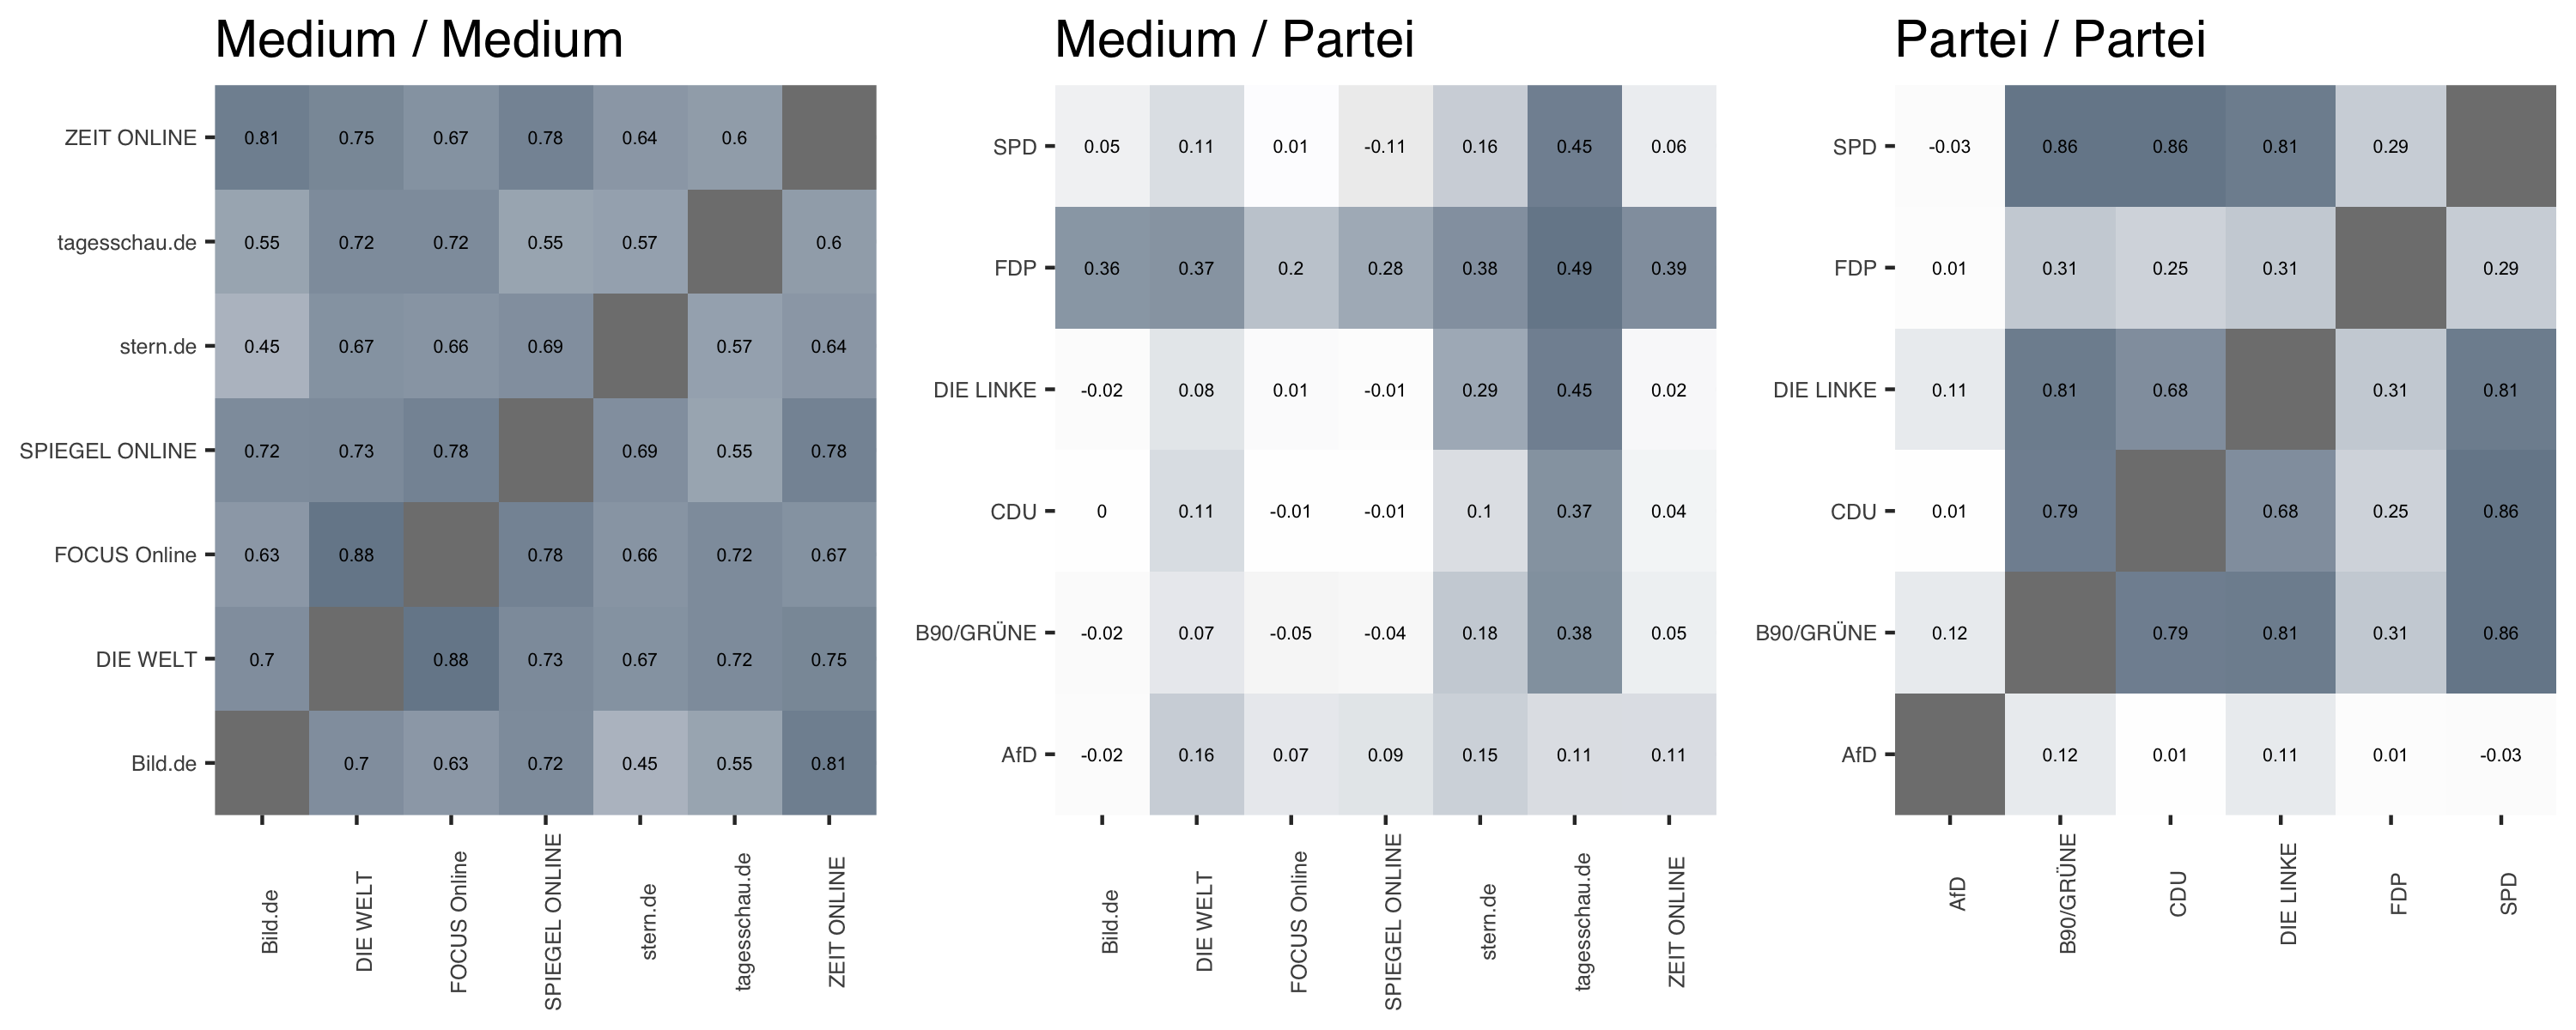
\includegraphics[width=\textwidth]{../figs/corrplot}
	\end{center}
\end{figure}

% describe results !!!

Obviously, due to their political or social relevance, not all potential topics receive the same amount of attention in the media. However, these factors should influence all media outlets equally. To calculate the relative topic correlation, I estimate the deviation of the topic correlation of a party in one medium from the average topic correlation of that party over all news paper.

\begin{figure}[H]
	\caption{Topic correlation - Radarcharts}
	\begin{center}
		\begin{subfigure}[normla]{0.42\textwidth}
			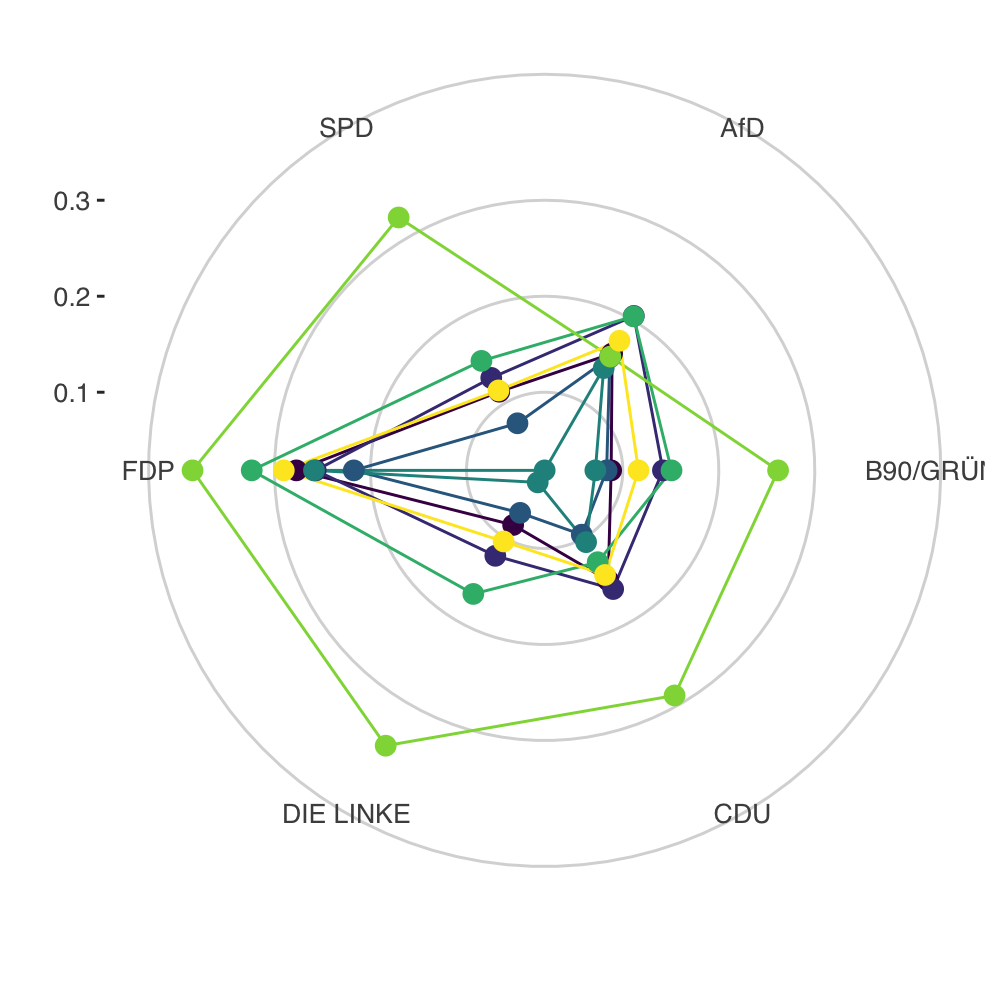
\includegraphics[width=\textwidth]{../figs/radar_corr}
			\caption{absolute values}
		\end{subfigure}
		\begin{subfigure}[normla]{0.52\textwidth}
			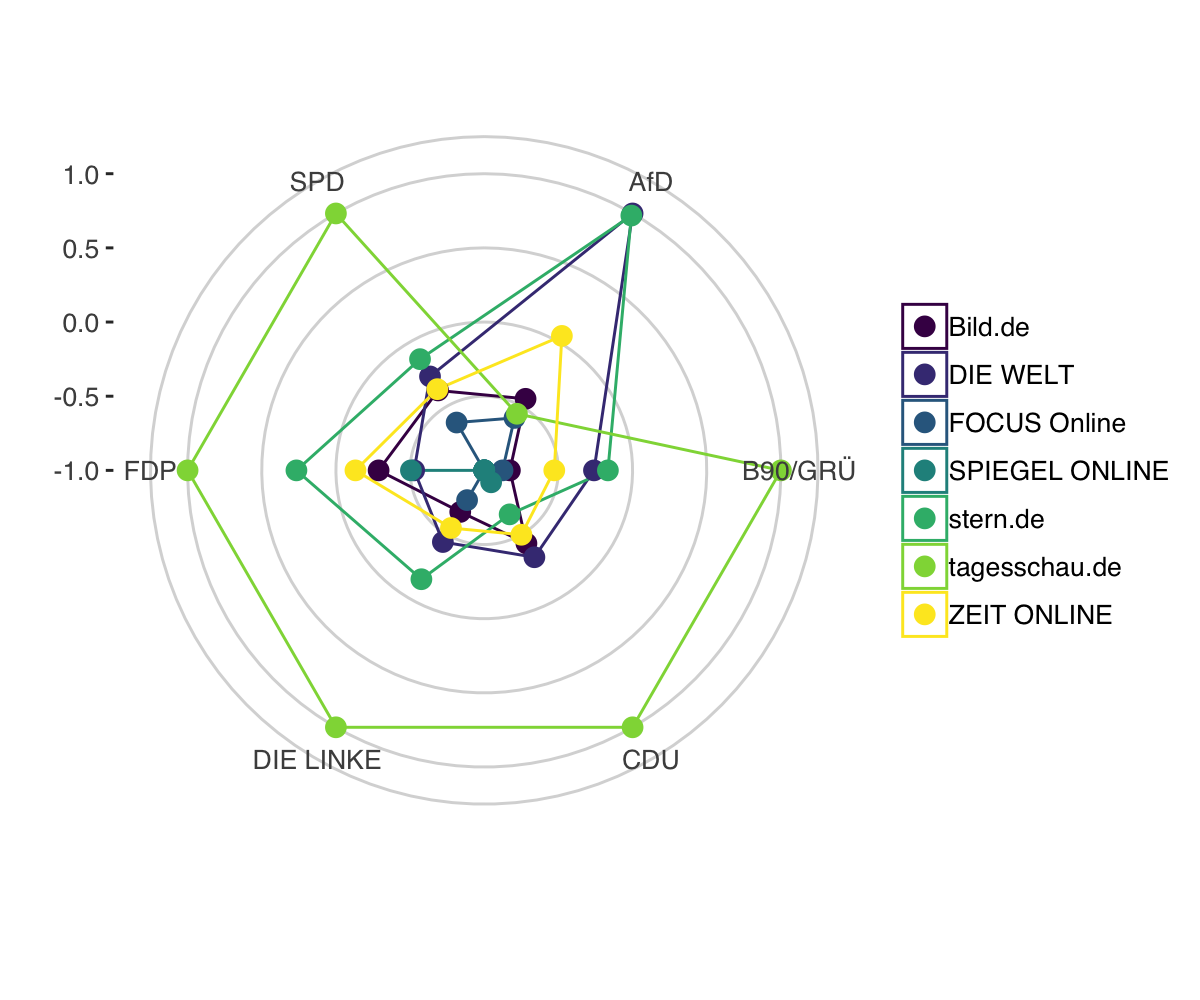
\includegraphics[width=\textwidth]{../figs/radar_corr_rescaled}
			\caption{relative values}
		\end{subfigure}
	\end{center}
\end{figure}

\subsection{Reader Preferences}\label{ch_readerpref}

\section{Conclusion}

The ongoing discussion about the influence of digital media on the political opinion-forming process addresses the question whether there are convergence tendencies within the mass media and whether the reporting in the media correlates with the voting preferences. To analyze this question, this paper examines .... 

Using text data of 14,937 online news articles from seven German news providers about domestic politics, I first estimate a Structural Topic Model to find the latent topics in the news articles ...

\pagebreak

\printbibliography

\appendix
\section{Appendices}

\subsection{Visibility}\label{a_visibility}

% latex table generated in R 3.5.1 by xtable 1.8-3 package
% Sat Apr 20 11:16:53 2019
\begin{table}[ht]
\centering
\begin{tabular}{lrrrrrr}
  \hline
medium & AfD & FDP & Grüne & Linke & SPD & Union \\ 
  \hline
Bild.de & 0.23 & 0.27 & 0.32 & 0.18 & 0.53 & 0.65 \\ 
  DIE WELT & 0.25 & 0.25 & 0.33 & 0.21 & 0.50 & 0.62 \\ 
  FOCUS Online & 0.21 & 0.21 & 0.26 & 0.18 & 0.46 & 0.55 \\ 
  SPIEGEL ONLINE & 0.23 & 0.25 & 0.33 & 0.22 & 0.56 & 0.65 \\ 
  stern.de & 0.25 & 0.28 & 0.35 & 0.24 & 0.53 & 0.63 \\ 
  tagesschau.de & 0.15 & 0.18 & 0.28 & 0.14 & 0.37 & 0.45 \\ 
  ZEIT ONLINE & 0.27 & 0.28 & 0.38 & 0.25 & 0.60 & 0.73 \\ 
   \hline
\end{tabular}
\caption{Visibility} 
\end{table}


\subsection{Generative Process of STM}\label{a_generativeProcess}

 The following describes the generative process for filling the $n^{th}$ word-position in document $d$ in the case of the STM \citep{roberts_structural_2013}: As in the case of conventional models, first a specific topic $z_{dn}$ is assigned, according to the topic distribution for that document $\theta$ through the process:

\begin{equation}
	z_{dn}|\theta_d \sim \textrm{Multinomial}(\theta_d).
\end{equation}

To incorporate the covariate values for that document, a topic-prevalence vector $\theta_d$ is drawn from a logistic-normal distribution:

\begin{equation}
	\theta_d|y_{d\gamma},\Sigma \sim \textrm{LogisticNormal}(\mu = y_{d\gamma}\Sigma),
\end{equation}

where $y_d\gamma$ lists the values of the metadata covariates for document $d$ and $\gamma$ relates these covariate values to the topic-prevalence. 

Conditional in the topic chosen ($z_{dn}$), a specific word $w_{dn}$, is selected from the overall corpus vocabulary $V$, using the following process:

\begin{equation}
	w_{dn}|z_{dn},\phi_{dkv} \sim \textrm{Multinomial}(\phi_{dk1},...,\phi_{dkV}),
\end{equation}

where the word probability $\phi_{dkv}$ is parameterized in terms of log-transformed rate deviations from the rates of a corpus-wide background distribution $m_v$ \citep{roberts_structural_2013}. The log-transformed rate deviations can then be specified by a collection of parameters $\lbrace \boldsymbol{\kappa} \rbrace$, where $\kappa^{(t)}$ is a $K$-by-$V$ matrix containing the log-transformed rate deviations for each topic $k$ and term $v$, over the baseline log-transformed rate for term $v$. This matrix is the same for all $A$ levels of covariates. To put it differently, $\kappa^{(t)}$ indicates the importance of the term $v$ given topic $k$ regardless of the covariates. Similarly, $\kappa^{(c)}$ is a $A$-by-$V$ matrix, indicating the importance of the term $v$ given the covariate level $c$ regardless of the topic. Finally, $\kappa^{(i)}$ is a $A$-by-$K$-by-$V$ matrix, collecting the covariate-topic effects:

\begin{equation}
	\phi_{dkv}|z_{dn}=\frac{\textrm{exp}(m_v+\kappa^{(t)}_{kv},\kappa^{(c)}_{y_dv}+\kappa^{(i)}_{y_dkv})}{\sum_v \textrm{exp}(m_v+\kappa^{(t)}_{kv},\kappa^{(c)}_{y_dv}+\kappa^{(i)}_{y_dkv})}.
\end{equation}

The STM maximizes the posterior likelihood that the observed data were generated by the above data-generating process using an iterative approximation-based variational expectation-maximization algorithm\footnote{A technical description of this maximization process can be found in \citet{roberts_model_2016}} available in R's stm package \citep{roberts_stm:_2016}. 

\subsection{Most frequent words}\label{a_labels}

% latex table generated in R 3.6.0 by xtable 1.8-4 package
% Mon Jun  3 15:21:32 2019
\begin{table}[ht]
\centering
\begin{tabular}{lll}
  \hline
Topic & News articles & Press releases \\ 
  \hline
1 & schulz spd martin gabriel partei & schulz martin sichert wahlkampf kanzlerkandidat \\ 
  2 & wahlkampf duell tv lang spricht & kanzlerin merkel wähler lang tv \\ 
  3 & grünen cdu niedersachsen grüne fdp & grünen schwarz jamaika rot gelb \\ 
  4 & spd union groko koalit koalitionsverhandlungen & koalit koalitionsvertrag großen große groko \\ 
  5 & the of to on it & start up the german it \\ 
  6 & diesel auto fahrverbot autoindustri deutschen & diesel bundesregierung auto fahrverbot vw \\ 
  7 & twitter facebook netz tweet medien & medien facebook meinungsfreiheit internet netzwerkdurchsetzungsgesetz \\ 
  8 & seehof csu söder bayern horst & sozial bayern gerechtigkeit partei sahra \\ 
  9 & merkel angela kanzlerin cdu bundeskanzlerin & merkel angela bundeskanzlerin deutschland neuwahlen \\ 
  10 & trump russland schröder usa putin & russland sanktionen nato krim deutschland \\ 
  11 & koalit spd neuwahlen jamaika große & digitalisierung deutschland bildung digital zukunft \\ 
  12 & afghanistan abschiebung abschiebungen abgeschoben deutschland & afghanistan bundesregierung jelpk ulla abschiebungen \\ 
  13 & stadt flüchtling innenminist herrmann flüchtlingen & flüchtling flüchtlingen grenzen menschen migranten \\ 
  14 & prozent spd afd bundestagswahl umfrag & prozent theurer jahr zahl zahlen \\ 
  15 & israel antisemitismu juden deutschland israelisch & dr europarat demokrati strack zimmermann \\ 
  16 & nordrhein westfalen nrw sachsen schwesig & regionen osten ländlichen ost ostdeutschland \\ 
  17 & euro milliarden geld millionen jahr & euro milliarden rent geld investitionen \\ 
  18 & spd verhandlungen union einigung cdu & zentral wichtig verhandlungen verbraucherschutz migrat \\ 
  19 & afd gauland weidel partei alexand & weidel alic gauland alexand deutschen \\ 
  20 & berlin polizei amri anschlag polizisten & berlin air bundesregierung polizei anschlag \\ 
  21 & maa steinmeier gesetz heiko bundespräsid & gesetz bundestag gesetzentwurf maa regelungen \\ 
  22 & kohl helmut kanzler einheit altkanzl & europa macron deutsch deutschland deutschen \\ 
  23 & fdp grünen jamaika lindner grüne & frage lindner grünen kubicki jamaika \\ 
  24 & bundeswehr soldaten leyen nato einsatz & bundeswehr bundesregierung nato syrien soldaten \\ 
  25 & frauen kinder männer jahr sexuel & frauen gewalt opfer mädchen deutschland \\ 
  26 & csu cdu union seehof obergrenz & sude obergrenz seehof forderung begrenzung \\ 
  27 & hamburg gipfel polizei demonstranten scholz & trump usa gipfel hamburg donald \\ 
  28 & afd petri partei frauk fraktion & poggenburg sachsen andré anhalt hampel \\ 
  29 & verfassungsschutz deutschland bka maizièr sicherheitsbehörden & erdogan deutschland bundesregierung türkischen verfassungsschutz \\ 
  30 & daten informationen unternehmen mitarbeit bundesregierung & banken de ezb konzern masi \\ 
  31 & raf berlin schleyer terroristen entführung & verbrauch behörden daten uw terroristen \\ 
  32 & flüchtling jahr zahl bamf deutschland & kommunen mietpreisbrems wohnungsbau mieten sozialen \\ 
  33 & welt menschen politik deutschland land & menschen menschenrecht deutschland engag religionsfreiheit \\ 
  34 & bundestag afd fraktion abgeordneten parlament & bundestag antrag deutschen parlament parlamentarisch \\ 
  35 & muslim islam kirch feiertag muslimischen & kind herdt deutschland christen waldemar \\ 
  36 & prozess gericht bundesanwaltschaft nsu staatsanwaltschaft & türkei menschenrecht türkischen freilassung yücel \\ 
  37 & link linken partei wagenknecht spd & gabriel außenminist politik sigmar kort \\ 
  38 & zdf sendung talk bosbach politik & öffentlich rechtlichen rundfunk ard medien \\ 
  39 & türkei erdogan deutschland türkischen türkisch & eu lambsdorff europäischen europäisch parlament \\ 
  40 & höcke afd npd jahr neonazi & georg pazderski brandner stephan deutschland \\ 
  41 & cdu spahn politik altmaier günther & tauber heiner politik geißler generalsekretär \\ 
  42 & deutschland europa macron frankreich klimaschutz & deutschland klimaschutz landwirtschaft co energiewend \\ 
  43 & eu deutschland europa menschen jahr & eu deutschland europa bundesregierung menschen \\ 
  44 & familiennachzug flüchtling deutschland flüchtlingen union & deutschland familiennachzug migranten asylbewerb flüchtling \\ 
  45 & cdu spd twesten niedersachsen abstimmung & de bundestag maizièr bürger vorratsdatenspeicherung \\ 
  46 & berlin jahr tag jahren ditib & opfer tag freiheit menschen deutschen \\ 
  47 & august cdu spd prozent bundestagswahl & wahl hondura wähler menschen bundestagswahl \\ 
  48 & ge ten be ver li & ge nen re ten ter \\ 
  49 & kinder deutschland studi prozent schulen & kinder bildung deutschland arbeit bund \\ 
  50 & terror köln ring rock festiv & endlich muslim terrorismu hotspot deutschland \\ 
   \hline
\end{tabular}
\caption{Most frequent words} 
\end{table}


\subsection{Topic frequency}\label{a_proportion}

% latex table generated in R 3.5.1 by xtable 1.8-3 package
% Mon Apr 22 20:39:12 2019
\begin{table}[ht]
\centering
\begin{tabular}{lrrrrrrrrrrrrrr}
  \hline
Topic & \_overall & AfD & B90/GRÜNE & Bild.de & CDU & DIE LINKE & DIE WELT & FDP & FOCUS Online & SPD & SPIEGEL ONLINE & stern.de & tagesschau.de & ZEIT ONLINE \\ 
  \hline
1 & 0.039 & 0.018 & 0.001 & 0.051 & 0.007 & 0.006 & 0.038 & 0.008 & 0.049 & 0.018 & 0.049 & 0.039 & 0.038 & 0.055 \\ 
  2 & 0.023 & 0.015 & 0.006 & 0.038 & 0.001 & 0.004 & 0.021 & 0.009 & 0.028 & 0.002 & 0.036 & 0.016 & 0.018 & 0.030 \\ 
  3 & 0.024 & 0.011 & 0.040 & 0.024 & 0.002 & 0.008 & 0.025 & 0.015 & 0.023 & 0.004 & 0.027 & 0.033 & 0.017 & 0.034 \\ 
  4 & 0.046 & 0.008 & 0.006 & 0.064 & 0.007 & 0.018 & 0.050 & 0.030 & 0.055 & 0.010 & 0.055 & 0.036 & 0.051 & 0.057 \\ 
  5 & 0.003 & 0.006 & 0.002 & 0.012 & 0.005 & 0.003 & 0.001 & 0.006 & 0.001 & 0.005 & 0.002 & 0.002 & 0.001 & 0.003 \\ 
  6 & 0.017 & 0.021 & 0.058 & 0.015 & 0.050 & 0.039 & 0.007 & 0.050 & 0.006 & 0.029 & 0.012 & 0.012 & 0.034 & 0.016 \\ 
  7 & 0.012 & 0.017 & 0.000 & 0.017 & 0.007 & 0.006 & 0.016 & 0.010 & 0.011 & 0.009 & 0.010 & 0.011 & 0.015 & 0.009 \\ 
  8 & 0.018 & 0.008 & 0.002 & 0.026 & 0.000 & 0.014 & 0.018 & 0.002 & 0.020 & 0.005 & 0.024 & 0.017 & 0.020 & 0.021 \\ 
  9 & 0.025 & 0.019 & 0.002 & 0.030 & 0.004 & 0.006 & 0.028 & 0.011 & 0.028 & 0.010 & 0.028 & 0.033 & 0.018 & 0.028 \\ 
  10 & 0.017 & 0.015 & 0.021 & 0.019 & 0.042 & 0.031 & 0.014 & 0.014 & 0.010 & 0.007 & 0.036 & 0.013 & 0.010 & 0.011 \\ 
  11 & 0.026 & 0.005 & 0.014 & 0.031 & 0.024 & 0.001 & 0.025 & 0.029 & 0.033 & 0.020 & 0.030 & 0.023 & 0.026 & 0.035 \\ 
  12 & 0.015 & 0.015 & 0.023 & 0.006 & 0.006 & 0.028 & 0.018 & 0.001 & 0.020 & 0.009 & 0.009 & 0.019 & 0.012 & 0.009 \\ 
  13 & 0.009 & 0.014 & 0.003 & 0.006 & 0.006 & 0.010 & 0.016 & 0.005 & 0.013 & 0.004 & 0.007 & 0.006 & 0.004 & 0.008 \\ 
  14 & 0.039 & 0.019 & 0.007 & 0.043 & 0.015 & 0.013 & 0.055 & 0.012 & 0.038 & 0.010 & 0.037 & 0.051 & 0.029 & 0.036 \\ 
  15 & 0.007 & 0.011 & 0.004 & 0.015 & 0.009 & 0.006 & 0.007 & 0.013 & 0.005 & 0.019 & 0.005 & 0.002 & 0.007 & 0.005 \\ 
  16 & 0.010 & 0.006 & 0.004 & 0.010 & 0.012 & 0.008 & 0.010 & 0.003 & 0.010 & 0.018 & 0.009 & 0.013 & 0.009 & 0.012 \\ 
  17 & 0.030 & 0.047 & 0.020 & 0.027 & 0.030 & 0.051 & 0.018 & 0.089 & 0.016 & 0.035 & 0.020 & 0.035 & 0.042 & 0.028 \\ 
  18 & 0.010 & 0.001 & 0.004 & 0.009 & 0.012 & 0.002 & 0.013 & 0.002 & 0.009 & 0.009 & 0.009 & 0.012 & 0.012 & 0.010 \\ 
  19 & 0.023 & 0.108 & 0.002 & 0.027 & 0.000 & 0.001 & 0.026 & 0.000 & 0.020 & 0.002 & 0.020 & 0.025 & 0.016 & 0.029 \\ 
  20 & 0.035 & 0.046 & 0.019 & 0.012 & 0.011 & 0.034 & 0.051 & 0.030 & 0.059 & 0.011 & 0.025 & 0.026 & 0.044 & 0.012 \\ 
  21 & 0.011 & 0.012 & 0.010 & 0.010 & 0.061 & 0.014 & 0.008 & 0.017 & 0.006 & 0.048 & 0.010 & 0.012 & 0.012 & 0.009 \\ 
  22 & 0.015 & 0.007 & 0.014 & 0.013 & 0.038 & 0.010 & 0.010 & 0.019 & 0.017 & 0.027 & 0.018 & 0.021 & 0.008 & 0.012 \\ 
  23 & 0.046 & 0.004 & 0.000 & 0.051 & 0.003 & 0.001 & 0.051 & 0.228 & 0.038 & 0.000 & 0.046 & 0.042 & 0.041 & 0.054 \\ 
  24 & 0.024 & 0.045 & 0.030 & 0.016 & 0.033 & 0.097 & 0.015 & 0.019 & 0.020 & 0.011 & 0.031 & 0.023 & 0.022 & 0.014 \\ 
  25 & 0.016 & 0.010 & 0.026 & 0.018 & 0.043 & 0.015 & 0.018 & 0.006 & 0.023 & 0.051 & 0.010 & 0.010 & 0.019 & 0.008 \\ 
  26 & 0.024 & 0.011 & 0.002 & 0.026 & 0.001 & 0.004 & 0.027 & 0.010 & 0.026 & 0.006 & 0.028 & 0.028 & 0.026 & 0.034 \\ 
  27 & 0.032 & 0.020 & 0.023 & 0.009 & 0.022 & 0.044 & 0.021 & 0.015 & 0.031 & 0.008 & 0.042 & 0.067 & 0.015 & 0.019 \\ 
  28 & 0.021 & 0.047 & 0.005 & 0.024 & 0.000 & 0.001 & 0.019 & 0.001 & 0.020 & 0.001 & 0.027 & 0.027 & 0.013 & 0.035 \\ 
  29 & 0.020 & 0.013 & 0.019 & 0.015 & 0.003 & 0.025 & 0.021 & 0.008 & 0.022 & 0.002 & 0.017 & 0.020 & 0.027 & 0.023 \\ 
  30 & 0.013 & 0.012 & 0.020 & 0.014 & 0.003 & 0.041 & 0.007 & 0.015 & 0.008 & 0.023 & 0.010 & 0.008 & 0.030 & 0.010 \\ 
  31 & 0.005 & 0.013 & 0.003 & 0.007 & 0.004 & 0.002 & 0.003 & 0.003 & 0.006 & 0.005 & 0.006 & 0.006 & 0.007 & 0.003 \\ 
  32 & 0.028 & 0.014 & 0.011 & 0.022 & 0.030 & 0.023 & 0.040 & 0.012 & 0.031 & 0.034 & 0.016 & 0.030 & 0.036 & 0.022 \\ 
  33 & 0.035 & 0.009 & 0.027 & 0.041 & 0.059 & 0.012 & 0.044 & 0.010 & 0.040 & 0.045 & 0.038 & 0.019 & 0.031 & 0.055 \\ 
  34 & 0.025 & 0.033 & 0.023 & 0.025 & 0.013 & 0.013 & 0.024 & 0.005 & 0.026 & 0.011 & 0.032 & 0.023 & 0.031 & 0.035 \\ 
  35 & 0.007 & 0.013 & 0.000 & 0.014 & 0.016 & 0.001 & 0.011 & 0.001 & 0.009 & 0.001 & 0.004 & 0.003 & 0.007 & 0.004 \\ 
  36 & 0.030 & 0.011 & 0.027 & 0.010 & 0.041 & 0.029 & 0.026 & 0.017 & 0.048 & 0.054 & 0.028 & 0.030 & 0.052 & 0.010 \\ 
  37 & 0.011 & 0.005 & 0.005 & 0.009 & 0.002 & 0.010 & 0.010 & 0.004 & 0.012 & 0.007 & 0.016 & 0.013 & 0.010 & 0.016 \\ 
  38 & 0.008 & 0.012 & 0.002 & 0.033 & 0.002 & 0.001 & 0.006 & 0.006 & 0.011 & 0.003 & 0.005 & 0.004 & 0.004 & 0.004 \\ 
  39 & 0.025 & 0.054 & 0.084 & 0.012 & 0.031 & 0.037 & 0.021 & 0.064 & 0.018 & 0.030 & 0.028 & 0.026 & 0.018 & 0.019 \\ 
  40 & 0.013 & 0.057 & 0.006 & 0.008 & 0.002 & 0.003 & 0.015 & 0.001 & 0.013 & 0.000 & 0.011 & 0.012 & 0.009 & 0.016 \\ 
  41 & 0.013 & 0.004 & 0.004 & 0.015 & 0.037 & 0.005 & 0.015 & 0.003 & 0.015 & 0.005 & 0.016 & 0.013 & 0.008 & 0.018 \\ 
  42 & 0.014 & 0.018 & 0.060 & 0.012 & 0.014 & 0.020 & 0.008 & 0.021 & 0.010 & 0.028 & 0.012 & 0.017 & 0.017 & 0.018 \\ 
  43 & 0.028 & 0.034 & 0.134 & 0.018 & 0.110 & 0.061 & 0.026 & 0.044 & 0.013 & 0.100 & 0.017 & 0.019 & 0.034 & 0.022 \\ 
  44 & 0.019 & 0.065 & 0.001 & 0.014 & 0.019 & 0.007 & 0.026 & 0.016 & 0.018 & 0.003 & 0.014 & 0.012 & 0.019 & 0.025 \\ 
  45 & 0.016 & 0.007 & 0.002 & 0.005 & 0.013 & 0.015 & 0.013 & 0.018 & 0.014 & 0.015 & 0.022 & 0.023 & 0.011 & 0.023 \\ 
  46 & 0.019 & 0.021 & 0.032 & 0.028 & 0.030 & 0.007 & 0.022 & 0.003 & 0.022 & 0.022 & 0.036 & 0.007 & 0.017 & 0.008 \\ 
  47 & 0.007 & 0.016 & 0.010 & 0.005 & 0.002 & 0.013 & 0.002 & 0.000 & 0.004 & 0.017 & 0.003 & 0.018 & 0.004 & 0.005 \\ 
  48 & 0.003 & 0.002 & 0.001 & 0.013 & 0.000 & 0.000 & 0.002 & 0.002 & 0.004 & 0.001 & 0.001 & 0.001 & 0.000 & 0.004 \\ 
  49 & 0.041 & 0.016 & 0.175 & 0.028 & 0.115 & 0.192 & 0.026 & 0.087 & 0.016 & 0.201 & 0.007 & 0.036 & 0.047 & 0.028 \\ 
  50 & 0.004 & 0.005 & 0.006 & 0.002 & 0.001 & 0.006 & 0.003 & 0.002 & 0.005 & 0.003 & 0.002 & 0.006 & 0.003 & 0.001 \\ 
   \hline
\end{tabular}
\caption{Topic frequency} 
\end{table}


\subsection{Topic correlation}\label{a_correlation}

% latex table generated in R 3.6.0 by xtable 1.8-4 package
% Wed May 22 21:22:09 2019
\begin{table}[ht]
\centering
\begin{tabular}{llllllllllll}
  \hline
AfD & B90/GRÜNE & Bild.de & CDU & DIE LINKE & DIE WELT & FDP & FOCUS Online & SPD & SPIEGEL ONLINE & stern.de & tagesschau.de \\ 
  \hline
 &  &  &  &  &  &  &  &  &  &  &  \\ 
   0.21     &  &  &  &  &  &  &  &  &  &  &  \\ 
   0.05     &  0.09     &  &  &  &  &  &  &  &  &  &  \\ 
   0.07     &  0.22     &  0.18     &  &  &  &  &  &  &  &  &  \\ 
   0.24     &  0.78**** &  0.05     &  0.26     &  &  &  &  &  &  &  &  \\ 
   0.25     &  0.17     &  0.41**   &  0.18     &  0.10     &  &  &  &  &  &  &  \\ 
   0.13     &  0.23     &  0.26     &  0.16     &  0.32*    &  0.19     &  &  &  &  &  &  \\ 
   0.16     &  0.13     &  0.40**   &  0.29*    &  0.12     &  0.88**** &  0.21     &  &  &  &  &  \\ 
   0.09     &  0.27     &  0.07     &  0.60**** &  0.15     &  0.09     &  0.25     &  0.16     &  &  &  &  \\ 
   0.22     &  0.19     &  0.45***  &  0.29*    &  0.26     &  0.60**** &  0.23     &  0.71**** &  0.01     &  &  &  \\ 
   0.31*    &  0.28*    &  0.14     &  0.33*    &  0.44**   &  0.54**** &  0.26     &  0.65**** &  0.13     &  0.74**** &  &  \\ 
   0.18     &  0.32*    &  0.27     &  0.35*    &  0.35*    &  0.62**** &  0.37**   &  0.72**** &  0.42**   &  0.41**   &  0.56**** &  \\ 
   0.21     &  0.18     &  0.66**** &  0.10     &  0.11     &  0.54**** &  0.28     &  0.52***  & -0.04     &  0.63**** &  0.46***  &  0.37**   \\ 
   \hline
\end{tabular}
\end{table}


\end{document}
